\documentclass[11pt,reqno,letter]{amsart}
%\pdfoutput=1
\usepackage{amsmath}

%----------------------------------------------------------------------------------------%

\usepackage{amsfonts}
\usepackage{amssymb}
\usepackage{amsthm}

\usepackage{graphicx}
\usepackage{hyperref}
\usepackage[left=1.25in,right=1.25in,top=1.5in,bottom=1.25in]{geometry}
\usepackage{multirow}
\usepackage{verbatim}
\usepackage{float}
\usepackage{rotating}
%\usepackage{pxfonts}
%\usepackage{isomath}
%\usepackage{newpxtext}
%\usepackage{newpxmath}
\usepackage[dvipsnames]{xcolor}
\usepackage[normalem]{ulem}
\usepackage{booktabs}


% packages for rmd output
\usepackage{tabu}
\providecommand{\tightlist}{%
  \setlength{\itemsep}{0pt}\setlength{\parskip}{0pt}}
\usepackage{float}
\usepackage{booktabs}

\usepackage{subcaption}

\newtheorem{theorem}{Theorem}[section]
\newtheorem{conjecture}{Conjecture}[section]
\newtheorem{corollary}{Corollary}[section]
\newtheorem{lemma}{Lemma}[section]
\newtheorem{proposition}{Proposition}[section]
\theoremstyle{definition}
\newtheorem{assumption}{}[section]
\renewcommand{\theassumption}{A\arabic{assumption}}
\newtheorem{definition}{Definition}[section]
\newtheorem{step}{Step}[section]
\newtheorem{remark}{Comment}[section]
\newtheorem{example}{Example}[section]
\newtheorem*{example*}{Example}
\newtheorem{mpart}{Part}
\newtheorem{problem}{Problem}

\usepackage{calc,tikz,nicefrac}

\usepackage[section]{placeins}

\usetikzlibrary{positioning}
\geometry{letterpaper}
%\usepackag\Ep[parfill]{parskip}    % Activate to begin paragraphs
%with an empty line rather than an indent

\setlength{\parskip}{.4cm}
\geometry{centering}
\usepackage{mathtools}

\usepackage{bm}

\usepackage[authoryear]{natbib}
\usepackage{pdflscape}
\usepackage{afterpage}
\usepackage{capt-of}



\newcommand{\argmax}{\operatornamewithlimits{arg\,max}}
\newcommand{\argmin}{\operatornamewithlimits{arg\,min}}
\def\inprobLOW{\rightarrow_p}
\def\inprobHIGH{\,{\buildrel p \over \rightarrow}\,}
\def\inprob{\,{\inprobHIGH}\,}
\def\indist{\,{\buildrel d \over \rightarrow}\,}
\def\F{\mathbb{F}}
\newcommand{\gmatrix}[1]{\begin{pmatrix} {#1}_{11} & \cdots &
    {#1}_{1n} \\ \vdots & \ddots & \vdots \\ {#1}_{m1} & \cdots &
    {#1}_{mn} \end{pmatrix}}
\newcommand{\iprod}[2]{\left\langle {#1} , {#2} \right\rangle}
\newcommand{\norm}[1]{\left\Vert {#1} \right\Vert}
\newcommand{\abs}[1]{\left\vert {#1} \right\vert}
\renewcommand{\det}{\mathrm{det}}
\newcommand{\rank}{\mathrm{rank}}
\newcommand{\spn}{\mathrm{span}}
\newcommand{\row}{\mathrm{Row}}
\newcommand{\col}{\mathrm{Col}}
\renewcommand{\dim}{\mathrm{dim}}
\newcommand{\prefeq}{\succeq}
\newcommand{\pref}{\succ}
\newcommand{\seq}[1]{\{{#1}_n \}_{n=1}^\infty }
\renewcommand{\to}{{\rightarrow}}
\providecommand{\Infected}{{\mathcal{I}}}
\providecommand{\Recovered}{{R}}

\providecommand{\Er}{{\mathrm{E}}}
\providecommand{\Var}{{\mathrm{Var}}}
\providecommand{\set}[1]{\left\{#1\right\}}
\providecommand{\plim}{\operatornamewithlimits{plim}}
\newcommand\indep{\protect\mathpalette{\protect\independenT}{\perp}}
\def\independenT#1#2{\mathrel{\setbox0\hbox{$#1#2$}%
    \copy0\kern-\wd0\mkern4mu\box0}}

\newcommand{\ad}{\overset{\mathrm{a}}{\sim}}
\newcommand{\Z}{\mathbb{Z}}
\newcommand{\R}{\mathbb{R}}
%\renewcommand{\C}{\mathbb{C}}
\newcommand{\N}{\mathbb{N}}
\newcommand{\mS}{\mathcal{S}}
\newcommand{\mF}{\mathcal{F}}
\newcommand{\mE}{\mathcal{E}}
\newcommand{\mG}{\mathcal{G}}
\newcommand{\mL}{\mathcal{L}}
\renewcommand{\qed}{\hfill{\tiny \ensuremath{\blacksquare} }}%

\newcommand{\Ep}{{\mathrm{E}}}
\newcommand{\barEp}{\bar \Ep}
\newcommand{\En}{{\mathbb{E}_n}}
\renewcommand{\Pr}{{\mathrm{P}}}

%\newcommand{\mathbbeta}{\mbox{$\beta$}}
%\newcommand{\btheta}{\mbox{$\theta$}}
%\newcommand{\bdelta}{\mbox{$\delta$}}
\newcommand{\balpha}{\mbox{$\alpha$}}
\newcommand{\stheta}{\mbox{\scriptsize \theta}}

\newcommand{\mC}{\mathcal{C}}
\newcommand{\mU}{\mathcal{U}}
\newcommand{\mX}{\mathcal{X}}
\newcommand{\mJ}{\mathcal{J}}
\newcommand{\df}{\mathrm{df}}
\newcommand{\bP}{\mathbb{P}}
\newcommand{\bE}{\mathbb{E}}
\newcommand{\bEn}{\mathbb{E}_{n}}
\newcommand{\bG}{\mathbb{G}}

\newcommand{\eps}{\varepsilon}

\usepackage{neuralnetwork}

\def\bcolor{\color{ForestGreen}}
\def\pcolor{\color{blue}}
\def\icolor{\color{magenta}}
\def\wcolor{\color{gray}}
\def\ycolor{\color{red}}


\DeclareMathOperator{\dist}{dist} % The distance.

\begin{document}

\title[Causal Impact of Masks, Policies, Behavior]
{Causal Impact of Masks, Policies, Behavior on Early Covid-19 Pandemic in the U.S.}\thanks{We are grateful to Daron Acemoglu, V.V. Chari, Raj Chetty,  Christian Hansen, Glenn Ellison, Ivan Fernandez-Val, David Green,  C. Jessica E. Metcalf, Ido Rosen, Konstantin Sonin, James Stock, and Ivan Werning for helpful comments. We also thank Chiyoung Ahn,
Joshua Catalano,  Jason Chau, Samuel Gyetvay, Sev Chenyu Hou,
Jordan Hutchings, and Dongxiao Zhang  for excellent research assistance.  All mistakes are our own. }


\author{Victor Chernozhukov}
\address{Department of Economics and Center for Statistics and Data Science, MIT,  MA 02139}
\email{vchern@mit.edu}
%\urladdr{www.mit.edu/$\sim$vcherm} % Delete if not wanted.
\author{Hiroyuki Kasahara}
\address{ Vancouver School of Economics, UBC, 6000 Iona Drive, Vancouver, BC.}
\email{hkasahar@mail.ubc.ca}

\author{Paul Schrimpf}
\address{ Vancouver School of Economics, UBC, 6000 Iona Drive, Vancouver, BC.}
\email{schrimpf@mail.ubc.ca}


\date{\today; \textit{First public} version posted to ArXiv:  May 28, 2020}

\begin{abstract}
This paper evaluates the dynamic impact of various policies adopted by US states on the growth rates of confirmed Covid-19  cases and deaths as well as social distancing behavior measured by Google Mobility Reports, where we take into consideration people's voluntarily behavioral response to new information of transmission risks. Our analysis finds that both policies and information on transmission risks are important determinants of Covid-19  cases and deaths and shows that a change in policies explains a large fraction of observed changes in social distancing behavior. Our counterfactual experiments suggest that nationally mandating face masks for employees on April 1st could have reduced the growth rate of cases and deaths  by more than 10 percentage points in late April, and could have led to as much as 17 to 55 percent less deaths nationally by the end of May, which roughly translates into 17 to 55 thousand saved lives.   Our estimates imply that removing non-essential business closures  (while maintaining school closures, restrictions on  movie theaters and restaurants)  could have led to -20 to 60 percent more cases and deaths by the end of May. We also find that, without stay-at-home orders, cases would have been larger by  25 to 170 percent, which implies that 0.5 to 3.4 million more Americans could have been infected if stay-at-home orders had not been implemented. Finally,  we find considerable uncertainty over the effects of removing all policies because the timing of school closures had little cross-sectional variation.%  (the potential range of effects could be even larger the effect of school closures on behavior is hard to identify separately from aggregate time effects).
\end{abstract}

\keywords{Covid-19, causal impact, masks, non-essential business, policies, behavior}

% JEL: C33, H75, I10, I18

\maketitle

%\tableofcontents





 \section{Introduction}


Accumulating evidence suggests that various policies in the US have reduced social interactions and slowed down the growth of Covid-19  infections.\footnote{
See
\citet{courtemanche2020}, \citet{hsiang2020}, \citet{pei2020},  \citet{abouk2020}, and \cite{wright2020}.} An important outstanding issue, however, is how much of the observed slow down in the spread is attributable to the effect of policies as opposed to a voluntarily change in people's behavior out of fear of being infected. This question is critical for evaluating the effectiveness of restrictive policies  in the US relative to an alternative policy of just providing recommendations and information such as the one adopted by Sweden.  More generally, understanding people's dynamic  behavioral response to policies and information  is indispensable for properly evaluating the effect of policies on the spread of Covid-19.


This paper  quantitatively assesses the impact of various policies adopted by US states on the spread of Covid-19, such as non-essential business closure and mandatory  face masks, paying particular attention to how people adjust their behavior in response to policies as well as new information on cases and deaths.

We present a conceptual framework that spells out the causal structure on how the Covid-19 spread  is dynamically determined by policies and human behavior. Our approach explicitly recognizes that policies not only directly affect the spread of Covid-19 (e.g., mask requirement) but also indirectly affect its spread by changing people's behavior (e.g., stay-at-home order). It also recognizes that people react to new information on Covid-19 cases and deaths, and voluntarily adjust their behavior (e.g., voluntary social distancing and hand washing) even without any policy in place.  Our casual model provides a framework to quantitatively decompose the growth of Covid-19 cases and deaths into three components: (1) direct policy effect, (2) policy effect through behavior, and (3) direct behavior effect in response to new information.\footnote{
The causal model is framed using the language of structural equations models and causal diagrams of econometrics (\cite{pwright, haavelmo1944, heckman2007} and genetics \citep{wright1923}, with natural unfolding potential outcomes representation \citep{rubin1974,tinbergen1930,neyman:PO,imbens_rubin_2015}. See \cite{pearl:robins}, \cite{peters2020book}, and \cite{hernanrobins2020book}  for modern developments, especially in computer
science and epidemiology. The particular causal diagram has several “mediation” components, where variables affect
outcomes directly and indirectly through other variables called mediators; these structures go back at least to \cite[][see Figure 6]{wright1923}; see, e.g., \cite{baron1986} and \cite{Hines2020} for modern treatments. The father and son,
P. Wright and S. Wright closely collaborated to develop structural equation models and causal path diagrams; P.Wright’s
key work represented supply-demand system as a directed acyclical graph and established its identification using
exclusion restrictions on instrumental variables.
}
%The causal model is framed using the language of structural equations models and causal diagrams of econometrics (\cite{pwright, haavelmo1944, heckman2007}. See \cite{pearl:robins}, \cite{peters2020book}, and \cite{hernanrobins2020book} for  modern developments, especially in computer science and epidemiology), with natural unfolding potential outcomes representation \citep{rubin1974,tinbergen1930,neyman:PO,imbens_rubin_2015}. As such it naturally converses in all languages for causal inference. 

% It also allows us  to explicitly define counterfactual scenarios to properly evaluate the effect of alternative policies on the spread of Covid-19.


Guided by the causal model, our empirical analysis examines how the weekly growth rates of confirmed Covid-19 cases and deaths are determined by (the lags of) policies and behavior using US state-level data. To examine how policies and information affect people's behavior, we also regress social distancing measures  on policy and information variables. Our regression specification for case and death growths is explicitly guided by a SIR model although  our causal approach does not hinge on the validity of a SIR model.


As policy variables, we consider  mandatory face masks for employees in public businesses, stay-at-home orders (or shelter-in-place orders), closure of K-12 schools, closure of restaurants except take out, closure of movie theaters, and closure of non-essential businesses. Our behavior variables are four mobility measures that capture the intensity of visits to ``transit,'' ``grocery,'' ``retail,'' and ``workplaces''  from Google Mobility Reports. We take the lagged growth rate of cases and deaths and the log of lagged cases and deaths at both state-level and national-level as our measures of information on infection risks that affects people's  behavior. We also consider the growth rate of tests, month dummies, and state-level characteristics (e.g., population size and total area) as confounders that have to be controlled for in order to identify the causal relationship between policy/behavior and the growth rate of cases and deaths.

Our key findings from regression analysis are as follows.  We find
that both policies and information on past cases and deaths are important
determinants of people's social distancing behavior, where policy
effects explain more than $50\%$ of the observed decline in the four
behavior variables.\footnote{The behavior accounts for the other half. This is in line with theoretical study by \cite{gitmez2020} that investigates the role of private behavior and
negative external effects for individual decisions over policy compliance as well as information acquisition during pandemics.} Our estimates suggest that there are both large policy effects and large behavioral effects on the growth of cases and deaths. Except for mandatory masks, the effect of policies on cases and deaths is indirectly materialized through their impact on behavior; the effect of mandatory mask policy is direct without affecting behavior.


Using the estimated model, we evaluate the dynamic impact of the following counterfactual policies on Covid-19 cases and deaths: mandating face masks, allowing non-essential businesses to open, not implementing a stay-at-home order, and removing all policies.  The counterfactual experiments show a large impact of  those policies on  the number of cases and deaths.  They also highlight the importance of voluntary behavioral response to infection risks for evaluating the dynamic policy effects.

Figure \ref{fig:US-mask-dgrowth} shows that nationally  implementing mandatory
face masks  for employees in public businesses on April 1st would have reduced the growth rate of cases (top panel)
and that of deaths (bottom panel) by more than 10 percentage points in late April. This leads to reductions of $25$\% and $35$\% in reported cases and deaths, respectively,  by the end of May with a 90 percent confidence interval of $[10,45]$\% and $[17,55]$\%, which  roughly implies that as many as 17 to 55
  thousand lives could have been saved.\footnote{As of May 27, 2020,
   the US Centers for Disease Control and Prevention  reports 99,031
   deaths in the US.}
This finding is significant: given this potentially large  benefit of reducing the spread of Covid-19, mandating masks is an attractive policy instrument especially because it involves relatively little economic disruption. These estimates contribute to the ongoing efforts towards designing approaches to minimize risks from reopening \citep{stock2020b}.


Figure \ref{fig:US-nb-dgrowth} illustrates how allowing non-essential businesses to remain open could
have affected the growth of cases.  We estimate that
non-essential business closures have a small impact on growth rates,
with a 90\% confidence interval that includes both negative and
positive effects. When this effect on growth rates is converted to a
change in levels, the point estimates indicate that keeping
non-essential businesses open (other than movie theaters, gyms, and
keeping restaurants in the ``take-out" mode) could have increased
cases and  deaths by  $15\%$ (with a 90 percent confidence interval of
$-20\%$ to $60\%$).  These estimates contribute to the ongoing efforts of evaluating various reopening approaches.


In Figure \ref{fig:US-shelter-dgrowth}, we find that, without stay-at-home orders, the case
growth rate would have been nearly 10 percentage points higher in late April. No stay-at-home orders could have led to 80\% more cases by the start of June with a 90 precent confidence interval given by  $25\%$ to $170\%$. This implies that 0.5 to 3.4 million more Americans would have been infected without stay-at-home orders, providing suggestive evidence that reopening via removal of stay-at-home orders could lead to a substantial increase in cases and deaths.

In our counterfactual experiment of removing all policies, we find that the results are sensitive to whether  the number of past national cases/deaths is included  in a specification or not. This sensitivity arises because there is little variation across states in the timing of school closures.  This makes the effect of school closures difficult to identify. In Figure \ref{fig:US-nop-SI}, we show that in a specification that excludes past national cases (which allow for greater attribution of effects to school closures), the number of cases by the end of May could have increased 7-fold or more with a very large upper bound. On the other hand, as shown in Figure \ref{fig:US-nop}, under a specification with past national cases, our counterfactual experiment implies a 0 to 10 fold increase in cases by the end of May.  This highlights the uncertainty regarding the impact of all policies versus private behavioral responses to information. Evaluation of re-opening policies needs to be aware of this uncertainty.



%Figure \ref{fig:US-nop-dgrowth} shows how not having implementing any policies would have
%changed the national average growth rate of cases  over
%time. The effect of removing all policies on the growth rate of cases
% peaks in April at 0.1,  and then
%plateaus. The estimate implies a 0 to 10 fold increase in cases by the end of May.
%
%Even this wide confidence interval arguably understates uncertainty regarding the effect of all policies.
%There is little variation across states in the timing of school closures.  This makes the effect of school closures difficult to identify.
%To illustrate this sensitivity of conclusions regarding school closures, in Figure \ref{fig:US-nop-SI} we show that with a less flexible parameterization of time effects (which allow for greater attribution of effects to schooling), the number of cases by the end of May could have been even larger (the confidence band is wide, ranging from at least 7 fold increase to a very large upper bound).  This highlights the uncertainty regarding the impact of all policies versus private behavioral responses to information.
%Evaluation of re-opening policies needs to be aware of this uncertainty.

%, where about 80 \% of states closed schools within a day or two of March 15th.



\begin{figure}[ht]
  \caption{Effect  of nationally mandating masks for employees on April
    1st in the US \label{fig:US-mask-dgrowth}}
  \begin{minipage}{\linewidth}
    \centering
    \medskip
    \begin{tabular}{cc}
      \multicolumn{2}{c}{\textbf{Cases}} \\
      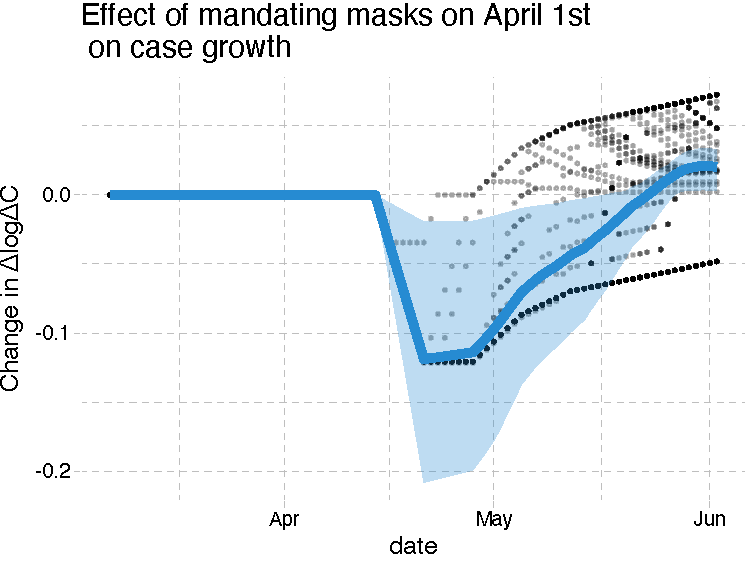
\includegraphics[width=0.49\textwidth]{tables_and_figures/us-mask-dgrowth_v1}
      &
        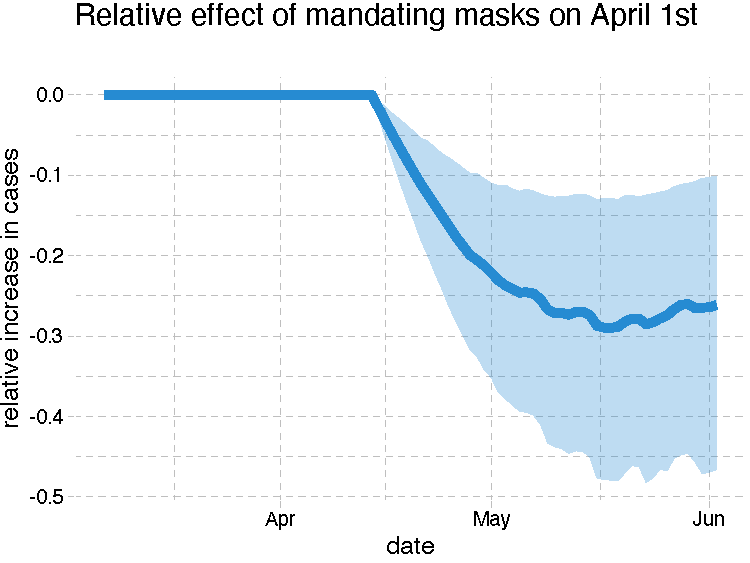
\includegraphics[width=0.49\textwidth]{tables_and_figures/us-mask-rel_v1}
      \\
      \\
      \multicolumn{2}{c}{\textbf{Deaths}} \\
      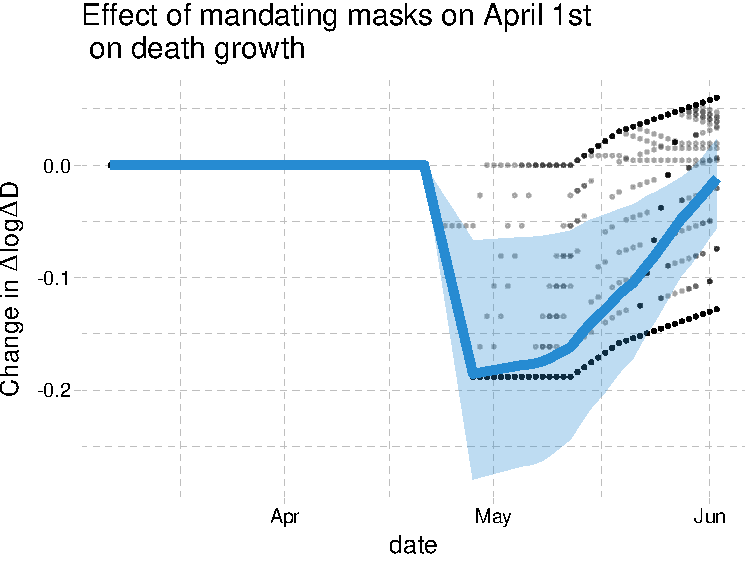
\includegraphics[width=0.49\textwidth]{tables_and_figures/us-mask-dgrowth_deaths_v1}
      &
        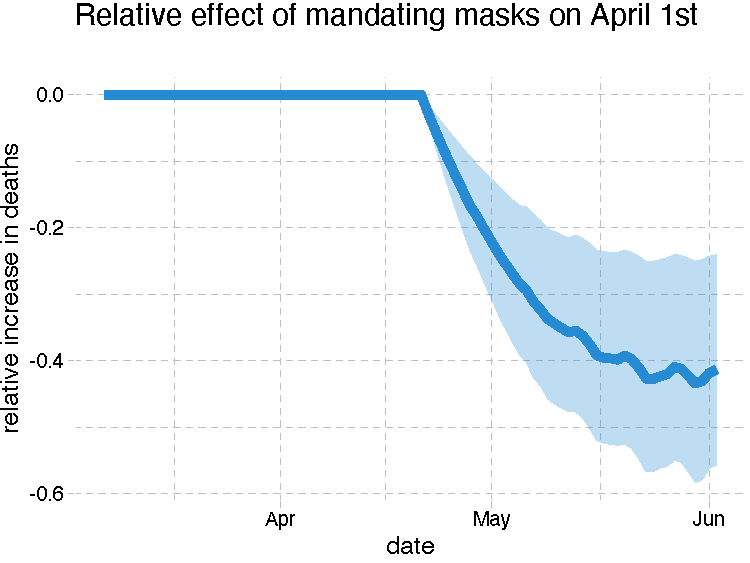
\includegraphics[width=0.49\textwidth]{tables_and_figures/us-mask-rel_deaths_v1}
    \end{tabular}
  \end{minipage}
%    \begin{flushleft}
%      \footnotesize
%      In the left column, the dots are the average change in growth in
%      each state. The blue line is the average across states of the
%      change in growth. The shaded region is a point-wise 90\% confidence
%      interval. The right column shows the change in cases or deaths
%      relative to the baseline of actual policies.
%    \end{flushleft}
\end{figure}

\begin{figure}[ht]
 % \caption{National effect of leaving non-essential businesses open\label{fig:US-nb}}
  \caption{Effect  of   leaving non-essential businesses open on cases in the US  \label{fig:US-nb-dgrowth}}
  \begin{minipage}{\linewidth}
    \centering
    \begin{tabular}{cc}
      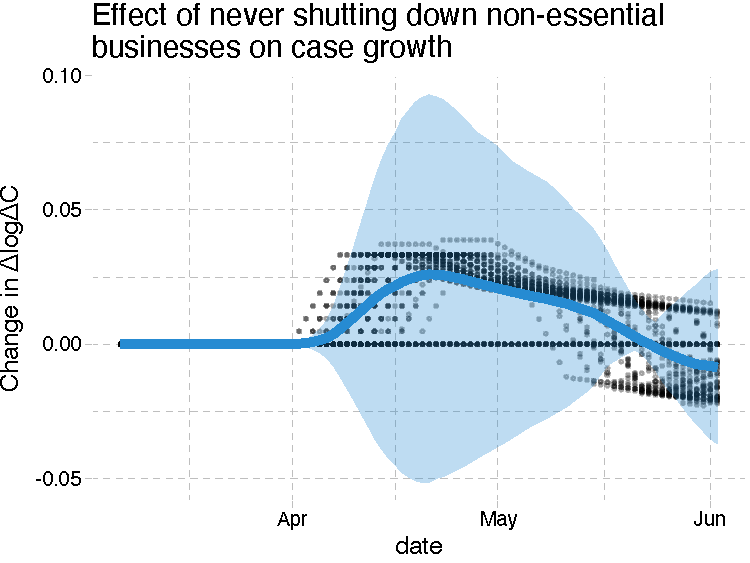
\includegraphics[width=0.45\textwidth]{tables_and_figures/us-nb-dgrowth_v1}
      &
        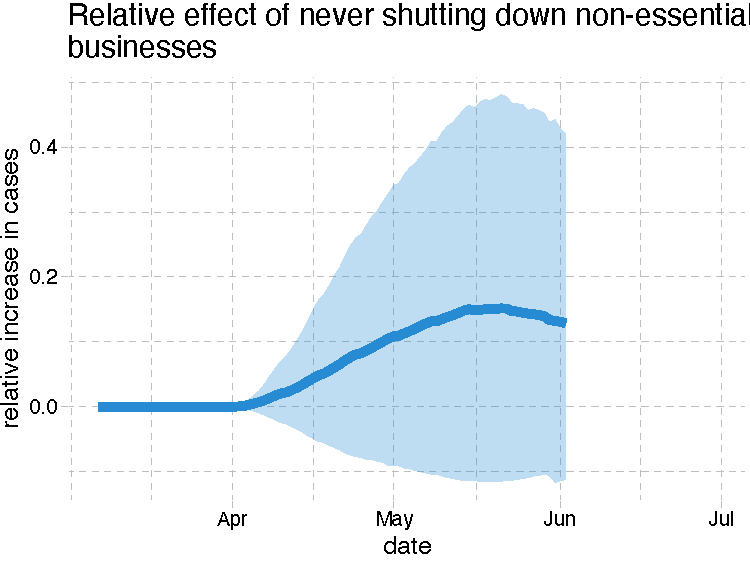
\includegraphics[width=0.45\textwidth]{tables_and_figures/us-nb-rel_v1}
%      \\
%      \includegraphics[width=0.45\textwidth]{tables_and_figures/us-nb-dgrowth_deaths}
%      &
%        \includegraphics[width=0.45\textwidth]{tables_and_figures/us-nb-rel_deaths}
    \end{tabular}
  \end{minipage}
\end{figure}



\begin{figure}[ht]
 % \caption{National effect of leaving non-essential businesses open\label{fig:US-nb}}
  \caption{Effect  of  not implementing stay-at-home order on cases in the US  \label{fig:US-shelter-dgrowth}}
  \begin{minipage}{\linewidth}
    \centering
    \begin{tabular}{cc}
      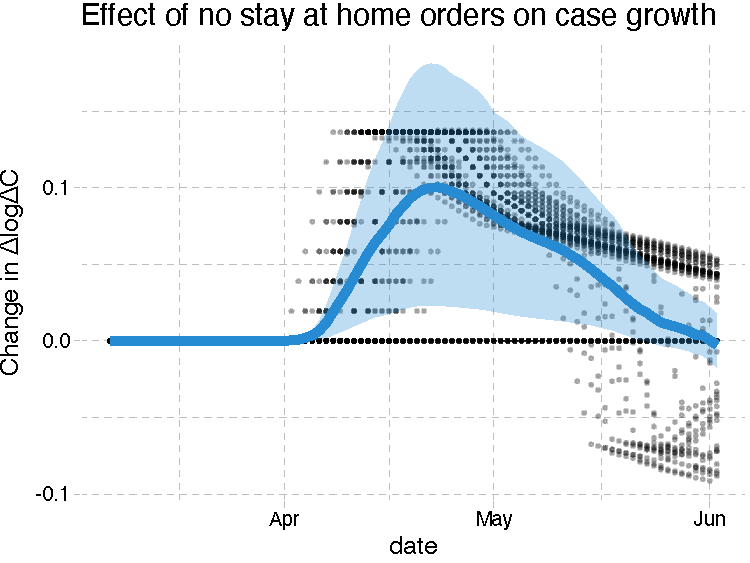
\includegraphics[width=0.45\textwidth]{tables_and_figures/us-shelter-dgrowth_v1}
      &
        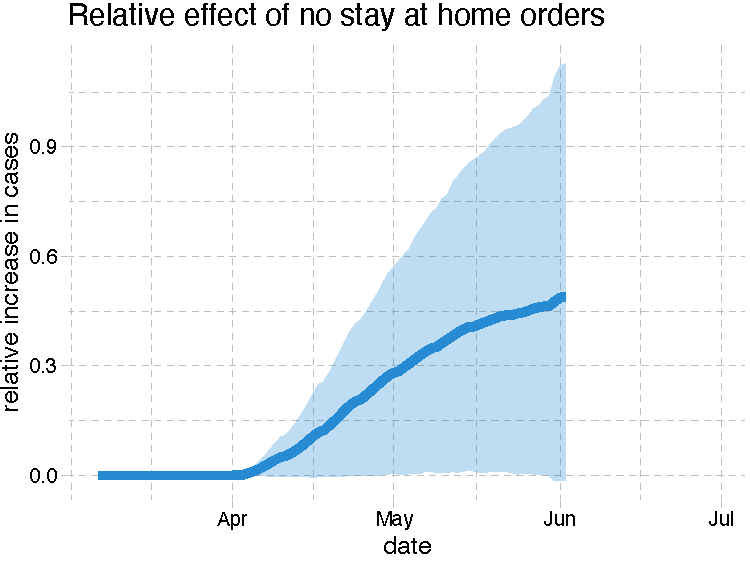
\includegraphics[width=0.45\textwidth]{tables_and_figures/us-shelter-rel_v1}
    \end{tabular}
  \end{minipage}
\end{figure}




%\begin{figure}[ht]
% \caption{Average effect  of removing
%   all policies on cases \label{fig:US-nop-dgrowth}}
%%  \caption{Effect of removing policies: national average \label{fig:US-nop}}
%  \begin{minipage}{\linewidth}
%    \centering
%    \begin{tabular}{cc}
%      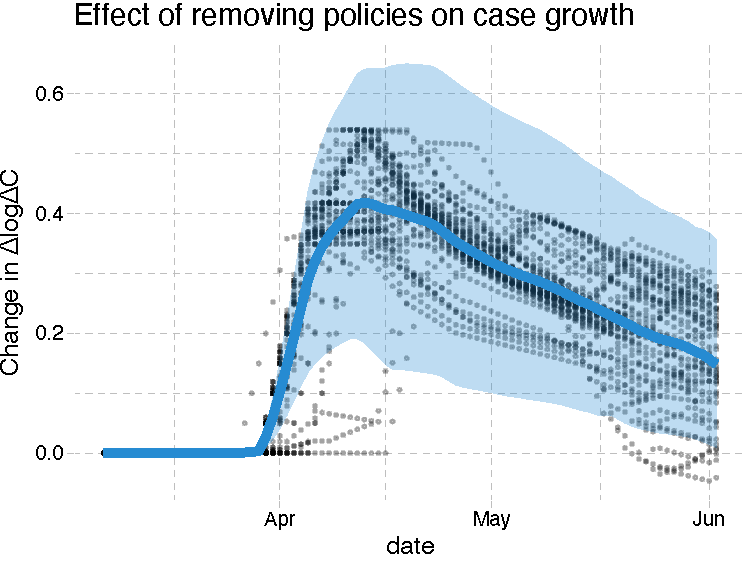
\includegraphics[width=0.45\textwidth]{tables_and_figures/us-nop-dgrowth_v1}
%      &
%        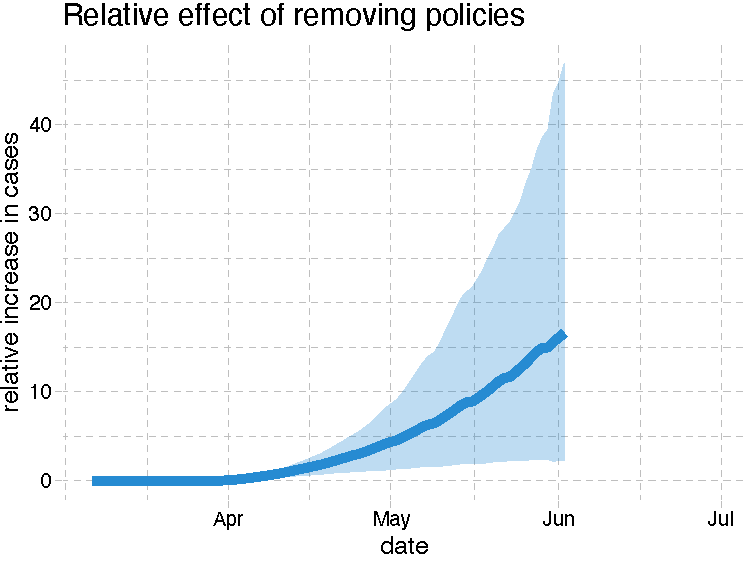
\includegraphics[width=0.45\textwidth]{tables_and_figures/us-nop-rel_v1}
%%      \\
%%      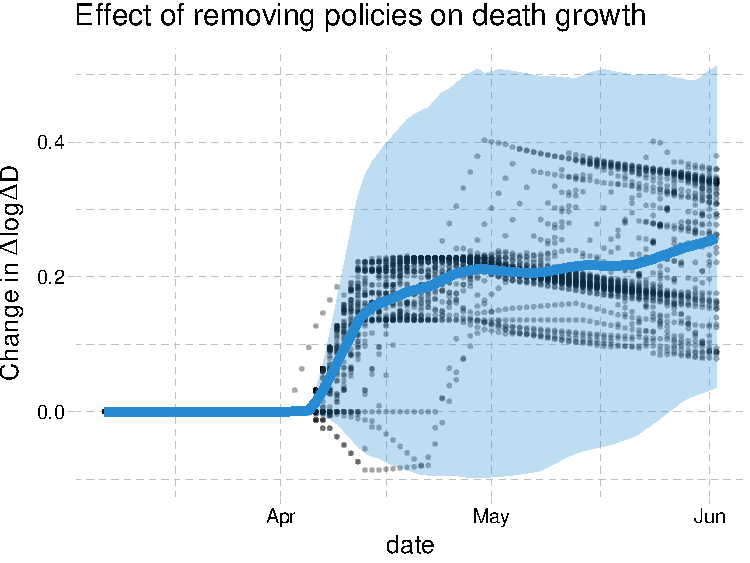
\includegraphics[width=0.45\textwidth]{tables_and_figures/us-nop-dgrowth_deaths}
%%      &
%%        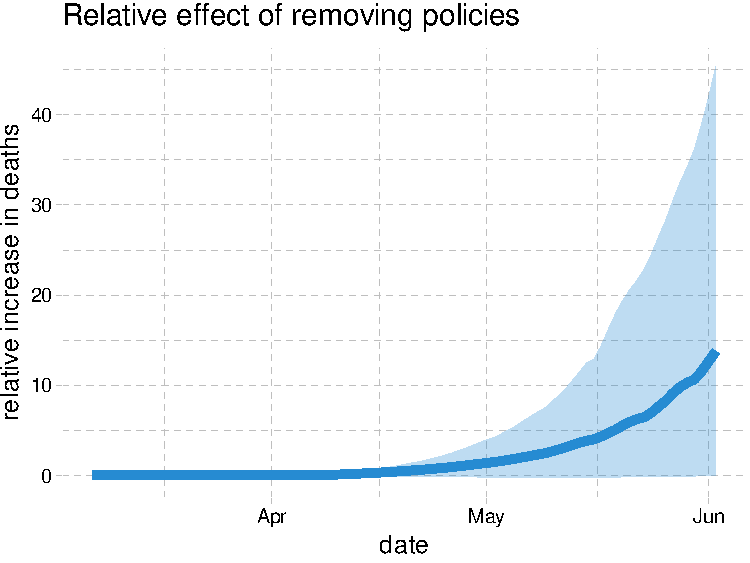
\includegraphics[width=0.45\textwidth]{tables_and_figures/us-nop-rel_deaths}
%    \end{tabular}
%  \end{minipage}
%\end{figure}




%\subsection{Related literature}
%
%
%... and why/how we are different.



A growing number of other papers have examined the link between non-pharmaceutical interventions and Covid-19  cases.\footnote{We refer the reader to \cite{avery2020} for a comprehensive review of  a larger body of work researching Covid-19; here we focus on few quintessential comparisons on our work with other works that we are aware of.} \cite{hsiang2020} estimate the effect of policies on the growth rate of cases using
data from the United States, China, Iran, Italy, France, and South
Korea. In the United States, they find that the combined effect of all policies they consider on the
growth rate is $-0.347$ $(0.061)$. \cite{courtemanche2020} use US county level data to analyze the effect
of interventions on case growth rates. They find that the combination
of policies they study reduced growth rates by 9.1 percentage points
16-20 days after implementation, out of which 5.9 percentage points are attributed to shelter in place orders. Both \cite{hsiang2020} and \cite{courtemanche2020} adopted a reduced-form approach to estimate the total policy effect on case growth without using any social distancing behavior measures. In contrast, our study highlights the role of behavioral response to policies and information.

Existing evidence for the impact of social distancing policies on behavior in the US is mixed.
\cite{abouk2020} employ a difference-in-differences methodology to  find that statewide stay-at-home orders  have  strong causal impacts on reducing social interactions. In contrast, using data from Google Mobility Reports,
\cite{maloney2020}  find that the increase in social distancing is
largely voluntary and driven by information.\footnote{Specifically, they find
that of the 60 percentage point drop in workplace intensity, 40
percentage points can be explained by changes in information as
proxied by case numbers, while roughly 8 percentage points can be
explained by policy changes.} Another study by  \cite{gupta2020} also found little evidence that stay-at-home mandates induced distancing by
using mobility measures from PlaceIQ and SafeGraph. Using data from SafeGraph, \cite{anderson2020} show that there has been substantial voluntary social distancing but also provide evidence that mandatory measures such as stay-at-home orders have  been effective at reducing the frequency of visits  outside of one’s home.
% Overall, these evidence suggests the importance of voluntary social distancing behavior when we evaluate the effect of polices.

 \cite{pei2020} use county-level observations of reported infections and deaths in conjunction with mobility  data from SafeGraph to estimate how effective reproductive numbers in major metropolitan areas change over time. They conduct simulation of implementing all policies 1-2 weeks earlier and found that it would have resulted in reducing the number of cases and deaths by more than half. However, their study does not  explicitly analyze how policies are related to
the effective reproduction numbers. % Our study  analyzes how policies  affects the reproduction numbers through their impact on people's behavior.

Epidemiologists use model simulations to predict how cases and deaths evolve for the purpose of policy recommendation. As reviewed by \cite{avery2020}, there exist substantial uncertainty about the values of key epidimiological parameters \citep[see also][]{atkeson2020b,stock2020}. Simulations are often done under strong assumptions about the impact of social distancing policies without connecting to the relevant data  \citep[e.g.,][]{ferguson2020}. Furthermore, simulated models do not take into account that people may limit their contact with other people in response to higher transmission risks.\footnote{See \cite{atkeson2020a} and \cite{stock2020} for the implications of the SIR model for Covid-19 in the US. \cite{NBERw27128} estimate a SIRD model in which time-varying reproduction numbers depend on the daily deaths to capture feedback from daily deaths
to future behavior and infections.}  When such a voluntary behavioral response is ignored, simulations would produce exponential spread of disease and would over-predict  cases and deaths. Our counterfactual experiments  illustrate the importance of this voluntary behavioral change.




Whether wearing  masks in public place should be mandatory or not has been one of the most contested policy issues with health authorities of different countries providing contradiction recommendations. Reviewing evidence, \cite{Greenhalghm2020}  recognize that there is no randomized controlled trial evidence for the effectiveness of face masks,  but they state ``indirect evidence exists to support the argument for the public wearing masks in the Covid-19 pandemic."\footnote{The virus remains viable in the air for several hours, for which surgical masks may be effective. Also, a substantial fraction of individual who are infected become infectious before showing symptom onset.}
\cite{howard2020} also review available medical evidence and conclude that ``mask wearing reduces the transmissibility per contact by reducing transmission of infected droplets in both laboratory and clinical contexts.''  The laboratory findings in \cite{hou2020} suggest that the nasal cavity may be the initial site of infection followed by aspiration to the lung, supporting the argument  ``for the widespread use of masks to prevent aersol, large droplet, and/or mechanical exposure to the nasal passages.''

Given the lack of experimental evidence on the effect of masks, conducting observational studies  is useful and important. To the best of our knowledge, our paper is the first  empirical study that shows the effectiveness of  mask mandates on reducing the spread of Covid-19 by analyzing the US state-level data. This finding corroborates and is complementary to the medical observational evidence in \cite{howard2020}. Analyzing mitigation measures in New York, Wuhan, and Italy, \cite{zhangr2020} conclude that mandatory face coverings substantially reduced infections. \cite{abaluck2020}  find that the growth rates of cases and of deaths in countries with pre-existing norms that sick people should wear masks are lower by 8 to 10\% than those rates in countries with no pre-existing mask norms. Our finding
is also corroborated by a completely different causal methodology based on synthetic control 
using German data in \cite{Mitze2020}.\footnote{Our study was first released in ArXiv on May 28, 2020 whereas
 \cite{Mitze2020} was released at SSRN on June 8, 2020.}

Our empirical results contribute to informing the economic-epidemiological models that combine economic models with variants of SIR models to evaluate the efficiency of various economic policies aimed at gradual ``reopening" of various sectors of economy.\footnote{\cite{adda2016} analyzes the effect of policies reducing interpersonal contacts such as school closures or the closure of public transportation networks on the spread of  influenza, gastroenteritis, and chickenpox using high frequency data from France.} For example, the estimated effects of masks, stay-home mandates, and various other policies on behavior, and of behavior on infection can serve as useful inputs and validation checks in the calibrated macro, sectoral, and micro models (see, e.g., \cite{alvarez2020simple,baqaee2020reopening,NBERw27128,acemoglu2020multi,lsmith,nashSIR} and references therein). Furthermore, the causal framework developed in this paper could be applicable, with appropriate extensions, to the impact of policies on economic outcomes replacing health outcomes (see, e.g., \cite{chetty2020real,coibion2020labor}).



\section{The Causal Model for the Effect of Policies, Behavior, and Information on Growth of Infection}\label{sec:causal-model}

\subsection{The Causal Model and Its Structural Equation Form}
We introduce our approach through the Wright-style causal diagram shown in Figure \ref{Wright}.  The diagram describes how policies, behavior, and information interact together:
\begin{itemize}
\item The \textit{forward} health outcome,
$Y_{i,t+\ell}$, is determined last, after all other variables have been determined;
\item The  adopted policies, $P_{it}$,  affect health outcome $Y_{i,t+\ell}$ either directly, or indirectly by altering  human behavior  $B_{it}$;
\item  Information variables, $I_{it}$, such as lagged values of outcomes can affect human behavior and  policies, as well as  outcomes;
\item The confounding factors $W_{it}$, which vary across states and time, affect all other variables.
\end{itemize}
The index $i$ denotes observational unit, the state, and $t$ and $t+\ell$ denotes the time, where  $\ell$ represents the time lag  between infection and case confirmation or death.
\begin{figure}[ht]
\begin{center}
\begin {tikzpicture}[-latex, auto, node distance =1.5cm and 3cm, on grid, thick,
  empty/.style ={circle, top color=white, bottom color = white, draw, white, text=white , minimum width =1.25 cm},
  policy/.style ={circle, top color=white, bottom color = blue, draw, black, text=black , minimum width =1.25 cm},
    behavior/.style ={circle, top color=white, bottom color = ForestGreen, draw, black, text=black , minimum width =1.25 cm},
  observed/.style ={circle, top color=white, bottom color = magenta, draw, black, text=black , minimum width =1.25 cm} ,
   confounder/.style ={circle, top color=white, bottom color =  gray, draw, black, text=black , minimum width =1.25 cm} ,
outcome/.style ={circle, top color=white, bottom color = red, draw, black, text=black , minimum width =1.25 cm} ]

\node[policy]   (P) {\tiny $P_{it}$};
\node[empty] (E) [below=of P] {\tiny $I_{it}$};
\node[outcome]  (Y)[ right =of E] {\tiny $Y_{i,t+\ell}$};
\node[behavior] (B) [below =of E] {\tiny $B_{it}$};
\node[observed] (I) [left =of P] {\tiny $I_{it}$};
\node[confounder] (W) [left=of B] {\tiny  $W_{it}$};
\path[->] (P) edge (Y);
\path[->] (B) edge (Y);
\path[->] (P) edge (B);
\path[->] (I) edge (B);
\path[->] (I) edge (P);
\path[->] (W) edge (Y);
\path[->] (W) edge (B);
\path[->] (W) edge (P);
\path[->] (W) edge (I);
\path[->] (I) edge (Y);

\end{tikzpicture} \end{center}
\caption{S. \& P. Wright type causal path diagram for our model. }\label{Wright}
\end{figure}

Our main outcomes of interest are the growth rates in Covid-19 cases and deaths,  behavioral variables include proportion of time spent in transit or shopping and others, policy variables include stay-at-home orders and school and business closures, and the information variables include lagged values of outcome. We provide a detailed description of these variables and their timing in the next section.


The causal structure  allows for  the effect of the policy to be either direct or indirect -- through-behavior or through dynamics; and all of these effects are not mutually exclusive. The structure also allows for changes in behavior to be brought by change in policies and information. These are all realistic properties that we expect from the contextual knowledge of the problem. Policies such as closures of schools, non-essential business, and restaurants, alter and constrain behavior in strong ways.  In contrast, policies such as mandating employees to wear masks can potentially affect the Covid-19 transmission directly.  The information variables, such as recent growth in the number of cases, can cause people to spend more time at home, regardless of adopted state policies; these changes in
behavior in turn affect the transmission of Covid-19.

The causal ordering induced by this directed acyclical graph is determined by the following
timing sequence: % \textit{within a period}:%\footnote{Mathematically this corresponds to the factorization of the data likelihood, omitting indexes, $$f_{Y,P,B, I, W} = f_{Y\mid P, B,I, W} f_{B \mid P,I,W } f_{P \mid I, W} f_{I,W}.$$ }
\begin{itemize}
\item[(1)]  information and confounders get determined at $t$,
\item[(2)] policies are set in place, given information and confounders at $t$;
\item[(3)] behavior is realized, given policies, information, and confounders at $t$;
\item[(4)] outcomes get realized at $t+\ell$ given policies, behavior, information, and confounders.
\end{itemize}

The model also allows for direct dynamic effects of information variables on the outcome through autoregressive structures that capture persistence in growth patterns. As  highlighted below, realized outcomes may become new information for future periods, inducing dynamics over multiple periods.



Our quantitative model for causal structure in Figure \ref{Wright} is given by the following econometric structural equation model:\begin{equation} \label{eqn:SEM1} \tag{SEM}
  \begin{aligned}
   &  Y_{i,t+\ell} (b,p,\iota) &:=& {\bcolor \alpha ' b}  +  {\pcolor \pi 'p} +
    {\icolor \mu'\iota } + {\wcolor \delta_Y 'W_{it}} + \varepsilon^y_{it}, \\
   &  B_{it} (p,\iota) &:= & {\pcolor \beta'p } + {\icolor \gamma'\iota} +      {\wcolor\delta_B 'W_{it} } + \varepsilon^b_{it},
      \end{aligned}
 \end{equation}
which is a collection of functional relations with stochastic shocks, decomposed into observable part $\delta' W$ and unobservable part $\varepsilon$.
The terms $\varepsilon^y_{it}$ and  $\varepsilon^b_{it} $  are the centered stochastic shocks that obey the orthogonality restrictions posed below.


The policies can be modeled via a linear form as well,
\begin{equation}\label{eq:Policy} \tag{P}
 P_{it}   (\iota) :=  {\icolor\eta'\iota} + {\wcolor \delta_P' W_{it}} +   \varepsilon^p_{it},   \end{equation}
although  linearity is not critical.\footnote{Under some additional independence conditions, this
can be replaced by an arbitrary non-additive function $P_{it}(\iota) = p (\iota, W_{it},  \varepsilon^p_{it})$, such that the unconfoundedness condition stated in the next footnote holds.}


The orthogonality restrictions on the stochastic components are as follows:
\begin{equation}\label{eqn:SEM2} \tag{O}
\begin{aligned}
   & \varepsilon^y_{it} &  \perp &  \quad (\varepsilon^b_{it}, \varepsilon^p_{it}, {\wcolor W_{it}}, {\icolor I_{it}}), \\
&  \varepsilon^b_{it}  & \perp & \quad  (\varepsilon^p_{it}, {\wcolor W_{it}}, {\icolor I_{it}}), \\
&   \varepsilon^p_{it} &  \perp &  \quad ({\wcolor W_{it}}, {\icolor I_{it}}),
\end{aligned}
\end{equation}
where we say that $V \perp U$ if $\Ep VU = 0$. This is a standard way of representing restrictions on errors in structural equation modeling.\footnote{ An alternative useful
starting point is to impose the Rubin-Rosenbaum type unconfoudedness condition:
$$
Y_{i,t+\ell} (\cdot,\cdot,\cdot)  \indep (P_{it}, B_{it}, I_{it})  \mid W_{it}, \
B_{it} (\cdot,\cdot)  \indep (P_{it}, I_{it})  \mid W_{it}, \
 P_{it} (\cdot)  \indep  I_{it}  \mid W_{it},
$$
which imply, with treating stochastic errors as independent additive components, the orthogonal conditions stated above.
 }\footnote{The structural equations of this form are connected to triangular structural equation models, appearing
 in microeconometrics and macroeconometrics (SVARs), going back to the work of  \cite{strotz1960recursive}. .}


 The observed variables are generated by setting $\iota = I_{it}$ and propagating
the system from the last equation to the first:
%\begin{equation} \label{eqn:SEM2}
\[
  \begin{aligned}
& {\ycolor Y_{i,t+\ell}}  & := & Y_{i,t+\ell} ( {\bcolor B_{it} } ,{\pcolor P_{it}}, {\icolor I_{it}}), \\
& {\bcolor B_{it} } & := &   B_{it}({\pcolor P_{it} } ,{\icolor I_{it}}), \\
& {\pcolor P_{it} }& := &  P_{it}({\icolor I_{it}}). \end{aligned}
\]
%\end{equation}


The system above together with  orthogonality restrictions (\ref{eqn:SEM2}) implies the following collection of stochastic equations for realized variables:
\begin{align}
   &  {\ycolor  Y_{i,t+\ell}}
    = {\bcolor\alpha ' B_{it}} + {\pcolor\pi 'P_{it}} + {\icolor\mu'I_{it}} + {\wcolor\delta_Y 'W_{it}}  + \varepsilon^y_{it},
    &  & \varepsilon^y_{it} \perp {\bcolor B_{it}}, {\pcolor P_{it}}, {\icolor I_{it}}, {\wcolor W_{it}} \label{eq:R1} \tag{BPI$\to$Y} \\
    &  {\bcolor B_{it}}
     =  {\pcolor \beta' P_{it}} + {\icolor \gamma'I_{it}} +  {\wcolor \delta_B' W_{it}} + \varepsilon^b_{it},
   & & \varepsilon^b_{it} \perp {\pcolor P_{it}}, {\icolor I_{it}}, {\wcolor W_{it}}  \label{eq:R2} \tag{PI$\to$B}  \\
    & {\pcolor P_{it}}
    =  {\icolor\eta'I_{it}} + {\wcolor \delta_P' W_{it}} +   \varepsilon^p_{it},   & & \varepsilon^p_{it} \perp   {\icolor I_{it}}, {\wcolor W_{it}} \label{eq:R3}  \tag{I$\to$P}
       \end{align}
and
\begin{equation}
   {\ycolor  Y_{i,t+\ell}}
   = ( {\bcolor\alpha '}  {\pcolor \beta' }+{\pcolor\pi'} )
    {\pcolor P_{it}} + ( {\bcolor\alpha '}  {\icolor \gamma'} + {\icolor \mu'})
    {\icolor I_{it} }+ {\wcolor \bar{\delta} '}{\wcolor W_{it}}  + {\bar \varepsilon}_{it},  \quad   {\bar \varepsilon}_{it} \perp
  {\pcolor P_{it}},  {\icolor I_{it}}, {\wcolor W_{it}}.  \label{eq:R4} \tag{PI$\to$Y}
\end{equation}
These equations form the basis of our empirical analysis.

As discussed below, the information variable includes case growth. Therefore,  an orthogonality restriction  $ \varepsilon^y_{it} \perp   {\pcolor P_{it}}$ holds if  the government does not have knowledge on future case growth beyond what is predicted by today's case growth, policies,  behavior, and  confounders; even when the government has some knowledge on $\varepsilon^y_{it}$, the orthogonality restriction may hold if there is a time lag for the government to implement its policies based on $\varepsilon^y_{it}$.

The orthogonality condition in (\ref{eq:R4}) is weaker than the orthogonality conditions in  (\ref{eq:R1})-(\ref{eq:R2}) in that the former is implied by the latter but not vice versa.
The system over-identifies the regression coefficients because  $({\bcolor\alpha '}  {\pcolor \beta' }+{\pcolor\pi'})$ and $({\bcolor\alpha '}  {\icolor \gamma'} + {\icolor \mu'})$ in  (\ref{eq:R4}) can be also identified from  ${\bcolor\alpha ' }$,  $ {\pcolor\pi '}$, ${\icolor\mu'}$,   ${\pcolor \beta' }$, and ${\icolor \gamma'}$ in (\ref{eq:R1})-(\ref{eq:R2}).  Comparing the estimates of $({\bcolor\alpha '}  {\pcolor \beta' }+{\pcolor\pi'})$ and $({\bcolor\alpha '}  {\icolor \gamma'} + {\icolor \mu'})$ from  (\ref{eq:R4})  with  those implied by  the estimates of ${\bcolor\alpha ' }$,  $ {\pcolor\pi '}$, ${\icolor\mu'}$,   ${\pcolor \beta' }$, and ${\icolor \gamma'}$ from   (\ref{eq:R1})-(\ref{eq:R2}) provides a useful specification test.


\subsection*{Identification and Parameter Estimation}

The orthogonality equations imply that these are all projection equations, and the parameters of the SEM are identified by the parameters of these regression equation, provided the latter are identified by sufficient joint variation of these variables across states and time.


The last point can be stated formally as follows. Consider the previous system of equations, after partialling out the confounders:
\begin{equation}\label{eqn:SEM-PO}
 \begin{aligned}
   & {\ycolor { \tilde Y_{i,t+\ell}}}  & =& {\bcolor {\alpha ' \tilde B_{it}}} +{\pcolor {\pi '\tilde P_{it}}} +{\icolor \mu'\tilde I_{it} } + \varepsilon^y_{it},&\varepsilon^y_{it} &\perp {\tilde B_{it}}, {\tilde  P_{it}}, { \tilde I_{it}},  \\
   & {\bcolor { \tilde B_{it}}} & = &{\pcolor { \beta' \tilde P_{it}} } + {\icolor { \gamma' \tilde I_{it}} } + \varepsilon^b_{it},
   &\quad \varepsilon^b_{it} &\perp { \tilde P_{it}}, { \tilde I_{it}},  \\
   & {\pcolor { \tilde P_{it}} } &= &  {\icolor {\eta' \tilde I_{it}} } +   \varepsilon^p_{it}, &\quad \varepsilon^p_{it} &\perp {\tilde I_{it}}  \\
  \end{aligned}
\end{equation}
where $ \tilde V_{it} = V_{it}   -     {\wcolor W_{it}'} \Ep[{\wcolor W_{it}W_{it}'}]^{-} \Ep[{\wcolor W_{it}} V_{it}]$ denotes
the residual after removing the orthogonal projection of $V_{it}$ on ${\wcolor W_{it}}$. The residualization is a linear operator, implying that (\ref{eqn:SEM-PO}) follows immediately from the above. The parameters of (\ref{eqn:SEM-PO})  are identified as projection coefficients in these equations, provided that residualized vectors appearing in each of the equations have non-singular variance, that is
 \begin{equation}
 \Var ( {\pcolor \tilde P_{it}'} ,{\bcolor \tilde B_{it}'},{\icolor \tilde I_{it}'})>0,
 \ \Var ({\pcolor \tilde P_{it}'}, {\icolor \tilde I_{it}'})> 0 , \ \text{ and  }  \Var ( {\icolor \tilde I_{it}'}) >0.
 \end{equation}

Our main estimation method is the standard correlated random effects estimator, where the random effects
are parameterized as functions of observable characteristic, ${\wcolor W_{it}}$, which include both state-level and time random effects.  The state-level random effects
are modeled as a function of state level characteristics, and the time random effects are modeled
by including month dummies and their interactions with state level characteristics.  The stochastic shocks $\{ \varepsilon_{it}\}_{t=1}^T$
are treated as independent across states $i$ and can be arbitrarily dependent across time $t$ within a state.

A secondary estimation method is the fixed effects estimator, where ${\wcolor W_{it}}$ includes
latent (unobserved) state level effects ${\wcolor W_i}$ and  and time level effects ${\wcolor W_t}$,
which must be estimated from the data.  This approach is much more demanding of the data and relies on long cross-sectional
and time histories. When histories are relatively short,  large biases emerge and
they need to be removed using debiasing methods. In our context, debiasing
  changes the estimates substantially, often changing the sign of coefficients.\footnote{This is a pre-cautionary
message that may be useful for other researchers using fixed effects estimators in the context
of Covid-19 analysis. We recommend using debiased fixed effects estimators, see e.g., \cite{chen2019mastering}
for expository treatment. }
However, we find the debiased fixed effect estimates are
qualitatively and quantitatively similar to the correlated random effects estimates.
Given this finding, we chose to focus on the latter, as it is a more standard and familiar method, and report the former
estimates in the supplementary materials for this paper.\footnote{The similarity of the debiased fixed
effects and correlated random effects served as a useful specification check. Moreover, using the fixed
effects estimators only yielded minor gains in predictive performances, as judging by the adjusted
$R^2$'s, providing another useful specification check.}

\subsection{Information Structures and Induced Dynamics}  We consider three examples of information
structures: Information variable is  a function of time:
$${\icolor I_{it}} = g(t);$$
 Information variable is lagged value of outcome:
$$
{\icolor I_{it}} =  {\ycolor Y_{it}};
 $$
 and finally:
 \begin{itemize}
 \item[(\textsc{I})] Information variables include time, lagged and integrated values of outcome:
 $$
{\icolor I_{it}} = \left (g(t) , {\ycolor Y_{it}},  \sum_{m=0}^{t/\ell}
{\ycolor Y_{i,t - \ell m}} \right) ',
 $$
 with the convention that ${\ycolor Y_{it}} = 0$  for $t \leq 0$.
\end{itemize}
The first information structure captures the  basic idea that, as individuals discover more information about covid over time, they adapt to safer modes of  behavior (stay-at-home, wear masks, wash hands). {Under this structure, information is common across states and exogenously evolves over time, independent of the number of cases.}
The second  structure  arises from considering
autoregressive components {and captures people's behavioral response to information on cases in the state they reside}.  {Specifically,} we model persistence in growth rates, ${\ycolor Y_{i,t+\ell}}$, through an AR(1) model, which leads to ${\icolor I_{it}}= {\ycolor Y_{it}}$. This provides useful \textit{local}, state-specific, information about the forward growth rate and people may adjust their behavior to safer modes when they see a high value. We model this adjustment via the term ${\icolor \gamma'I_{t}}$ in the behavior equation. The {third information} structure
is the combination of the first two structures plus an additional  term representing the log of the total number of new cases in the state. We use this information structure in our empirical specification. In this structure, people respond to both global information, captured by a function of time such as month dummies, and local information sources, captured by the local growth rate and the total number of cases.
The last element of the information set can be thought of as a local stochastic trend in cases.

All of these examples fold into a specification of the form:
\begin{equation}\label{eq:I}\tag{I}
 {\icolor I_{it} } :=   I_{it}({\icolor I_{i,t-\ell}}, {\ycolor Y_{it}}, t),  \quad t =1,..., T,
 \end{equation}
 with the initialization ${\icolor I_{i 0}} = 0$ and ${\ycolor Y_{i0}} = 0$.\footnote{This initialization is appropriate
 in our context for analyzing pandemics from the very beginning, but other initializations could be appropriate in other contexts. The  lagged values of behavior variable may be also included in the information set.
 }

With any structure of this form, realized outcomes may become new information for future periods, inducing a dynamical system over multiple periods. We show the resulting dynamical system in a causal diagram of Figure \ref{fig:DynS}.  Specification
of this system is useful for studying delayed effects of policies and behaviors and in considering the counterfactual policy analysis.

\begin{figure}[ht]
\begin{center}
\begin {tikzpicture}[-latex, auto, node distance =3cm and 3cm, on grid, thick,
  empty/.style ={circle, top color=white, bottom color = white, draw, white, text=white , minimum width =1.25 cm},
  policy/.style ={circle, top color=white, bottom color = blue, draw, black, text=black , minimum width =1.25 cm},
    behavior/.style ={circle, top color=white, bottom color = ForestGreen, draw, black, text=black , minimum width =1.25 cm},
  observed/.style ={circle, top color=white, bottom color = magenta, draw, black, text=black , minimum width =1.25 cm} ,
   confounder/.style ={circle, top color=white, bottom color =  gray, draw, black, text=black , minimum width =1.25 cm} ,
outcome/.style ={circle, top color=white, bottom color = red, draw, black, text=black , minimum width =1.25 cm},
myarrow/.style={-Stealth}]

\node[observed] (I)  {\tiny $I_{i,t-\ell}$};
\node[outcome]  (Y)[below=of I ]{\tiny $Y_{it}$};
\node[observed] (In)  [right=of I ]{\tiny $I_{it}$};
\node[outcome]  (Yn)[below=of In ]{\tiny $Y_{i,t+\ell}$};
\node[observed] (Inn)  [right=of In ]{\tiny $I_{i,t+\ell}$};
\node[outcome]  (Ynn)[below=of Inn ]{\tiny $Y_{i,t+2\ell}$};
 \draw [->] (I) -- node[sloped,font=\small,below] {\tiny SEM(t-$\ell$)} (Y);
 \draw [->] (I) --  (In);
 \draw [->] (In) -- node[sloped,font=\small,below] {\tiny SEM(t)} (Yn);
\draw [->] (Y) --  (In);
\draw [->] (In) --  (Inn);
 \draw [->] (Inn) -- node[sloped,font=\small,below] {\tiny SEM(t+$\ell$) } (Ynn);
\draw [->] (Yn) --  (Inn);


\end{tikzpicture} \end{center}
\caption{ Dynamic System Induced by Information Structure and SEM}\label{fig:DynS}
\end{figure}



%
%\subsection{Outcome and Key Confounders via SIR model}\label{sec:sirmodel}
%Letting $C_{it}$ denotes cumulative number of  confirmed cases in state $i$ at time $t$, our outcome
%\begin{equation} \label{eq:y}
%{\ycolor Y_{it}} :=\Delta \log(\Delta C_{it}):= \log( \Delta C_{it} ) -
%\log( \Delta C_{i,t-7})
%\end{equation}
%approximates the weekly growth rate in new cases from $t-7$ to $t$.\footnote{We may show that $ \log( \Delta C_{it} ) -
%\log( \Delta C_{i,t-7})$ approximates the average
%growth rate of cases from $t-7$ to $t$.} Here $\Delta$ denotes the differencing operator over 7 days from $t$ to $t-7$, so that $\Delta C_{it}:=C_{it}-C_{i,t-7}$ is the number of new confirmed cases in the past 7 days.
%
%
%We chose this metric as this is the key metric for policy makers deciding when to relax Covid mitigation policies.  The U.S. government's guidelines for state reopening
%recommend that states display a
%``downward trajectory of documented cases within a 14-day period''
%\citep{whitehouse2020}. A negative value of
%$Y_{it}$ is an indication of meeting this
%criteria for reopening. By focusing on weekly cases  rather than daily cases, we smooth idiosyncratic daily fluctuations as well as periodic fluctuations associated with days of the week.
%
%Our measurement equation for estimating equations (\ref{eq:R1}) and (\ref{eq:R4}) will take the form:
%\begin{align}
%{\ycolor Y_{it}}  =      \theta' X_{it}  + \delta_T \Delta   \log(T)_{it}  +
% \delta_D \frac{T_{it}\Delta D_{it}}{\Delta C_{it}}  + \epsilon_{it},
% \label{eq:M} \tag{M}
%\end{align}
%where $i$ is state, $t$ is day, $C_{it}$ is cumulative confirmed
%cases, $D_{it}$ is deaths, $T_{it}$ is the number of tests over 7 days, $\Delta$ is
%a 7-days differencing operator, $\epsilon_{it}$ is an unobserved error term,
%where $X_{it}$ collects other behavioral, policy, and confounding variables, depending
%on whether we estimate (\ref{eq:R1}) or (\ref{eq:R4}).  Here $$\Delta   \log(T)_{it} \ \text {and } \ \delta_D \frac{T_{it}\Delta D_{it}}{\Delta C_{it}}$$ are the key confounding variables,
%derived from considering the SIR model below. We describe other confounders in the empirical section.
%
% Our main estimating equation (M) is motivated by a variant of a SIR
%model, where we incorporate a
%delay between infection and death instead of a constant death rate,
%and we add confirmed cases to the model. Let $S$, $I$, $\mathcal{R}$, and $D$ denote the number of susceptible,
%infected, recovered, and dead individuals in a given state or
%province. Each of these variables are a function of time. We model
%them as evolving as
%\begin{align}
%  \dot{S}(t) & = -\frac{S(t)}{N} \beta(t) I(t) \label{eq:s} \\
%  \dot{I}(t) & = \frac{S(t)}{N} \beta(t) I(t) - \frac{S(t-\ell)}{N}
%               \beta(t-\ell) I(t-\ell) \label{eq:i} \\
%  \dot{\mathcal{R}}(t) & = (1-\pi) \frac{S(t-\ell)}{N} \beta(t-\ell)
%                         I(t-\ell) \label{eq:r} \\
%  \dot{D}(t) & = \pi \frac{S(t-\ell)}{N} \beta(t-\ell) I(t-\ell) \label{eq:d}
%\end{align}
%where $N$ is the population, $\beta(t)$ is the rate of infection
%spread, $\ell$ is the duration between infection and
%death, and $\pi$ is the
%probability of death conditional on infection.\footnote{The model can easily be extended to allow a
%  non-deterministic disease duration. This leaves our main estimating
%  equation (\ref{eq:c2}) unchanged, as long as the distribution of
%  duration between infection and death is equal to the distribution of
%  duration between infection and recovery.}
%
%Confirmed cases, $C(t)$, evolve as
%\begin{equation}
%  \dot{C}(t) = \tau(t) I(t), \label{eq:c}
%\end{equation}
%where $\tau(t)$ is the rate that infections are detected.
%
%Our goal is to examine how the rate of infection $\beta(t)$ varies with observed policies
%and measures of social distancing behavior. A key challenge is that we only
%observed $C(t)$ and $D(t)$, but not $I(t)$. The unobserved $I(t)$ can
%be eliminated by differentiating (\ref{eq:c}) and using (\ref{eq:i}) and (\ref{eq:d}) as
%\begin{align}
%%  \ddot{C}(t) & = \dot{\tau}(t) + \dot{I}(t) \notag \\
%%  & = \dot{\tau}(t)I(t) + \frac{S(t)}{N} \beta(t) I(t) -
%%    \frac{S(t-\ell)}{N} \beta(t-\ell) I(t-\ell)  \notag \\
%%  & = \dot{\tau}(t) I(t) + \frac{S(t)}{N} \beta(t) I(t) -
%%    \frac{1}{\pi} \dot{D}(t) \notag \\
%  \frac{\ddot{C}(t)}{\dot{C}(t)}
%              & =
%                \frac{S(t)}{N} \beta(t)  + \frac{\dot{\tau}(t)}{\tau(t)}  -
%                \frac{1}{\pi}
%                \frac{\tau(t)\dot{D}(t)}{\dot{C}(t)}. \label{eq:c2}
%\end{align}
%We consider a discrete-time analogue of equation (\ref{eq:c2}) to motivate our empirical
%specification by relating the detection rate $\tau(t)$  to the number of tests $T_{it}$ while specifying $\frac{S(t)}{N}\beta(t)$ as a linear function of variables $X_{it}$.
%This results in
%\begin{align}
%  \underbracket{Y_{it}}_{\frac{\ddot{C}(t)}{\dot{C}(t)}}
%  =
%      \underbracket{X_{it}' \theta + \epsilon_{it}}_{\frac{S(t)}{N}\beta(t)} +
%       & \underbracket{\delta_T \Delta
%      \log(T)_{it}}_{\frac{\dot{\tau}(t)}{\tau(t)} } +
%      \underbracket{\delta_D \frac{T_{it}\Delta D_{it}}{\Delta C_{it}}  }_{\frac{1}{\pi}
%      \frac{\tau(t)\dot{D}(t)}{\dot{C}(t)}}, \nonumber % \label{eq:reg2}
%\end{align}
%which is equation (\ref{eq:M}), where $X_{it}$ captures a vector of variables related to $\beta(t)$.
%
%\begin{quote}
%\textsc{Structural Interpretation}. In the early pandemics, when
%the number of susceptibles is approximately the same as the entire population, i.e. $S_{it}/N_{it} \approx 1$, the component $X_{it}' \theta$
%is the projection of infection rate $ \beta_i(t)$ on   $X_{it}$ (policy, behavioral, information, and confounders other than testing rate), provided
%the stochastic component $\epsilon_{it}$ is orthogonal
%to $X_{it}$ and the testing variables:
%$$
%\beta_i(t)S_{it}/N_{it}  = X_{it}' \theta + \epsilon_{it}, \quad \epsilon_{it} \perp X_{it}.
%$$
%\end{quote}

\subsection{Outcome and Key Confounders via SIR model}\label{sec:sirmodel}
Letting $C_{it}$ denote the cumulative number of  confirmed cases in state $i$ at time $t$, our outcome
\begin{equation} \label{eq:y}
{\ycolor Y_{it}} =\Delta \log(\Delta C_{it}):= \log( \Delta C_{it} ) -
\log( \Delta C_{i,t-7})
\end{equation}
approximates the weekly growth rate in new cases from $t-7$ to $t$.\footnote{We may show that $ \log( \Delta C_{it} ) -
\log( \Delta C_{i,t-7})$ approximates the average
growth rate of cases from $t-7$ to $t$.} Here $\Delta$ denotes the differencing operator over 7 days from $t$ to $t-7$, so that $\Delta C_{it}:=C_{it}-C_{i,t-7}$ is the number of new confirmed cases in the past 7 days.


We chose this metric as this is the key metric for policy makers deciding when to relax Covid mitigation policies.  The U.S. government's guidelines for state reopening
recommend that states display a
``downward trajectory of documented cases within a 14-day period''
\citep{whitehouse2020}. A negative value of
$Y_{it}$ is an indication of meeting this
criteria for reopening. By focusing on weekly cases  rather than daily cases, we smooth idiosyncratic daily fluctuations as well as periodic fluctuations associated with days of the week.

Our measurement equation for estimating equations (\ref{eq:R1}) and (\ref{eq:R4}) will take the form:
\begin{align}
{\ycolor \Delta \log(\Delta C_{it})}  =    X_{i,t-14} '   \theta  -\gamma +  \delta_T \Delta   \log(T_{it})  + \epsilon_{it},
% \delta_D \frac{T_{it}\Delta D_{it}}{\Delta C_{it}}  + \epsilon_{it},
 \label{eq:M} \tag{M-C}
\end{align}
where $i$ is state, $t$ is day, $C_{it}$ is cumulative confirmed
cases, $T_{it}$ is the number of tests over 7 days, $\Delta$ is
a 7-days differencing operator, $\epsilon_{it}$ is an unobserved error term.
 $X_{i,t-14}$  collects other behavioral, policy, and confounding variables, depending
on whether we estimate (\ref{eq:R1}) or (\ref{eq:R4}), where the lag of $14$ days captures the time lag between infection and confirmed case (see the Appendix \ref{sec:timing}). %for available evidence on a delay between infection and confirmation of cases or deaths.
   Here
$$\Delta   \log(T_{it} ):=  \log(T_{it}) - \log(T_{i,t-7})  $$ %\ \text {and } \ \delta_D \frac{T_{it}\Delta D_{it}}{\Delta C_{it}}$$
is the key confounding variable,
derived from considering the SIR model below. We describe other confounders in the empirical section.

% Our main estimating equation (M) is motivated by a variant of a SIR
%model, where we incorporate a
%delay between infection and death instead of a constant death rate,
%and we add confirmed cases to the model.

 Our main estimating equation (\ref{eq:M}) is motivated by a variant of SIR
model, where we add confirmed cases and infection detection via testing.
Let $S$, $\Infected$, $\Recovered$, and $D$ denote the number of susceptible,
infected, recovered, and dead individuals in a given state. Each of these variables are a function of time. We model
them as evolving as
\begin{align}
  \dot{S}(t) & = -\frac{S(t)}{N} \beta(t) \Infected(t) \label{eq:s} \\
  \dot{\Infected}(t) & = \frac{S(t)}{N} \beta(t) \Infected(t) - \gamma  \Infected(t) \label{eq:i}\\
  % \frac{S(t-\ell)}{N} \beta(t-\ell)  \Infected(t-\ell) \label{eq:i} \\
  \dot{\Recovered}(t) & = (1-\kappa) \gamma  \Infected(t) \label{eq:r}\\ %  \frac{S(t-\ell)}{N} \beta(t-\ell)    \Infected(t-\ell) \label{eq:r} \\
  \dot{D}(t) & = \kappa \gamma \Infected(t) %  \frac{S(t-\ell)}{N} \beta(t-\ell)   \Infected(t-\ell)
  \label{eq:d}
\end{align}
where $N$ is the population, $\beta(t)$ is the rate of infection
spread, $\gamma$ is the rate of recovery or death, and $\kappa$ is the
probability of death conditional on infection.
%\footnote{The model can easily be extended to allow a
%  non-deterministic disease duration. This leaves our main estimating
%  equation (\ref{eq:c2}) unchanged, as long as the distribution of
%  duration between infection and death is equal to the distribution of
%  duration between infection and recovery.}

Confirmed cases, $C(t)$, evolve as
\begin{equation}
  \dot{C}(t) = \tau(t) \Infected(t), \label{eq:c}
\end{equation}
where $\tau(t)$ is the rate that infections are detected.

Our goal is to examine how the rate of infection $\beta(t)$ varies with observed policies
and measures of social distancing behavior. A key challenge is that we only
observed $C(t)$ and $D(t)$, but not $\Infected(t)$. The unobserved $\Infected(t)$ can
be eliminated by differentiating (\ref{eq:c}) and using (\ref{eq:i})  as
\begin{align}
%  \ddot{C}(t) & = \dot{\tau}(t) + \dot{\Infected}(t) \notag \\
%  & = \dot{\tau}(t)\Infected(t) + \frac{S(t)}{N} \beta(t) \Infected(t) -
%    \frac{S(t-\ell)}{N} \beta(t-\ell) \Infected(t-\ell)  \notag \\
%  & = \dot{\tau}(t) \Infected(t) + \frac{S(t)}{N} \beta(t) \Infected(t) -
%    \frac{1}{\kappa} \dot{D}(t) \notag \\
  \frac{\ddot{C}(t)}{\dot{C}(t)}
              & =
                \frac{S(t)}{N} \beta(t) -\gamma  + \frac{\dot{\tau}(t)}{\tau(t)}. \label{eq:c2}
%                 -
%                \frac{1}{\kappa}
%                \frac{\tau(t)\dot{D}(t)}{\dot{C}(t)}. \label{eq:c2}
\end{align}
We consider a discrete-time analogue of equation (\ref{eq:c2}) to motivate our empirical
specification by relating the detection rate $\tau(t)$  to the number of tests $T_{it}$ while specifying $\frac{S(t)}{N}\beta(t)$ as a linear function of variables $X_{i,t-14}$.
This results in
\begin{align}
  \underbracket{\Delta \log(\Delta C_{it})}_{\frac{\ddot{C}(t)}{\dot{C}(t)}}
  =
      \underbracket{X_{i,t-14}' \theta + \epsilon_{it}}_{\frac{S(t)}{N}\beta(t) -\gamma}
       +
       & \underbracket{\delta_T \Delta
      \log(T)_{it}}_{\frac{\dot{\tau}(t)}{\tau(t)} } \nonumber
      %+
%      \underbracket{\delta_D \frac{T_{it}\Delta D_{it}}{\Delta C_{it}}  }_{-\frac{1}{\kappa}
%      \frac{\tau(t)\dot{D}(t)}{\dot{C}(t)}}, \nonumber % \label{eq:reg2}
\end{align}
which is equation (\ref{eq:M}), where $X_{i,t-14}$ captures a vector of variables related to $\beta(t)$.

\begin{quote}
\textsc{Structural Interpretation}. Early in the pandemic, when
the number of susceptibles is approximately the same as the entire population, i.e. $S_{it}/N_{it} \approx 1$, the component $X_{i,t-14}' \theta$
is the projection of infection rate $ \beta_i(t)$ on   $X_{i,t-14}$ (policy, behavioral, information, and confounders other than testing rate), provided
the stochastic component $\epsilon_{it}$ is orthogonal
to $X_{i,t-14}$ and the testing variables:
$$
\beta_i(t)S_{it}/N_{it}  - \gamma = X_{i,t-14}' \theta + \epsilon_{it}, \quad \epsilon_{it} \perp X_{i,t-14}.
$$
\end{quote}


\subsection{Growth Rate in Deaths as Outcome}\label{sec:sirmodel-death}
By differentiating (\ref{eq:d}) and (\ref{eq:c}) with respect to $t$ and using (\ref{eq:c2}), we obtain
\begin{align}
\frac{\ddot{D}(t) }{\dot D(t)}& = \frac{\ddot{C}(t) }{\dot C(t)}  - \frac{\dot{\tau}(t) }{ \tau(t)}    =  \frac{S(t)}{N}\beta(t)  -   \gamma.\label{eq:d2}
\end{align}
Our measurement equation for the growth rate of deaths is based on equation (\ref{eq:d2}) but   account for a $21$ day lag between infection and death as
\begin{align}
{\ycolor \Delta \log(\Delta D_{it})}  = X_{i,t-21}' \theta + \epsilon_{it},\label{eq:M-D} \tag{M-D}
\end{align}
where
\begin{equation} \label{eq:y-d}
 \Delta \log(\Delta D_{it}):= \log( \Delta D_{it} ) -
\log( \Delta D_{i,t-7})
\end{equation}
approximates the weekly growth rate in deaths from $t-7$ to $t$ in state $i$. % In our baseline specification, we consider 7 days lag between case confirmation and death by setting   $\ell=7$ in (\ref{eq:M-D}).  %The appendix provides additional results under alternative assumptions including non-deterministic disease durations.


\section{Decomposition and Counterfactual Policy Analysis}

\subsection{Total Change Decomposition}
Given the SEM formulation above, we can carry out the following decomposition analysis, after removing the effects of confounders. For example,
we can decompose the total change $\Ep \tilde Y_{i,t+\ell} - \Ep \tilde Y_{io}$ in the expected outcome, measured at two different time points $t+\ell$ and $o$ into the sum of three components:
\begin{equation} \label{eqn:DC}
  \begin{aligned}
\underbracket{\Ep \tilde Y_{i,t+\ell} - \Ep \tilde Y_{io}}_{\text{Total Change}}& =
{\underbracket{{\bcolor\alpha}' {\pcolor\beta}' {\pcolor\left( \Ep \tilde P_{it} - \Ep \tilde P_{io} \right)}}_{\text{Policy Effect via Behavior}}} \\
& +    {\underbracket{\pcolor\pi' \left( \Ep \tilde P_{it} - \Ep \tilde P_{io} \right)}_{\text{Direct Policy Effect}} } \\
& +  {\underbracket{{\bcolor\alpha}' {\icolor{\gamma}'  \left( \Ep \tilde I_{it} - \Ep \tilde I_{io} \right)}+ {\icolor{\mu}'  \left( \Ep \tilde I_{it} - \Ep \tilde I_{io} \right)}}_{\text{ Dynamic Effect}}} \\
& =:   \mathrm{PEB}_t + \mathrm{PED}_t + \mathrm{DynE}_t,
  \end{aligned}
\end{equation}
where the first two components capture the immediate effect and the third represents the delayed or dynamic effect.

In the three examples of information structure given earlier, we have the following forms for the dynamic effect: for the trend model,
$$
   \mathrm{DynE}_t   = (\gamma \alpha + \mu) \Delta g_t, \quad  \Delta g_t = (g(t) - g(t-\ell))\\
$$
and for the lag model, $$
   \mathrm{DynE}_t  =    \sum_{m=1}^{t/\ell} \left( \gamma \alpha+ \mu   \right)^m (\mathrm{PEB}_{t-m \ell }  +\mathrm{PED}_{t-m \ell } ),
 $$
  interpreting $t/\ell$ as $\lfloor t/\ell \rfloor$.
 For the general model we use, the dynamic effect is
 $$
 \begin{array}{lll}
(\mathrm{I})    & \mathrm{DynE}_t  & = \sum_{m=0}^{t/\ell} \left(( (\gamma \alpha)_2 + \mu_2+  (\gamma \alpha)_3+ \mu_3    \right)^m  \ \ ( (\gamma \alpha)_{1} + \mu_1) \Delta g_t  \\
& & +   \sum_{m=1}^{t/\ell} \left( (\gamma \alpha)_2 + \mu_2+  (\gamma \alpha)_3+ \mu_3    \right)^m \left(\mathrm{PEB}_{t-m \ell } +  \mathrm{DPE}_{t- m \ell} \right)
  \\
 &&  + \sum_{m=1}^{t/\ell-1} \left( (\gamma \alpha)_3 + \mu_3    \right)^m \left (\mathrm{PEB}_{t-(m +1) \ell } +  \mathrm{DPE}_{t- (m+1) \ell}  \right).
 \end{array}
 $$
 The effects can be decomposed into (a) delayed policy effects via behavior by
summing terms containing $PEB$, (b) delayed policy effects via direct impact
by summing terms containing $DPE$,   (c) pure behavior effects, and (d)  pure dynamic feedback effects.

\subsection{Counterfactuals}

We  also consider simple counterfactual exercises, where we examine the effects of setting
a sequence of counterfactual policies for each state:
$$
\{{\pcolor P^\star_{it}} \}_{t=1}^T, \quad i=1, \ldots N.
$$
We assume that the SEM remains invariant, except of course for the policy equation.\footnote{It is possible to consider counterfactual exercises in which policy  responds to information through the policy equation if we are interested in endogenous policy responses to information. Although this is beyond the scope of the current paper, counterfactual experiments with endogenous government policy would be important, for example, to understand the issues related to the lagged response of government policies to higher infection rates due to incomplete information. } Given the policies,
we propagate the dynamic equations:
\begin{equation} \label{eqn:CF-SEM} \tag{CEF-SEM}
  \begin{aligned}
& {\ycolor Y^\star_{i,t+\ell}}  & := & Y_{i,t+\ell} ( {\bcolor B^\star_{it} } , {\pcolor P^\star_{it}}, {\icolor I^\star_{it}}), \\
& {\bcolor B^\star_{it} } & := &   B_{it}({\pcolor P^\star_{it} } ,{\icolor I^\star_{it}}), \\
& {\icolor I^\star_{it} }& := &  I_{it}({\icolor I^\star_{i,t-\ell}}, {\ycolor Y^*_{it}}, t),  \end{aligned}
\end{equation}
with the initialization $I^\star_{i0} = 0$, $ Y^\star_{i0} =0$, $B^\star_{i0} = 0$, $P^\star_{i0} = 0$.
In stating this counterfactual system of equations, we make the following invariance assumption
\begin{quote}
\textsc{Invariance Assumption.} The equations of (CF-SEM) remain exactly of the same form
as in the (SEM) and (I). That is, under the policy intervention $\{{\pcolor P^\star_{it}} \}$,  parameters and stochastic shocks in (SEM) and (I) remain the same as under the original policy intervention $\{{\pcolor P_{it}} \}$.
\end{quote}


Let $\mathcal{P} Y^\star_{i,t+\ell}$  and  $\mathcal{P} Y_{i,t+\ell}$ denote the predicted values produced
by working with the counterfactual system (\ref{eqn:CF-SEM}) and the factual system (SEM):
$$
\mathcal{P} Y^\star_{i,t+\ell}  = ( {\bcolor\alpha '} {\pcolor \beta'}  + {\pcolor\pi'})
    {\pcolor P^\star_{it}} + ({\bcolor\alpha '}  {\icolor \gamma' + \mu'})
    {\icolor I^\star_{it} }+ {\wcolor \bar \delta 'W_{it}},$$$$\mathcal{P} Y_{i,t+\ell} \ =
    ( {\bcolor\alpha '}  {\pcolor \beta'} + {\pcolor\pi'})
    {\pcolor P_{it}} + ({\bcolor\alpha '}  {\icolor \gamma' + \mu'})
    {\icolor I_{it} }+ {\wcolor \bar \delta 'W_{it}}.
$$
In generating these predictions, we make the assumption of invariance stated above.

Then we can write  the difference into the sum of three components:
  \begin{align}
\underbracket{\mathcal{P} Y^\star_{i,t+\ell} - \mathcal{P} Y_{i,t+\ell} }_{\text{Predicted CF Change}} & =
\underbracket{{\bcolor\alpha}' {\pcolor\beta}' {\pcolor\left(P^\star_{it} - P_{it} \right)}}_{\text{CF Policy Effect via Behavior}}  +    {\underbracket{\pcolor\pi' \left( P^\star_{it} -  P_{it} \right)}_{\text{CF Direct  Effect}} } \nonumber\\
&\qquad +  {\underbracket{{\bcolor\alpha}' {\icolor{\gamma}'  \left( I^\star_{it} - I_{it} \right)}+ {\icolor{\mu}'  \left( I^\star_{it} -  I_{it} \right)}}_{\text{ CF Dynamic Effect}}} \nonumber \\
 & =:   \mathrm{PEB}^\star_{it} + \mathrm{PED}^\star_{it} + \mathrm{DynE}^\star_{it}. \label{eqn:DC2}
  \end{align}
%\begin{equation} \label{eqn:DC2}
%  \begin{aligned}
%\underbracket{\mathcal{P} Y^\star_{it} - \mathcal{P} Y_{it} }_{\text{Predicted CF Change}}& =
%{\underbracket{{\bcolor\alpha}' {\pcolor\beta}' {\pcolor\left(P^\star_{it} - P_{it} \right)}}_{\text{CF Policy Effect via Behavior}}} \\
%& +    {\underbracket{\pcolor\pi' \left( P^\star_{it} -  P_{it} \right)}_{\text{CF Direct  Effect}} } \\
%& +  {\underbracket{{\bcolor\alpha}' {\icolor{\gamma}'  \left( I^\star_{it} - I_{it} \right)}+ {\icolor{\mu}'  \left( I^\star_{it} -  I_{it} \right)}}_{\text{ CF Dynamic Effect}}} \\
%& =:   \mathrm{PEB}^\star_{it} + \mathrm{PED}^\star_{it} + \mathrm{DynE}^\star_{it}.
%  \end{aligned}
%\end{equation}

Similarly to what we had before,  the counterfactual dynamic effects take the form:
$$
\begin{array}{lll}
(\mathrm{I})  & \mathrm{DynE}^\star_{it} &=
  \sum_{m=1}^{t/\ell} \left( (\gamma \alpha)_2 + \mu_2+  (\gamma \alpha)_3+ \mu_3    \right)^m \left(\mathrm{PEB}^\star_{i,t-m \ell } +  \mathrm{DPE}^\star_{i,t- m\ell} \right)
  \\
 &&  + \sum_{m=1}^{t/\ell-1} \left( (\gamma \alpha)_3 + \mu_3    \right)^m \left (\mathrm{PEB}^\star_{i,t-(m +1) \ell } +  \mathrm{DPE}^\star_{i,t- (m+1)\ell}  \right),
 \end{array}
 $$
 interpreting $t/\ell$ as $\lfloor t/\ell \rfloor$.
 The effects can be decomposed into (a) delayed policy effects via behavior by
summing terms containing $PEB$, (b) delayed policy effects via direct impact
by summing terms containing $DPE$,  (c) pure behavior effects, and (d)  pure dynamic feedback effects.

\section{Empirical Analysis}
\subsection{Data}

Our baseline measures for daily Covid-19   cases and deaths are from
\href{https://github.com/nytimes/covid-19-data}{The New York Times (NYT)}. When there are missing values in NYT, we use reported cases and deaths from \href{https://github.com/CSSEGISandData/COVID-19}{JHU CSSE}, and then the
\href{https://github.com/COVID19Tracking/covid-tracking-data}{Covid
Tracking Project}.  The number of tests for each state is from  \href{https://github.com/COVID19Tracking/covid-tracking-data}{Covid
 Tracking Project}. As shown in Figure \ref{fig:test} in the appendix, there was a rapid increase in testing in the second half of March and then the
number of tests increased very slowly in each state in April.

We use the database on US state policies created by
\cite{raifman2020}.
%This database records that each state implemented
%25 Covid-19  related policies.
In our analysis, we focus on 6
policies:  stay-at-home, closed nonessential
businesses, closed K-12 schools, closed restaurants except takeout, closed movie theaters, and mandate face mask by  employees in public facing businesses.
We believe that the first four of these
policies are the most widespread and important.
%, where state of emergency was declared first and the implementation of other policies followed with some time lag.
Closed movie theaters is included because it captures common bans on gatherings of more than
a handful of people. We also include mandatory face mask use by employees because its effectiveness on slowing down Covid-19 spread is a controversial policy issue \citep{howard2020,Greenhalghm2020,zhangr2020}.
Table \ref{tab:policies_inreg} provides summary statistics, where $N$ is the number of states that have ever implemented the policy. We also obtain information on state-level covariates from \citet{raifman2020}, which include population size, total area, unemployment rate, poverty rate, and a percentage of people who are subject to illness.These confounders are motivated by \cite{wheaton2020} who finds that case growth is associated  with residential density and per capita income.


% latex table generated in R 4.0.0 by xtable 1.8-4 package
% Mon Aug 10 20:07:04 2020
\begin{table}[ht]
\centering
\begin{tabular}{rllll}
  \hline
 & N & Min & Median & Max \\ 
  \hline
Date closed K 12 schools & 49 & 2020-03-13 & 2020-03-17 & 2020-04-03 \\ 
  Stay at home  shelter in place & 40 & 2020-03-19 & 2020-03-28 & 2020-04-07 \\ 
  Closed movie theaters & 47 & 2020-03-16 & 2020-03-21 & 2020-04-06 \\ 
  Closed restaurants except take out & 46 & 2020-03-15 & 2020-03-17 & 2020-04-03 \\ 
  Closed non essential businesses & 41 & 2020-03-19 & 2020-03-25 & 2020-04-06 \\ 
  Mandate face mask use by employees & 40 & 2020-04-03 & 2020-05-01 & 2020-07-03 \\ 
   \hline
\end{tabular}
\caption{State Policies \label{tab:policies_inreg}} 
\end{table}



We obtain social distancing behavior measures from``\href{https://www.google.com/covid19/mobility/}{Google COVID-19 Community Mobility Reports}''
\citep{google2020}.  The dataset provides six measures of ``mobility trends''  that report a percentage change in visits and length of stay at different places relative to a baseline computed by their median values of the same day of the week from January 3 to February 6, 2020.  Our analysis focuses on the following four measures: ``Grocery \& pharmacy," ``Transit stations,'' ``Retail \& recreation,'' and ``Workplaces.''\footnote{The other two measures are ``Residential'' and  ``Parks.''  We drop ``Residential'' because it is highly correlated with both ``Workplaces'' and  ``Retail \& recreation''  at correlation coefficients of -0.98. We also drop ``Parks'' because it does not have clear implication on the spread of Covid-19.}

Figure \ref{fig:transit-workplaces} shows the evolution of  ``Transit stations'' and ``Workplaces,'' where thin lines are the value in each state and date while thicker colored lines are quantiles  conditional on date. The figures illustrate a sharp decline in people's movements starting from mid-March as well as differences in their evolutions across states. They also reveal periodic fluctuations associated with days of the week, which motivates our use of weekly measures.

\begin{figure}\caption{The Evolution of Google Mobility Measures: Transit stations and Workplaces\label{fig:transit-workplaces}}\vspace{0.1cm}
    \begin{tabular}{cc}
      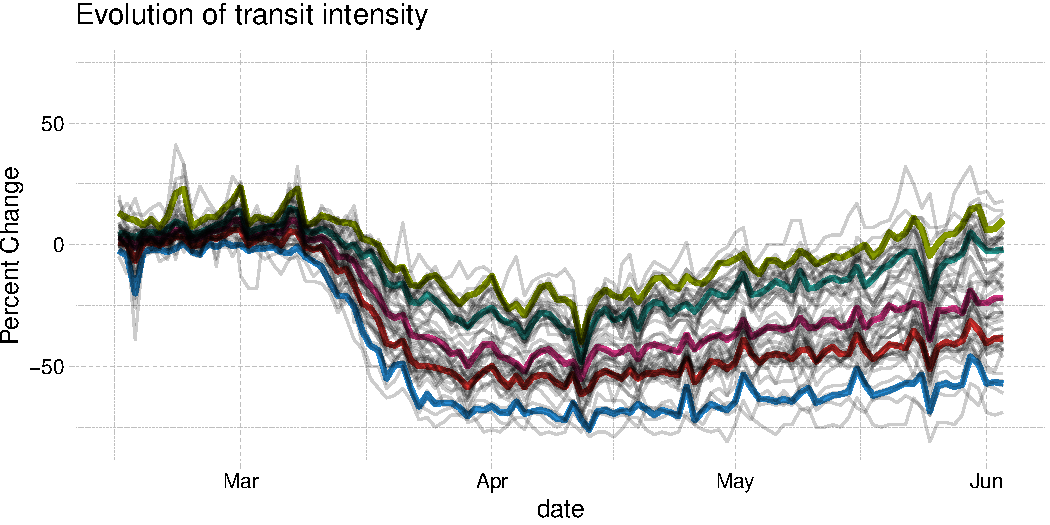
\includegraphics[width=0.5\linewidth]{tables_and_figures/transit}
      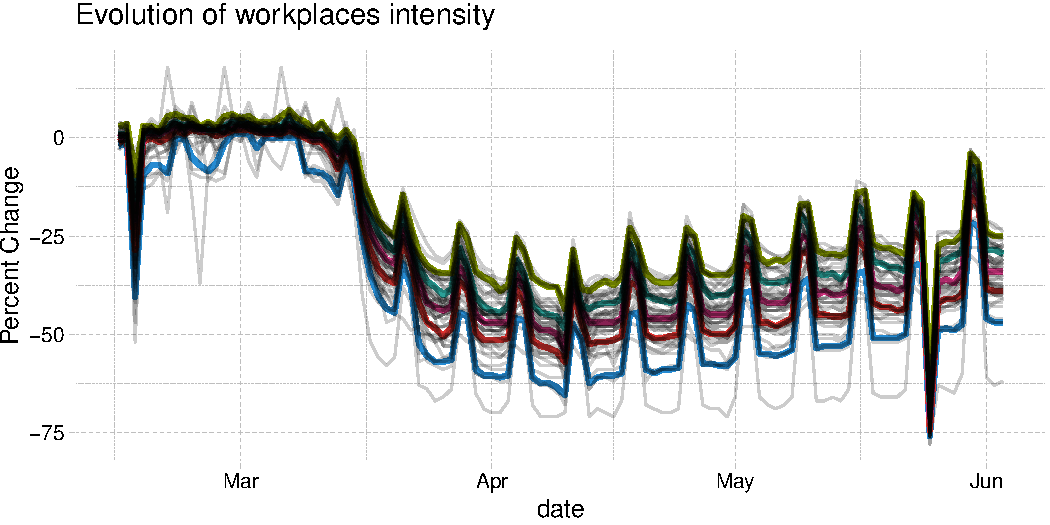
\includegraphics[width=0.5\linewidth]{tables_and_figures/workplaces}
       \end{tabular}
        \begin{flushleft}
        \scriptsize{This figure shows the evolution of ``Transit stations'' and  ``Workplaces'' of Google Mobility
      Reports. Thin gray lines are the value in each state and date. Thicker colored lines are
      quantiles of the variables conditional on date.}
      \end{flushleft}
\end{figure}



In our empirical analysis, we use weekly measures for cases, deaths,
and tests by summing up their daily measures from day \(t\) to
\(t-6\).  We focus on weekly cases and deaths because daily new cases and deaths are
affected by the timing of reporting and testing, and are quite
volatile as shown in Figure \ref{fig:dailycases} in the
appendix.  Aggregating to weekly new cases/deaths/tests smooths
out idiosyncratic daily noises as well as periodic fluctuations
associated with days of the week.
We also construct weekly policy and
behavior variables by taking 7 day moving averages from day \(t-14\) to
\(t-21\) for case growth, where the  delay reflects the time lag between infection and case confirmation. The four weekly behavior variables are referred as ``Transit
Intensity,'' ``Workplace Intensity,'' ``Retail Intensity,'' and ``Grocery
Intensity.'' Consequently, our empirical analysis uses 7 day moving averages of all variables recorded at daily frequencies. Our sample period is from March 7, 2020 to June 3, 2020.

\begin{table}\caption{Correlations among Policies and Behavior \label{tab:correlation}}\vspace{-0.2cm}
  \begin{minipage}{\linewidth}
    \resizebox{\linewidth}{!}{
      
\begin{tabular}{lccccccccccc}
\toprule
\rotatebox{90}{ } & \rotatebox{90}{workplaces} & \rotatebox{90}{retail} & \rotatebox{90}{grocery} & \rotatebox{90}{transit} & \rotatebox{90}{masks for employees} & \rotatebox{90}{closed K-12 schools} & \rotatebox{90}{stay at home} & \rotatebox{90}{closed movie theaters} & \rotatebox{90}{closed restaurants} & \rotatebox{90}{closed businesses} & \rotatebox{90}{ave of four policy vars}\\
\midrule
workplaces & 1.00 &  &  &  &  &  &  &  &  &  & \\
retail & 0.93 & 1.00 &  &  &  &  &  &  &  &  & \\
grocery & 0.75 & 0.83 & 1.00 &  &  &  &  &  &  &  & \\
transit & 0.89 & 0.92 & 0.83 & 1.00 &  &  &  &  &  &  & \\
masks for employees & -0.32 & -0.17 & -0.15 & -0.29 & 1.00 &  &  &  &  &  & \\
\addlinespace
closed K-12 schools & -0.91 & -0.79 & -0.55 & -0.72 & 0.43 & 1.00 &  &  &  &  & \\
stay at home & -0.69 & -0.69 & -0.70 & -0.71 & 0.28 & 0.62 & 1.00 &  &  &  & \\
closed movie theaters & -0.81 & -0.76 & -0.64 & -0.71 & 0.34 & 0.82 & 0.72 & 1.00 &  &  & \\
closed restaurants & -0.77 & -0.82 & -0.68 & -0.76 & 0.21 & 0.74 & 0.72 & 0.82 & 1.00 &  & \\
closed businesses & -0.65 & -0.68 & -0.68 & -0.64 & 0.08 & 0.56 & 0.76 & 0.68 & 0.71 & 1.00 & \\
\addlinespace
ave of four policy vars & -0.84 & -0.84 & -0.75 & -0.79 & 0.24 & 0.78 & 0.81 & 0.92 & 0.93 & 0.87 & 1.00\\
\bottomrule
\end{tabular}
    }\smallskip
       \begin{flushleft}
         \scriptsize
         Each off-diagonal entry reports a correlation coefficient of
         a pair of policy and behavior variables.
       \end{flushleft}
  \end{minipage}
\end{table}

Table \ref{tab:correlation} reports that weekly policy and behavior
variables are highly correlated with each other, except for the``masks
for employees'' policy.  High correlations may cause multicolinearity
problems and could limit our ability to separately identify the
effect of each policy or behavior variable on case growth, but this
does not prevent us from identifying the aggregate effect of all
policies and behavior variables on case or death growth.

Figure \ref{fig:policyportion} shows the portion of states that have
each policy in place at each date. For most policies, there is
considerable variation across states in the time in which the policies
are active. The one exception is K-12 school closures. About 80\% of
states closed schools within a day or two of March 15th, and all
states closed schools by early April. This makes the effect of school
closings difficult to separate from aggregate time series variation.

\begin{figure}[ht]\caption{Portion of states with each
    policy \label{fig:policyportion}}
  \begin{minipage}{\linewidth}
    \begin{tabular}{ccc}
      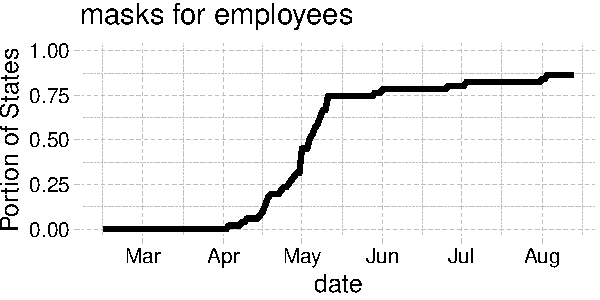
\includegraphics[width=0.31\textwidth]{tables_and_figures/pmaskbus_p}
      &
        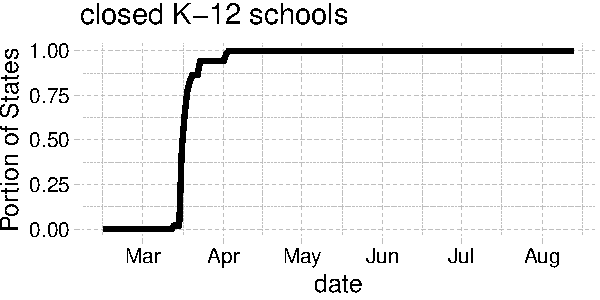
\includegraphics[width=0.31\textwidth]{tables_and_figures/pk12_p}
      &
        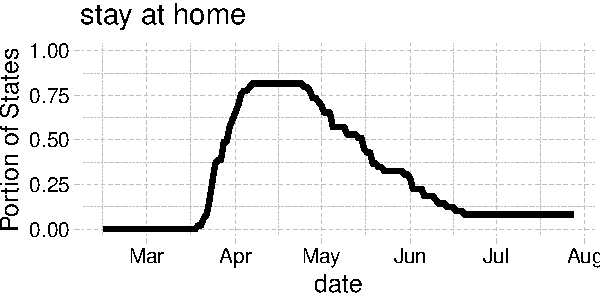
\includegraphics[width=0.31\textwidth]{tables_and_figures/pshelter_p}
      \\
      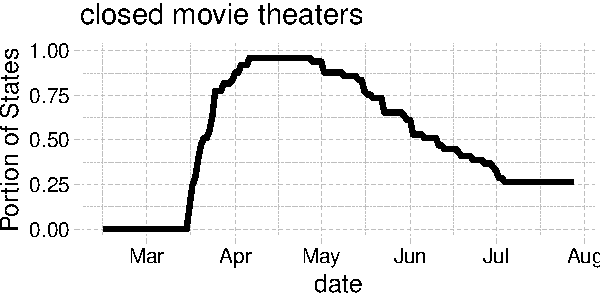
\includegraphics[width=0.31\textwidth]{tables_and_figures/pmovie_p}
      &
        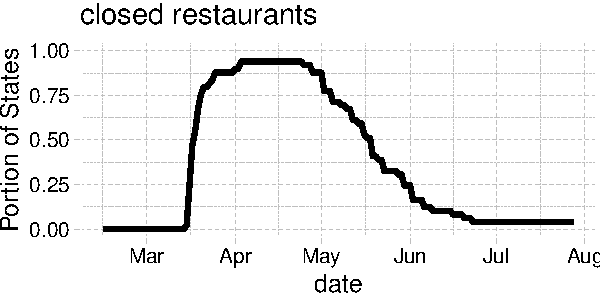
\includegraphics[width=0.31\textwidth]{tables_and_figures/prestaurant_p}
      &
        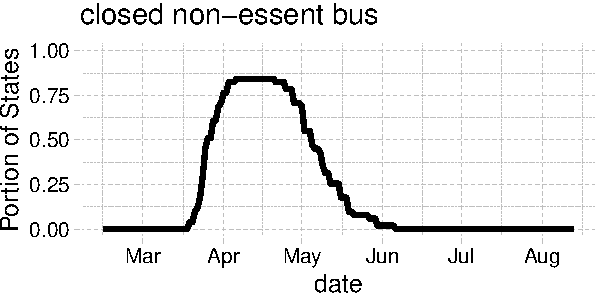
\includegraphics[width=0.31\textwidth]{tables_and_figures/pnonessential_p}
    \end{tabular}
  \end{minipage}
\end{figure}



\subsection{The Effect of Policies and Information on Behavior\label{policies-and-behavior}}

We first examine how policies and information affect social distancing behaviors by estimating a version of (\ref{eq:R2}):
\begin{align}
  {\bcolor B_{it}^j}
  %& = {\pcolor (\beta^j)' P_{it} }  + {\icolor \gamma_{1}^j \log(t) + \gamma_{2}^j \log (\Delta C_{i,t-14}) +  \gamma_{3}^j Y_{i,t-7}} + {\wcolor (\delta_B^j)' W_{it}} + \varepsilon_{it}^j \nonumber\\
  & = {\pcolor (\beta^j)' P_{it}} + {\icolor (\gamma^j)' I_{it}} +
    {\wcolor (\delta_B^j)' W_{it}} + \varepsilon_{it}^{bj}, \notag
\end{align}
where ${\bcolor B_{it}^j}$ represents behavior variable $j$  in state  $i$ at time $t$.
${\pcolor P_{it}}$ collects the Covid related policies  in state $i$ at $t$.
Confounders, ${\wcolor W_{it}}$, include state-level covariates, month
indicators, and their interactions.
${\icolor I_{it}}$ is a set of information variables that affect
people's behaviors at $t$. As information, we include each state's
growth of cases (in panel \ref{tab:PItoBcases}) or deaths (in panel
\ref{tab:PItoBdeaths}), and log cases or deaths.  Additionally, in
columns (5)-(8) of each panel, we include national growth and log
of cases or deaths.

\afterpage{\clearpage
  %\thispagestyle{empty}
  \begin{landscape}
    \begin{table}[!htbp] \centering
      \caption{The Effect of Policies and Information on Behavior ($P
        I \to B$)}\vspace{-0.3cm}\label{tab:PItoB}

      \begin{subtable}{\linewidth}\caption{Cases as Information\label{tab:PItoBcases}}
      \begin{minipage}{\linewidth}
        \centering
        \resizebox{\textwidth}{!}{
          \footnotesize
          \begin{tabular}{@{\extracolsep{1pt}}lcccccccc} 
\\[-1.8ex]\hline 
\hline \\[-1.8ex] 
 & \multicolumn{8}{c}{\textit{Dependent variable:}} \\ 
\cline{2-9} 
 & workplaces & retail & grocery & transit & workplaces & retail & grocery & transit \\ 
\\[-1.8ex] & (1) & (2) & (3) & (4) & (5) & (6) & (7) & (8)\\ 
\hline \\[-1.8ex] 
 masks for employees & 0.0003 & $-$0.008 & $-$0.025$^{***}$ & $-$0.033 & $-$0.006 & $-$0.018$^{*}$ & $-$0.026$^{***}$ & $-$0.041$^{**}$ \\ 
  & (0.007) & (0.012) & (0.009) & (0.021) & (0.005) & (0.011) & (0.009) & (0.020) \\ 
  closed K-12 schools & $-$0.187$^{***}$ & $-$0.201$^{***}$ & $-$0.128$^{***}$ & $-$0.214$^{***}$ & $-$0.055$^{***}$ & $-$0.029$^{*}$ & $-$0.089$^{***}$ & $-$0.063$^{*}$ \\ 
  & (0.022) & (0.034) & (0.021) & (0.046) & (0.011) & (0.017) & (0.026) & (0.038) \\ 
  stay at home & $-$0.010 & $-$0.025$^{*}$ & $-$0.041$^{***}$ & $-$0.051$^{**}$ & $-$0.017$^{*}$ & $-$0.037$^{***}$ & $-$0.041$^{***}$ & $-$0.059$^{**}$ \\ 
  & (0.010) & (0.013) & (0.014) & (0.024) & (0.009) & (0.011) & (0.014) & (0.024) \\ 
  closed movie theaters & $-$0.012 & $-$0.022 & $-$0.021$^{**}$ & 0.021 & $-$0.009 & $-$0.021$^{*}$ & $-$0.019$^{*}$ & 0.024 \\ 
  & (0.010) & (0.014) & (0.011) & (0.023) & (0.008) & (0.012) & (0.010) & (0.022) \\ 
  closed restaurants & $-$0.021$^{***}$ & $-$0.063$^{***}$ & $-$0.008 & $-$0.065$^{***}$ & $-$0.009 & $-$0.044$^{***}$ & $-$0.006 & $-$0.052$^{**}$ \\ 
  & (0.007) & (0.012) & (0.007) & (0.024) & (0.006) & (0.009) & (0.006) & (0.023) \\ 
  closed businesses & $-$0.022$^{**}$ & $-$0.022$^{**}$ & $-$0.026$^{**}$ & $-$0.018 & $-$0.023$^{***}$ & $-$0.025$^{***}$ & $-$0.025$^{**}$ & $-$0.019 \\ 
  & (0.009) & (0.010) & (0.011) & (0.021) & (0.008) & (0.008) & (0.010) & (0.020) \\ 
  $\Delta \log \Delta C_{it}$ & 0.019$^{***}$ & 0.014$^{***}$ & 0.020$^{***}$ & 0.019$^{***}$ & 0.018$^{***}$ & 0.015$^{***}$ & 0.017$^{***}$ & 0.017$^{***}$ \\ 
  & (0.003) & (0.005) & (0.004) & (0.005) & (0.002) & (0.003) & (0.004) & (0.006) \\ 
  $\log \Delta C_{it}$ & $-$0.028$^{***}$ & $-$0.031$^{***}$ & $-$0.002 & $-$0.020$^{**}$ & $-$0.010$^{***}$ & $-$0.010 & 0.005 & 0.0001 \\ 
  & (0.004) & (0.007) & (0.004) & (0.010) & (0.003) & (0.007) & (0.005) & (0.012) \\ 
  $\Delta \log \Delta C_{it}$.national &  &  &  &  & $-$0.024$^{***}$ & $-$0.061$^{***}$ & 0.012$^{**}$ & $-$0.024$^{**}$ \\ 
  &  &  &  &  & (0.004) & (0.007) & (0.006) & (0.010) \\ 
  $\log \Delta C_{it}$.national &  &  &  &  & $-$0.059$^{***}$ & $-$0.077$^{***}$ & $-$0.017$^{**}$ & $-$0.068$^{***}$ \\ 
  &  &  &  &  & (0.004) & (0.008) & (0.008) & (0.012) \\ 
 \hline \\[-1.8ex] 
state variables & Yes & Yes & Yes & Yes & Yes & Yes & Yes & Yes \\ 
Month $\times$ state variables & Yes & Yes & Yes & Yes & Yes & Yes & Yes & Yes \\ 
\hline \\[-1.8ex] 
$\sum_j \mathrm{Policy}_j$ & -0.251$^{***}$ & -0.341$^{***}$ & -0.249$^{***}$ & -0.361$^{***}$ & -0.119$^{***}$ & -0.174$^{***}$ & -0.206$^{***}$ & -0.208$^{***}$ \\ 
 & (0.027) & (0.044) & (0.031) & (0.062) & (0.016) & (0.024) & (0.032) & (0.047) \\ 
Observations & 4,400 & 4,400 & 4,400 & 4,400 & 4,400 & 4,400 & 4,400 & 4,400 \\ 
R$^{2}$ & 0.928 & 0.885 & 0.803 & 0.829 & 0.955 & 0.921 & 0.808 & 0.848 \\ 
Adjusted R$^{2}$ & 0.927 & 0.884 & 0.802 & 0.828 & 0.955 & 0.920 & 0.807 & 0.847 \\ 
\hline 
\hline \\[-1.8ex] 
\textit{Note:}  & \multicolumn{8}{r}{$^{*}$p$<$0.1; $^{**}$p$<$0.05; $^{***}$p$<$0.01} \\ 
\end{tabular} 
        }
      \begin{flushleft}
        \scriptsize
        Dependent variables are   ``Transit
        Intensity,'' ``Workplace Intensity,'' ``Retail Intensity,'' and ``Grocery
        Intensity" defined as 7 days moving averages of corresponding daily measures obtained from Google Mobility Reports.  All specifications include state-level characteristics (population, area, unemployment rate, poverty rate, and a percentage of people subject to illness) as well as their interactions with the log of days since Jan 15, 2020. The row ``$\sum_j \text{Policy}_j$'' reports the sum of six policy coefficients. Standard errors are clustered at the state level.
        \end{flushleft}
      \end{minipage}
    \end{subtable}
  \end{table}
  \pagebreak
  \begin{table}[!htbp] \centering
    \ContinuedFloat
    \begin{subtable}{\linewidth}\caption{Deaths as Information \label{tab:PItoBdeaths}}
      \begin{minipage}{\linewidth}
        \centering
        \resizebox{\textwidth}{!}{
          \footnotesize
            \begin{tabular}{@{\extracolsep{1pt}}lcccccccc} 
\\[-1.8ex]\hline 
\hline \\[-1.8ex] 
 & \multicolumn{8}{c}{\textit{Dependent variable:}} \\ 
\cline{2-9} 
 & workplaces & retail & grocery & transit & workplaces & retail & grocery & transit \\ 
\\[-1.8ex] & (1) & (2) & (3) & (4) & (5) & (6) & (7) & (8)\\ 
\hline \\[-1.8ex] 
 masks for employees & $-$0.007 & $-$0.023$^{*}$ & $-$0.033$^{***}$ & $-$0.047$^{**}$ & $-$0.015$^{**}$ & $-$0.034$^{**}$ & $-$0.037$^{***}$ & $-$0.055$^{**}$ \\ 
  & (0.007) & (0.014) & (0.010) & (0.023) & (0.006) & (0.013) & (0.009) & (0.023) \\ 
  closed K-12 schools & $-$0.243$^{***}$ & $-$0.262$^{***}$ & $-$0.126$^{***}$ & $-$0.249$^{***}$ & $-$0.054$^{***}$ & $-$0.018 & $-$0.039$^{*}$ & $-$0.048 \\ 
  & (0.022) & (0.031) & (0.017) & (0.038) & (0.017) & (0.019) & (0.024) & (0.047) \\ 
  closed movie theaters & $-$0.023$^{**}$ & $-$0.041$^{**}$ & $-$0.031$^{***}$ & 0.002 & $-$0.012 & $-$0.027$^{**}$ & $-$0.026$^{**}$ & 0.014 \\ 
  & (0.011) & (0.016) & (0.011) & (0.023) & (0.008) & (0.013) & (0.011) & (0.023) \\ 
  stay at home & $-$0.024$^{**}$ & $-$0.053$^{***}$ & $-$0.058$^{***}$ & $-$0.084$^{***}$ & $-$0.027$^{***}$ & $-$0.058$^{***}$ & $-$0.059$^{***}$ & $-$0.087$^{***}$ \\ 
  & (0.009) & (0.014) & (0.014) & (0.024) & (0.009) & (0.012) & (0.014) & (0.025) \\ 
  closed restaurants & $-$0.033$^{***}$ & $-$0.078$^{***}$ & $-$0.012 & $-$0.080$^{***}$ & $-$0.014$^{**}$ & $-$0.052$^{***}$ & $-$0.002 & $-$0.060$^{**}$ \\ 
  & (0.010) & (0.015) & (0.007) & (0.025) & (0.007) & (0.011) & (0.006) & (0.024) \\ 
  closed businesses & $-$0.022$^{**}$ & $-$0.025$^{*}$ & $-$0.028$^{**}$ & $-$0.019 & $-$0.011 & $-$0.011 & $-$0.022$^{**}$ & $-$0.007 \\ 
  & (0.010) & (0.014) & (0.011) & (0.021) & (0.009) & (0.012) & (0.010) & (0.020) \\ 
  $\Delta \log \Delta D_{it}$ & $-$0.009$^{**}$ & $-$0.021$^{***}$ & $-$0.006 & $-$0.014$^{**}$ & 0.001 & $-$0.003 & 0.0003 & $-$0.002 \\ 
  & (0.004) & (0.006) & (0.004) & (0.006) & (0.002) & (0.004) & (0.004) & (0.006) \\ 
  $\log \Delta D_{it}$ & $-$0.010$^{**}$ & $-$0.001 & 0.002 & 0.001 & $-$0.006 & 0.002 & 0.003 & 0.005 \\ 
  & (0.004) & (0.008) & (0.006) & (0.012) & (0.004) & (0.008) & (0.006) & (0.013) \\ 
  $\Delta \log \Delta D_{it}$.national &  &  &  &  & $-$0.039$^{***}$ & $-$0.066$^{***}$ & $-$0.022$^{***}$ & $-$0.044$^{***}$ \\ 
  &  &  &  &  & (0.003) & (0.006) & (0.004) & (0.008) \\ 
  $\log \Delta D_{it}$.national &  &  &  &  & $-$0.064$^{***}$ & $-$0.080$^{***}$ & $-$0.029$^{***}$ & $-$0.067$^{***}$ \\ 
  &  &  &  &  & (0.004) & (0.006) & (0.006) & (0.010) \\ 
 \hline \\[-1.8ex] 
state variables & Yes & Yes & Yes & Yes & Yes & Yes & Yes & Yes \\ 
Month $\times$ state variables & Yes & Yes & Yes & Yes & Yes & Yes & Yes & Yes \\ 
\hline \\[-1.8ex] 
$\sum_j \mathrm{Policy}_j$ & -0.354$^{***}$ & -0.482$^{***}$ & -0.286$^{***}$ & -0.478$^{***}$ & -0.133$^{***}$ & -0.200$^{***}$ & -0.186$^{***}$ & -0.243$^{***}$ \\ 
 & (0.022) & (0.036) & (0.030) & (0.058) & (0.021) & (0.031) & (0.033) & (0.059) \\ 
Observations & 4,400 & 4,400 & 4,400 & 4,400 & 4,400 & 4,400 & 4,400 & 4,400 \\ 
R$^{2}$ & 0.899 & 0.847 & 0.773 & 0.800 & 0.941 & 0.902 & 0.788 & 0.825 \\ 
Adjusted R$^{2}$ & 0.898 & 0.846 & 0.772 & 0.799 & 0.941 & 0.901 & 0.787 & 0.824 \\ 
\hline 
\hline \\[-1.8ex] 
\textit{Note:}  & \multicolumn{8}{r}{$^{*}$p$<$0.1; $^{**}$p$<$0.05; $^{***}$p$<$0.01} \\ 
\end{tabular} 
          }
        \begin{flushleft}
          \scriptsize
          Dependent variables are   ``Transit
          Intensity,'' ``Workplace Intensity,'' ``Retail Intensity,'' and ``Grocery
          Intensity" defined as 7 days moving averages of corresponding daily measures obtained from Google Mobility Reports.  All specifications include state-level characteristics (population, area, unemployment rate, poverty rate, and a percentage of people subject to illness) as well as their interactions with the log of days since Jan 15, 2020. The row ``$\sum_j \text{Policy}_j$'' reports the sum of six policy coefficients. Standard errors are clustered at the state level.
        \end{flushleft}
      \end{minipage}
    \end{subtable}
  \end{table}
\end{landscape}
\clearpage}

Table \ref{tab:PItoB} reports the estimates with standard errors clustered at the state level.  Across different
specifications, our results imply that policies have large effects on
behavior. Comparing columns (1)-(4) with columns (5)-(8),
the magnitude of policy effects are sensitive to whether national
cases or deaths are included as information. The coefficient on school
closures is particularly sensitive to the inclusion of national
information variables.  As shown in Figure
\ref{fig:policyportion}, there is little variation across states in
the timing of school closures. Consequently, it is difficult to
separate the effect of school closures from a behavioral response to the national
trend in cases and deaths.

The other policy coefficients are less sensitive to the inclusion of
national case/death variables. After school closures, stay-at-home
orders and restaurant closures have the next largest effect. Somewhat
surprisingly, closure of nonessential businesses appears to have
a modest effect on behavior. Closing movie theaters has a similar,
small effect on behavior. The effect of masks for employees is also
small. The comparison of effects across policies should be interpreted
with caution.  Differences between policy effects are often
statistically insignificant; except for masks for employees, the
policies are highly correlated and it is difficult to separate their
effects.


The row ``$\sum_j \mathrm{Policy}_j$'' reports the sum of the estimated
effect of all policies, which is substantial and can account for a
large fraction of the observed declines in behavior variables.  For
example,  in Figure \ref{fig:transit-workplaces}, transit intensity for a median state was approximately -50\% at its lowest point
 in early April. The estimated policy coefficients in columns imply
that imposing all six policies would lead to roughly 85\% (in columns
1-4) or roughly 50\% (in columns 5-8) of the observed decline. The large impact of policies on transit intensity suggests that the policies may have reduced the Covid-19 infection by reducing people's use of public transportation.\footnote{Analyzing the New York City's subway ridership,  \cite{NBERw27021} finds  a strong link between public transit and spread of infection.}


%retail intensity was approximately -40\% at its lowest point
%in mid April, and the estimated policy coefficients in columns imply
%that imposing all six policies would lead to either all (in columns
%1-4) or half (in columns 5-8) of the observed decline.

In panel \ref{tab:PItoBdeaths}, estimated coefficients of deaths and
death growth are generally negative. This suggests that the higher
number of deaths reduces social interactions measured by Google
Mobility Reports perhaps because people are increasingly aware of
prevalence of Covid-19 \citep{maloney2020}.  The coefficients on log
cases and case growth in panel \ref{tab:PItoBcases} are more mixed. In
columns (5)-(8) of both panels, we see that national case/death
variables have large, negative coefficients. This suggests that behavior responded to national conditions although it is also likely that national case/death variables capture unobserved aggregate time effects beyond information (e.g., latent policy variables and time-varying confounders that are common across states) which are not fully controlled by month dummies.


%For grocery, the positive estimated coefficients of cases and case growth in columns (3) and (7) might be capturing stockpiling behavior, which could temporarily increase the visits to grocery.


%In columns (5)-(8), the effects of masks for employees are allowed to be different before and after May 1st. The negative effect of mask mandates on mobility measures appears to be slightly larger in May than in April but the difference is not statistically significant.

\begin{figure}[ht]
  \caption{Case and death growth conditional on mask mandates \label{fig:masks}}\vspace{0.2cm}
 \begin{minipage}{\linewidth}
    \centering
    \begin{tabular}{cc}
      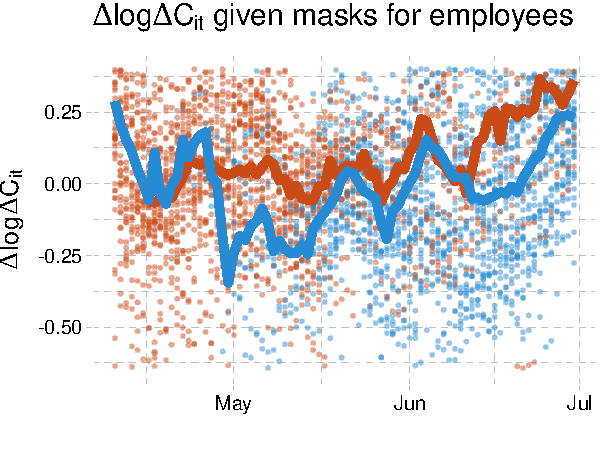
\includegraphics[width=0.5\textwidth]{tables_and_figures/pmaskbus-cases-14}
      &
        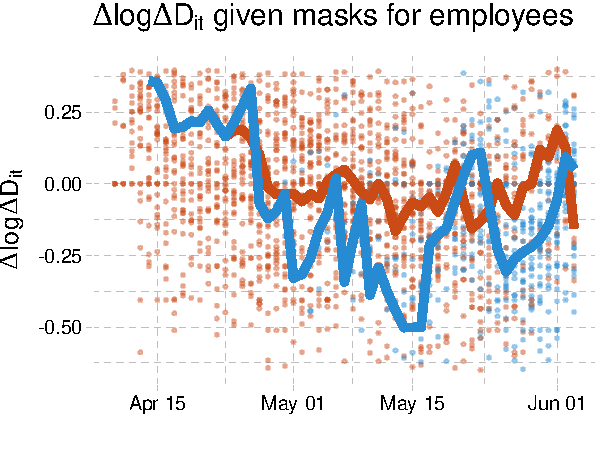
\includegraphics[width=0.5\textwidth]{tables_and_figures/pmaskbus-deaths-21}
    \end{tabular}
    \begin{flushleft}
      \scriptsize In these figures, red points are the case or death
      growth rate in states without a mask mandate. Blue points are
      states with a mask mandate 14 (21 for deaths) days prior. The
      red line is the average across states without a mask mandate 14
      (21 for deaths) days earlier. The blue line is the average
      across states with a mask mandate 14 (21 for deaths) earlier.
    \end{flushleft}
  \end{minipage}
\end{figure}



\afterpage{
 \clearpage
 %\thispagestyle{empty}
 \begin{landscape}
\begin{table}[!htbp] \centering
 \caption{The Direct Effect of Behavior and Policies on Case and
   Death Growth ($BPI \to Y$)}\vspace{-0.3cm}
 \label{tab:BPItoY}
 \begin{minipage}{\linewidth}
   \centering
   \resizebox{\textwidth}{!}{
   \tiny
   \begin{tabular}{c|c}
   \begin{minipage}{0.49\linewidth}
     \centering
     \begin{tabular}{@{\extracolsep{1pt}}lcccc} 
\\[-1.8ex]\hline 
\hline \\[-1.8ex] 
 & \multicolumn{4}{c}{\textit{Dependent variable:}} \\ 
\cline{2-5} 
 & \multicolumn{4}{c}{$\Delta \log \Delta C_{it}$} \\ 
\\[-1.8ex] & (1) & (2) & (3) & (4)\\ 
\hline \\[-1.8ex] 
 lag(masks for employees, 14) & $-$0.093$^{***}$ &  & $-$0.108$^{***}$ &  \\ 
  & (0.036) &  & (0.033) &  \\ 
  lag(masks*April, 14) &  & $-$0.145$^{***}$ &  & $-$0.169$^{***}$ \\ 
  &  & (0.052) &  & (0.051) \\ 
  lag(masks*May, 14) &  & $-$0.080$^{**}$ &  & $-$0.093$^{***}$ \\ 
  &  & (0.039) &  & (0.036) \\ 
  lag(closed K-12 schools, 14) & $-$0.127 & $-$0.134 & $-$0.006 & $-$0.012 \\ 
  & (0.090) & (0.089) & (0.106) & (0.105) \\ 
  lag(closed movie theaters, 14) & 0.039 & 0.035 & 0.050 & 0.045 \\ 
  & (0.050) & (0.050) & (0.047) & (0.047) \\ 
  lag(stay at home, 14) & $-$0.082$^{*}$ & $-$0.087$^{*}$ & $-$0.100$^{**}$ & $-$0.105$^{**}$ \\ 
  & (0.049) & (0.050) & (0.050) & (0.051) \\ 
  lag(closed restaurants, 14) & 0.015 & 0.015 & 0.015 & 0.014 \\ 
  & (0.045) & (0.045) & (0.044) & (0.044) \\ 
  lag(closed businesses, 14) & $-$0.007 & $-$0.003 & $-$0.027 & $-$0.023 \\ 
  & (0.042) & (0.041) & (0.040) & (0.040) \\ 
  lag(workplaces, 14) & 0.852 & 0.836 & 0.111 & 0.085 \\ 
  & (0.571) & (0.565) & (0.628) & (0.617) \\ 
  lag(retail, 14) & 0.497 & 0.464 & 0.124 & 0.085 \\ 
  & (0.337) & (0.347) & (0.355) & (0.364) \\ 
  lag(grocery, 14) & $-$0.592$^{**}$ & $-$0.607$^{**}$ & $-$0.282 & $-$0.298 \\ 
  & (0.292) & (0.293) & (0.280) & (0.280) \\ 
  lag(transit, 14) & 0.551$^{*}$ & 0.558$^{*}$ & 0.541$^{**}$ & 0.548$^{**}$ \\ 
  & (0.288) & (0.287) & (0.275) & (0.274) \\ 
  lag($\Delta \log \Delta C_{it}$, 14) & 0.013 & 0.013 & 0.030 & 0.030 \\ 
  & (0.026) & (0.026) & (0.028) & (0.028) \\ 
  lag($\log \Delta C_{it}$, 14) & $-$0.111$^{***}$ & $-$0.112$^{***}$ & $-$0.096$^{***}$ & $-$0.096$^{***}$ \\ 
  & (0.023) & (0.023) & (0.027) & (0.028) \\ 
  lag($\Delta \log \Delta C_{it}$.national, 14) &  &  & $-$0.126$^{***}$ & $-$0.126$^{***}$ \\ 
  &  &  & (0.041) & (0.041) \\ 
  lag($\log \Delta C_{it}$.national, 14) &  &  & $-$0.204$^{***}$ & $-$0.205$^{***}$ \\ 
  &  &  & (0.049) & (0.049) \\ 
  $\Delta \log T_{it}$ & 0.138$^{***}$ & 0.139$^{***}$ & 0.141$^{***}$ & 0.141$^{***}$ \\ 
  & (0.043) & (0.043) & (0.041) & (0.041) \\ 
 \hline \\[-1.8ex] 
state variables & Yes & Yes & Yes & Yes \\ 
Month $\times$ state variables & Yes & Yes & Yes & Yes \\ 
\hline \\[-1.8ex] 
$\sum_j \mathrm{Policy}_j$ & -0.255$^{*}$ & -0.400$^{**}$ & -0.175 & -0.343$^{*}$ \\ 
 & (0.138) & (0.156) & (0.161) & (0.176) \\ 
$\sum_k w_k \mathrm{Behavior}_k$ & -0.734$^{***}$ & -0.713$^{***}$ & -0.292$^{*}$ & -0.265$^{*}$ \\ 
 & (0.160) & (0.162) & (0.158) & (0.155) \\ 
Observations & 3,624 & 3,624 & 3,624 & 3,624 \\ 
R$^{2}$ & 0.765 & 0.766 & 0.772 & 0.772 \\ 
Adjusted R$^{2}$ & 0.763 & 0.763 & 0.769 & 0.769 \\ 
\hline 
\hline \\[-1.8ex] 
\textit{Note:}  & \multicolumn{4}{r}{$^{*}$p$<$0.1; $^{**}$p$<$0.05; $^{***}$p$<$0.01} \\ 
\end{tabular} 
   \end{minipage}
     %\hspace{1pt}
     &
   \begin{minipage}{0.49\linewidth}
     \centering
     \begin{tabular}{@{\extracolsep{1pt}}lcccc} 
\\[-1.8ex]\hline 
\hline \\[-1.8ex] 
 & \multicolumn{4}{c}{\textit{Dependent variable:}} \\ 
\cline{2-5} 
 & \multicolumn{4}{c}{$\Delta \log \Delta D_{it}$} \\ 
\\[-1.8ex] & (1) & (2) & (3) & (4)\\ 
\hline \\[-1.8ex] 
 lag(masks for employees, 21) & $-$0.068$^{*}$ & $-$0.071$^{*}$ & $-$0.076$^{**}$ & $-$0.079$^{**}$ \\ 
  & (0.037) & (0.040) & (0.038) & (0.040) \\ 
  lag(closed K-12 schools, 21) & $-$0.306$^{***}$ & $-$0.313$^{***}$ & $-$0.215$^{**}$ & $-$0.223$^{**}$ \\ 
  & (0.104) & (0.103) & (0.104) & (0.104) \\ 
  lag(stay at home, 21) & 0.024 & 0.024 & 0.019 & 0.020 \\ 
  & (0.047) & (0.043) & (0.047) & (0.044) \\ 
  lag(business closure policies, 21) & 0.031 &  & 0.030 &  \\ 
  & (0.070) &  & (0.070) &  \\ 
  lag(closed movie theaters, 21) &  & $-$0.007 &  & $-$0.003 \\ 
  &  & (0.052) &  & (0.051) \\ 
  lag(closed restaurants, 21) &  & 0.040 &  & 0.033 \\ 
  &  & (0.053) &  & (0.052) \\ 
  lag(closed non-essent bus, 21) &  & $-$0.006 &  & $-$0.004 \\ 
  &  & (0.041) &  & (0.042) \\ 
  lag(workplaces, 21) & 1.504$^{***}$ & 1.481$^{***}$ & 1.208$^{**}$ & 1.200$^{**}$ \\ 
  & (0.510) & (0.503) & (0.516) & (0.514) \\ 
  lag(retail, 21) & 0.167 & 0.199 & 0.035 & 0.060 \\ 
  & (0.377) & (0.386) & (0.354) & (0.361) \\ 
  lag(grocery, 21) & $-$0.491 & $-$0.526 & $-$0.436 & $-$0.463 \\ 
  & (0.358) & (0.369) & (0.338) & (0.346) \\ 
  lag(transit, 21) & 0.091 & 0.104 & 0.117 & 0.126 \\ 
  & (0.147) & (0.141) & (0.146) & (0.141) \\ 
  lag($\Delta \log \Delta D_{it}$, 21) & 0.039 & 0.038 & 0.043 & 0.043 \\ 
  & (0.035) & (0.035) & (0.037) & (0.038) \\ 
  lag($\log \Delta D_{it}$, 21) & $-$0.061$^{***}$ & $-$0.059$^{***}$ & $-$0.059$^{***}$ & $-$0.058$^{***}$ \\ 
  & (0.017) & (0.018) & (0.017) & (0.018) \\ 
  lag($\Delta \log \Delta D_{it}$.national, 21) &  &  & $-$0.067 & $-$0.067 \\ 
  &  &  & (0.047) & (0.047) \\ 
  lag($\log \Delta D_{it}$.national, 21) &  &  & $-$0.051 & $-$0.049 \\ 
  &  &  & (0.031) & (0.031) \\ 
   &  &  &  &  \\ 
  &  &  &  &  \\ 
 \hline \\[-1.8ex] 
state variables & Yes & Yes & Yes & Yes \\ 
Month $\times$ state variables & Yes & Yes & Yes & Yes \\ 
\hline \\[-1.8ex] 
$\sum_j \mathrm{Policy}_j$ & -0.319$^{**}$ & -0.333$^{**}$ & -0.242$^{*}$ & -0.256$^{*}$ \\ 
 & (0.132) & (0.136) & (0.130) & (0.135) \\ 
$\sum_k w_k \mathrm{Behavior}_k$ & -0.707$^{***}$ & -0.711$^{***}$ & -0.539$^{***}$ & -0.547$^{***}$ \\ 
 & (0.151) & (0.153) & (0.152) & (0.156) \\ 
Observations & 4,845 & 4,845 & 4,845 & 4,845 \\ 
R$^{2}$ & 0.451 & 0.451 & 0.452 & 0.452 \\ 
Adjusted R$^{2}$ & 0.447 & 0.447 & 0.448 & 0.448 \\ 
\hline 
\hline \\[-1.8ex] 
\textit{Note:}  & \multicolumn{4}{r}{$^{*}$p$<$0.1; $^{**}$p$<$0.05; $^{***}$p$<$0.01} \\ 
\end{tabular} 
   \end{minipage}
   \end{tabular}
   }
 \begin{flushleft}
     \scriptsize Dependent variable is the weekly growth rate of
     confirmed cases (in the left panel) or deaths (in the right
     panel) as defined in equation (\ref{eq:y}). The covariates
     include lagged policy and behavior variables, which are
     constructed as 7 day moving averages between $t$ to $t-7$ of
     corresponding daily measures.  The row
     ``$\sum_j \mathrm{Policies}_j$'' reports the sum of six policy
     coefficients.  The row ``$\sum_k w_k \mathrm{Behavior}_k$''
     reports the sum of four coefficients of behavior variables
     weighted by the average of each behavioral variable from April
     1st-10th.  Standard errors are clustered at the state level.
   \end{flushleft}
 \end{minipage}
\end{table}
\end{landscape}
\clearpage
}

\subsection{The Direct Effect of Policies and Behavior on Case
and Death Growth\label{policy-behavior-and-case-growth}}

We now analyze how behavior and policies together influence case and death
growth rates. We begin with some simple graphical evidence of the
effect of policies on case and death growth. Figure \ref{fig:masks}
shows average case and death growth conditional on date and whether
masks are mandatory for employees.\footnote{We take 14 and 21 day lags of mask policies for case and death growths, respectively, to  identify the states with a mask mandate because policies affect cases and deaths with time lags. See our discussion in the Appendix \ref{sec:timing}.  } The left panel of the figure shows
that states with a mask mandate consistently have 0-0.2 lower case
growth than states without. The right panel  also illustrates that
states with a mask mandate tend to have lower average death growth than states without a mask mandate.

Similar plots are shown for other policies in Figures
\ref{fig:growthpolicies1} and \ref{fig:growthpolicies2} in the
appendix. The  figures for stay-at-home orders and closure
of nonessential businesses are qualitatively similar to that for
masks. States with these two policies appear to have about 0.1 percentage point lower
case growth  than states without. The effects of school closures, movie theater closures, and
restaurant closures are not clearly visible in these figures. These
figures are merely suggestive; the patterns observed in them may be
driven by confounders.

We more formally analyze the effect of policies by estimating
regressions. We first look at the direct effect of policies on case and death growth
conditional on behavior by estimating equation (\ref{eq:R1}):
% We partition $X_{it}$ in (\ref{eq:M}) into behavior variables $B_{it}$,  policy variables $P_{it}$, information variables $I_{it}$, and other confounding variables $W_{X,it}$ as $X_{it}= (B_{it}',P_{it}', I_{it}', W_{X,it}')'$ with $\theta=(\alpha',\pi',\mu',\delta_X')'$ and rewrite  (\ref{eq:M}) as:
\begin{align}
  {\ycolor  Y_{i,t+\ell}}
  & = {\bcolor \alpha ' B_{it}} + {\pcolor\pi 'P_{it}} + {\icolor \mu'I_{it}} +  {\wcolor\delta_Y 'W_{it}}  + \varepsilon^y_{it},
  \label{eq:reg-y}
\end{align}
where the outcome variable, $\ycolor Y_{i,t+\ell}$, is either case growth  or death growth.

For case growth as the outcome, we choose a lag length of $\ell=14$ days for behavior, policy, and information variables to reflect the delay between infection and
confirmation of case.\footnote{As we review in the Appendix \ref{sec:timing},
  a lag length of 14 days between exposure and case reporting, as well as a lag length of 21 days between exposure and deaths, is broadly consistent with currently
  available evidence.  }   $\bcolor B_{it}=(B_{it}^1,...,B_{it}^4)'$ is a vector of four behavior
variables  in state $i$. $\pcolor P_{it}$ includes the Covid-related policies
in state $i$  that directly affect the spread of Covid-19
after controlling for behavior variables (e.g., masks for employees).
We include information variables,  $\icolor I_{it}$, that include the past cases and case growths
because  the past cases may be
correlated with (latent) government  policies or people's behaviors
that are not fully captured by our observed policy and behavior
variables. We also consider a specification that includes the past cases and case growth at the national level as additional information variables. $\wcolor W_{it}$ is a set of confounders that include month dummies, state-level covariates,  and the interaction terms between month dummies and state-level covariates.\footnote{Month dummies also represent the latent information that is not fully captured by the past cases and growths.}
For case growth, $\wcolor W_{it}$ also includes the  test rate growth  $\Delta \log(T)_{it}$  to capture the effect of changing test rates on confirmed cases.
Equation (\ref{eq:reg-y}) corresponds to (\ref{eq:M})  derived from the SIR model.

%We also estimate the effect of policies on death growth by estimating  (\ref{eq:reg-y}) with death growth
%$\Delta \log \Delta D_{it}$  as outcome variable.
For death growth as the outcome, we take a lag length of $\ell=21$ days. The information variables $\icolor I_{it}$ include  past deaths and death growth rates;  $\wcolor W_{it}$ is the same as that of the case growth equation except that the growth rate of test rates is excluded from $\wcolor W_{it}$ as implied by equation (\ref{eq:M-D}).



% Tables \ref{tab:BPItoY-c} and  \ref{tab:BPItoY-d} show
Table \ref{tab:BPItoY} shows
the results of estimating
(\ref{eq:reg-y}) for case and death growth rates. %, respectively.
Column (1) represents our baseline specification while column (2) allows the effect of masks to be different before and after May 1st. Columns (3) and (4) include past cases/deaths and growth rates at national level as additional regressors.

The estimates indicate that mandatory face masks for employees
reduce the growth rate of infections and deaths by 8-15 percent, while holding behavior constant. This suggests that
requiring masks for employees in public-facing businesses may be an effective preventive measure.\footnote{Note that we are \textit{not} evaluating the effect of \textit{universal} mask-wearing for the public but that of mask-wearing for employees. The effect of \textit{universal} mask-wearing for the public could be larger if people comply with such a policy measure. \cite{tian2020calibrated} considered a  model in which mask wearing reduces  the reproduction number by a factor $(1-e \cdot pm)^2$, where $e$ is the efficacy of trapping viral particles inside the mask and $pm$ is the percentage of mask-wearing population. Given an estimate of $R_0=2.4$, \cite{howard2020} argue that  50\% mask usage and a 50\% mask efficacy level would reduce the reproduction number from 2.4 to 1.35, an order of magnitude
impact.} The estimated effect of masks on death growth is larger than the effect on case growth, but this difference between the two estimated effects is not statistically significant.

Except for mask requirements, policies appear to have little direct
effect on case or death growth when behavior is held constant. The one
exception is that closing schools has a large and statistically
significant coefficient in the death growth regressions. As discussed
above, there is little cross-state variation in the timing of school
closures, making estimates of its effect less reliable.

The row ``$\sum_k w_k \mathrm{Behavior}_k$'' reports the sum of estimated coefficients weighted by the average of the behavioral
variables from April 1st-10th. The estimates of $-0.76$ and $-0.87$ for ``$\sum_k w_k \mathrm{Behavior}_k$'' in column (1)  imply that a reduction in mobility measures relative to the baseline in January and February have induced a decrease in case and death growth rates by 76 and 83 percent, respectively, suggesting an importance of social distancing for reducing the spread of Covid-19.
When including national cases and deaths in information, as shown in columns (3) and (4), the estimated aggregate impact of behavior is substantially smaller, but remains large and statistically significant.

A useful practical implication of these results are that Google Mobility
Reports and similar data might be useful as a leading indicator of
potential case or death growth. This should be done with caution, however, because other
changes in the environment might alter the relationship between behavior
and infections. Preventative
measures, including mandatory face masks, and changes in habit that are not captured in our data might alter
the future relationship between Google Mobility Reports and case/death growth.


The negative coefficients of past cases or deaths in
% tables \ref{tab:BPItoY-c} and  \ref{tab:BPItoY-d}  are
Table \ref{tab:BPItoY} is
consistent with a hypothesis that higher reported cases and deaths change people's behavior to reduce transmission risks. Such behavioral changes in response to new information   are
 partly captured by Google mobility measures, but the negative estimated coefficient of past cases or deaths imply that other latent behavioral changes that are not fully captured by Google mobility measures (e.g., frequent hand-washing, wearing masks, and keeping 6ft/2m distancing) are also important for reducing future cases and deaths.

If policies are enacted and behavior changes, then future cases/deaths and
information will change, which will induce further behavior changes.  However, since the model includes lags of cases/deaths as well as their growth rates,  computing a long-run effect is not completely
straightforward. We investigate dynamic effects that incorporate
feedback through information in section \ref{counterfactuals}.


% \begin{table}[!htbp] \centering
%   \caption{\label{tab:PtoY-c}
%     The Total Effect of Policies on Case Growth ($PI \to Y$)}\vspace{-0.3cm}
%   \begin{minipage}{\linewidth}
%     \centering
%     \scriptsize
%     \begin{tabular}{c}
%     \begin{minipage}{\linewidth}
%       \centering
%       \begin{tabular}{@{\extracolsep{1pt}}lcccc} 
\\[-1.8ex]\hline 
\hline \\[-1.8ex] 
 & \multicolumn{4}{c}{\textit{Dependent variable:}} \\ 
\cline{2-5} 
 & \multicolumn{4}{c}{$\Delta \log \Delta C_{it}$} \\ 
\\[-1.8ex] & (1) & (2) & (3) & (4)\\ 
\hline \\[-1.8ex] 
 lag(masks for employees, 14) & $-$0.077$^{**}$ & $-$0.080$^{**}$ & $-$0.093$^{***}$ & $-$0.094$^{***}$ \\ 
  & (0.034) & (0.034) & (0.030) & (0.029) \\ 
  lag(closed K-12 schools, 14) & $-$0.273$^{***}$ & $-$0.253$^{***}$ & $-$0.028 & $-$0.005 \\ 
  & (0.090) & (0.073) & (0.105) & (0.095) \\ 
  lag(closed movie theaters, 14) & 0.052 &  & 0.075$^{*}$ &  \\ 
  & (0.051) &  & (0.045) &  \\ 
  lag(stay at home, 14) & $-$0.099$^{*}$ &  & $-$0.083 &  \\ 
  & (0.054) &  & (0.053) &  \\ 
  lag(closed restaurants, 14) & $-$0.017 &  & 0.017 &  \\ 
  & (0.049) &  & (0.046) &  \\ 
  lag(closed businesses, 14) & $-$0.056 &  & $-$0.046 &  \\ 
  & (0.047) &  & (0.042) &  \\ 
  lag(pindex, 14) &  & $-$0.146$^{*}$ &  & $-$0.063 \\ 
  &  & (0.079) &  & (0.084) \\ 
  lag($\Delta \log \Delta C_{it}$, 14) & 0.039 & 0.041$^{*}$ & 0.035 & 0.034 \\ 
  & (0.025) & (0.024) & (0.027) & (0.027) \\ 
  lag($\log \Delta C_{it}$, 14) & $-$0.154$^{***}$ & $-$0.153$^{***}$ & $-$0.102$^{***}$ & $-$0.101$^{***}$ \\ 
  & (0.021) & (0.021) & (0.026) & (0.026) \\ 
  lag($\Delta \log \Delta C_{it}$.national, 14) &  &  & $-$0.128$^{***}$ & $-$0.112$^{***}$ \\ 
  &  &  & (0.039) & (0.036) \\ 
  lag($\log \Delta C_{it}$.national, 14) &  &  & $-$0.248$^{***}$ & $-$0.243$^{***}$ \\ 
  &  &  & (0.047) & (0.046) \\ 
  $\Delta \log T_{it}$ & 0.135$^{***}$ & 0.132$^{***}$ & 0.140$^{***}$ & 0.136$^{***}$ \\ 
  & (0.044) & (0.044) & (0.041) & (0.042) \\ 
  log(Trump voting shares) & 0.364$^{**}$ & 0.382$^{***}$ & 0.352$^{**}$ & 0.372$^{***}$ \\ 
  & (0.154) & (0.148) & (0.137) & (0.130) \\ 
 \hline \\[-1.8ex] 
state variables & Yes & Yes & Yes & Yes \\ 
Month $\times$ state variables & Yes & Yes & Yes & Yes \\ 
\hline \\[-1.8ex] 
$\sum_j \mathrm{Policy}_j$ & -0.470$^{***}$ & -0.478$^{***}$ & -0.158 & -0.161 \\ 
 & (0.130) & (0.126) & (0.152) & (0.147) \\ 
Observations & 3,624 & 3,624 & 3,624 & 3,624 \\ 
R$^{2}$ & 0.760 & 0.758 & 0.773 & 0.771 \\ 
Adjusted R$^{2}$ & 0.757 & 0.756 & 0.771 & 0.769 \\ 
\hline 
\hline \\[-1.8ex] 
\textit{Note:}  & \multicolumn{4}{r}{$^{*}$p$<$0.1; $^{**}$p$<$0.05; $^{***}$p$<$0.01} \\ 
\end{tabular} 
%     \end{minipage}
%     \end{tabular}
%     \begin{flushleft}
%       \scriptsize Dependent variable is the weekly growth rate of
%       confirmed cases (in the left panel) or deaths (in the right
%       panel) as defined in equation (\ref{eq:y}). The covariates
%       include lagged policy variables, which are
%       constructed as 7 day moving averages between $t$ to $t-7$ of
%       corresponding daily measures.  The row
%       ``$\sum_j \mathrm{Policies}_j$'' reports the sum of six policy
%       coefficients.
%     \end{flushleft}
%   \end{minipage}
% \end{table}


% \begin{table}[!htbp] \centering
%   \caption{\label{tab:PtoY-d}
%     The Total Effect of Policies on Death Growth ($PI \to Y$)}\vspace{-0.3cm}
%   \begin{minipage}{\linewidth}
%     \centering
%     \scriptsize
%     \begin{tabular}{c}
%     \begin{minipage}{\linewidth}
%       \centering
%       \begin{tabular}{@{\extracolsep{1pt}}lcccc} 
\\[-1.8ex]\hline 
\hline \\[-1.8ex] 
 & \multicolumn{4}{c}{\textit{Dependent variable:}} \\ 
\cline{2-5} 
 & \multicolumn{4}{c}{$\Delta \log \Delta D_{it}$} \\ 
\\[-1.8ex] & (1) & (2) & (3) & (4)\\ 
\hline \\[-1.8ex] 
 lag(masks for employees, 21) & $-$0.133$^{**}$ & $-$0.134$^{***}$ & $-$0.155$^{***}$ & $-$0.156$^{***}$ \\ 
  & (0.053) & (0.051) & (0.052) & (0.050) \\ 
  lag(closed K-12 schools, 21) & $-$0.621$^{***}$ & $-$0.610$^{***}$ & $-$0.248$^{**}$ & $-$0.234$^{**}$ \\ 
  & (0.121) & (0.115) & (0.109) & (0.111) \\ 
  lag(stay at home, 21) & $-$0.075 & $-$0.082 & $-$0.057 & $-$0.068 \\ 
  & (0.064) & (0.066) & (0.062) & (0.066) \\ 
  lag(closed movie theaters, 21) & $-$0.006 &  & 0.050 &  \\ 
  & (0.089) &  & (0.082) &  \\ 
  lag(closed restaurants, 21) & $-$0.012 &  & 0.030 &  \\ 
  & (0.061) &  & (0.055) &  \\ 
  lag(closed businesses, 21) & $-$0.040 &  & $-$0.016 &  \\ 
  & (0.066) &  & (0.063) &  \\ 
  lag(ave of four policy vars, 21) &  & $-$0.059 &  & 0.059 \\ 
  &  & (0.086) &  & (0.086) \\ 
  lag($\Delta \log \Delta D_{it}$, 21) & $-$0.001 & $-$0.001 & 0.016 & 0.017 \\ 
  & (0.033) & (0.033) & (0.037) & (0.036) \\ 
  lag($\log \Delta D_{it}$, 21) & $-$0.078$^{***}$ & $-$0.078$^{***}$ & $-$0.063$^{**}$ & $-$0.064$^{**}$ \\ 
  & (0.027) & (0.026) & (0.027) & (0.027) \\ 
  lag($\Delta \log \Delta D_{it}$.national, 21) &  &  & $-$0.148$^{**}$ & $-$0.147$^{***}$ \\ 
  &  &  & (0.057) & (0.056) \\ 
  lag($\log \Delta D_{it}$.national, 21) &  &  & $-$0.117$^{***}$ & $-$0.116$^{***}$ \\ 
  &  &  & (0.032) & (0.032) \\ 
   &  &  &  &  \\ 
  &  &  &  &  \\ 
 \hline \\[-1.8ex] 
state variables & Yes & Yes & Yes & Yes \\ 
Month $\times$ state variables & Yes & Yes & Yes & Yes \\ 
\hline \\[-1.8ex] 
$\sum_j \mathrm{Policy}_j$ & -0.887$^{***}$ & -0.885$^{***}$ & -0.396$^{**}$ & -0.399$^{**}$ \\ 
 & (0.166) & (0.159) & (0.188) & (0.183) \\ 
Observations & 3,468 & 3,468 & 3,468 & 3,468 \\ 
R$^{2}$ & 0.502 & 0.502 & 0.512 & 0.512 \\ 
Adjusted R$^{2}$ & 0.497 & 0.497 & 0.507 & 0.507 \\ 
\hline 
\hline \\[-1.8ex] 
\textit{Note:}  & \multicolumn{4}{r}{$^{*}$p$<$0.1; $^{**}$p$<$0.05; $^{***}$p$<$0.01} \\ 
\end{tabular} 
%     \end{minipage}

%     \end{tabular}
%     \begin{flushleft}
%       \scriptsize Dependent variable is the weekly growth rate of
%       confirmed cases (in the left panel) or deaths (in the right
%       panel) as defined in equation (\ref{eq:y}). The covariates
%       include lagged policy variables, which are
%       constructed as 7 day moving averages between $t$ to $t-7$ of
%       corresponding daily measures.  The row
%       ``$\sum_j \mathrm{Policies}_j$'' reports the sum of six policy
%       coefficients.
%     \end{flushleft}
%   \end{minipage}
% \end{table}



%Here we present the results of counterfactual analyses that don't include the national cases/deaths as
%the the information variables.  The growth in the national cases nearly perfectly predicts school closure
%policies, which have little cross-sectional variation.  Here we remove the national cases from the information
%and check what happens to the counterfactual results.  The counterfactual results of mask policies, shelter-in-place,
%and closing
%non-essential businesses remain robust. The results on school closures effects change substantially,
%attributing a much bigger role to school closures. The resulting counterfactual of  removing
%all policies has a much larger effect on cases, with the lower bound of the confidence band implying at
%least a 7 fold increase in cases (see Figure \ref{fig:US-nop-SI} given in the main text).

  \afterpage{
 \begin{landscape}
\begin{table}[!htbp] \centering
 \caption{\label{tab:PtoY}
   The Total Effect of Policies on Case and Death Growth ($PI \to Y$)}\vspace{-0.3cm}
 \begin{minipage}{\linewidth}
   \resizebox{\textwidth}{!}{
   \centering
   \tiny
   \begin{tabular}{c|c}
   \begin{minipage}{0.49\linewidth}
     \centering
     \begin{tabular}{@{\extracolsep{1pt}}lcccc} 
\\[-1.8ex]\hline 
\hline \\[-1.8ex] 
 & \multicolumn{4}{c}{\textit{Dependent variable:}} \\ 
\cline{2-5} 
 & \multicolumn{4}{c}{$\Delta \log \Delta C_{it}$} \\ 
\\[-1.8ex] & (1) & (2) & (3) & (4)\\ 
\hline \\[-1.8ex] 
 lag(masks for employees, 14) & $-$0.077$^{**}$ & $-$0.080$^{**}$ & $-$0.093$^{***}$ & $-$0.094$^{***}$ \\ 
  & (0.034) & (0.034) & (0.030) & (0.029) \\ 
  lag(closed K-12 schools, 14) & $-$0.273$^{***}$ & $-$0.253$^{***}$ & $-$0.028 & $-$0.005 \\ 
  & (0.090) & (0.073) & (0.105) & (0.095) \\ 
  lag(closed movie theaters, 14) & 0.052 &  & 0.075$^{*}$ &  \\ 
  & (0.051) &  & (0.045) &  \\ 
  lag(stay at home, 14) & $-$0.099$^{*}$ &  & $-$0.083 &  \\ 
  & (0.054) &  & (0.053) &  \\ 
  lag(closed restaurants, 14) & $-$0.017 &  & 0.017 &  \\ 
  & (0.049) &  & (0.046) &  \\ 
  lag(closed businesses, 14) & $-$0.056 &  & $-$0.046 &  \\ 
  & (0.047) &  & (0.042) &  \\ 
  lag(pindex, 14) &  & $-$0.146$^{*}$ &  & $-$0.063 \\ 
  &  & (0.079) &  & (0.084) \\ 
  lag($\Delta \log \Delta C_{it}$, 14) & 0.039 & 0.041$^{*}$ & 0.035 & 0.034 \\ 
  & (0.025) & (0.024) & (0.027) & (0.027) \\ 
  lag($\log \Delta C_{it}$, 14) & $-$0.154$^{***}$ & $-$0.153$^{***}$ & $-$0.102$^{***}$ & $-$0.101$^{***}$ \\ 
  & (0.021) & (0.021) & (0.026) & (0.026) \\ 
  lag($\Delta \log \Delta C_{it}$.national, 14) &  &  & $-$0.128$^{***}$ & $-$0.112$^{***}$ \\ 
  &  &  & (0.039) & (0.036) \\ 
  lag($\log \Delta C_{it}$.national, 14) &  &  & $-$0.248$^{***}$ & $-$0.243$^{***}$ \\ 
  &  &  & (0.047) & (0.046) \\ 
  $\Delta \log T_{it}$ & 0.135$^{***}$ & 0.132$^{***}$ & 0.140$^{***}$ & 0.136$^{***}$ \\ 
  & (0.044) & (0.044) & (0.041) & (0.042) \\ 
  log(Trump voting shares) & 0.364$^{**}$ & 0.382$^{***}$ & 0.352$^{**}$ & 0.372$^{***}$ \\ 
  & (0.154) & (0.148) & (0.137) & (0.130) \\ 
 \hline \\[-1.8ex] 
state variables & Yes & Yes & Yes & Yes \\ 
Month $\times$ state variables & Yes & Yes & Yes & Yes \\ 
\hline \\[-1.8ex] 
$\sum_j \mathrm{Policy}_j$ & -0.470$^{***}$ & -0.478$^{***}$ & -0.158 & -0.161 \\ 
 & (0.130) & (0.126) & (0.152) & (0.147) \\ 
Observations & 3,624 & 3,624 & 3,624 & 3,624 \\ 
R$^{2}$ & 0.760 & 0.758 & 0.773 & 0.771 \\ 
Adjusted R$^{2}$ & 0.757 & 0.756 & 0.771 & 0.769 \\ 
\hline 
\hline \\[-1.8ex] 
\textit{Note:}  & \multicolumn{4}{r}{$^{*}$p$<$0.1; $^{**}$p$<$0.05; $^{***}$p$<$0.01} \\ 
\end{tabular} 
   \end{minipage}
     &
   \begin{minipage}{0.49\linewidth}
     \centering
     \begin{tabular}{@{\extracolsep{1pt}}lcccc} 
\\[-1.8ex]\hline 
\hline \\[-1.8ex] 
 & \multicolumn{4}{c}{\textit{Dependent variable:}} \\ 
\cline{2-5} 
 & \multicolumn{4}{c}{$\Delta \log \Delta D_{it}$} \\ 
\\[-1.8ex] & (1) & (2) & (3) & (4)\\ 
\hline \\[-1.8ex] 
 lag(masks for employees, 21) & $-$0.133$^{**}$ & $-$0.134$^{***}$ & $-$0.155$^{***}$ & $-$0.156$^{***}$ \\ 
  & (0.053) & (0.051) & (0.052) & (0.050) \\ 
  lag(closed K-12 schools, 21) & $-$0.621$^{***}$ & $-$0.610$^{***}$ & $-$0.248$^{**}$ & $-$0.234$^{**}$ \\ 
  & (0.121) & (0.115) & (0.109) & (0.111) \\ 
  lag(stay at home, 21) & $-$0.075 & $-$0.082 & $-$0.057 & $-$0.068 \\ 
  & (0.064) & (0.066) & (0.062) & (0.066) \\ 
  lag(closed movie theaters, 21) & $-$0.006 &  & 0.050 &  \\ 
  & (0.089) &  & (0.082) &  \\ 
  lag(closed restaurants, 21) & $-$0.012 &  & 0.030 &  \\ 
  & (0.061) &  & (0.055) &  \\ 
  lag(closed businesses, 21) & $-$0.040 &  & $-$0.016 &  \\ 
  & (0.066) &  & (0.063) &  \\ 
  lag(ave of four policy vars, 21) &  & $-$0.059 &  & 0.059 \\ 
  &  & (0.086) &  & (0.086) \\ 
  lag($\Delta \log \Delta D_{it}$, 21) & $-$0.001 & $-$0.001 & 0.016 & 0.017 \\ 
  & (0.033) & (0.033) & (0.037) & (0.036) \\ 
  lag($\log \Delta D_{it}$, 21) & $-$0.078$^{***}$ & $-$0.078$^{***}$ & $-$0.063$^{**}$ & $-$0.064$^{**}$ \\ 
  & (0.027) & (0.026) & (0.027) & (0.027) \\ 
  lag($\Delta \log \Delta D_{it}$.national, 21) &  &  & $-$0.148$^{**}$ & $-$0.147$^{***}$ \\ 
  &  &  & (0.057) & (0.056) \\ 
  lag($\log \Delta D_{it}$.national, 21) &  &  & $-$0.117$^{***}$ & $-$0.116$^{***}$ \\ 
  &  &  & (0.032) & (0.032) \\ 
   &  &  &  &  \\ 
  &  &  &  &  \\ 
 \hline \\[-1.8ex] 
state variables & Yes & Yes & Yes & Yes \\ 
Month $\times$ state variables & Yes & Yes & Yes & Yes \\ 
\hline \\[-1.8ex] 
$\sum_j \mathrm{Policy}_j$ & -0.887$^{***}$ & -0.885$^{***}$ & -0.396$^{**}$ & -0.399$^{**}$ \\ 
 & (0.166) & (0.159) & (0.188) & (0.183) \\ 
Observations & 3,468 & 3,468 & 3,468 & 3,468 \\ 
R$^{2}$ & 0.502 & 0.502 & 0.512 & 0.512 \\ 
Adjusted R$^{2}$ & 0.497 & 0.497 & 0.507 & 0.507 \\ 
\hline 
\hline \\[-1.8ex] 
\textit{Note:}  & \multicolumn{4}{r}{$^{*}$p$<$0.1; $^{**}$p$<$0.05; $^{***}$p$<$0.01} \\ 
\end{tabular} 
   \end{minipage}

   \end{tabular}
   }
   \begin{flushleft}
     \scriptsize Dependent variable is the weekly growth rate of
     confirmed cases (in the left panel) or deaths (in the right
     panel) as defined in equation (\ref{eq:y}). The covariates
     include lagged policy variables, which are
     constructed as 7 day moving averages between $t$ to $t-7$ of
     corresponding daily measures.  The row
     ``$\sum_j \mathrm{Policies}_j$'' reports the sum of six policy
     coefficients.  Standard errors are clustered at the state level.
   \end{flushleft}
 \end{minipage}
\end{table}
\end{landscape}
}


\afterpage{
\begin{table}[!b]
  \caption{\label{tab:dieff-si}Direct and Indirect Policy Effects
    without national case/death variables}
\begin{minipage}{\linewidth}
  \centering
    \scriptsize
  \begin{tabular}{c}
    \textbf{Cases}
    \\
    
\begin{tabular}{lccccc|>{}c}
\toprule
  & Direct & Indirect & Total & PI$\to$Y Coef. & Average & Difference\\
\midrule
masks for employees & -0.090$^{***}$ & 0.043 & -0.047 & -0.083$^{**}$ & -0.065 & 0.036$^{**}$\\
 & (0.031) & (0.028) & (0.043) & (0.038) & (0.040) & (0.015)\\
closed K-12 schools & -0.074 & -0.374$^{***}$ & -0.448$^{***}$ & -0.226$^{***}$ & -0.337$^{***}$ & -0.223$^{***}$\\
 & (0.080) & (0.095) & (0.116) & (0.086) & (0.098) & (0.055)\\
stay at home & -0.063 & -0.034 & -0.096$^{*}$ & -0.127$^{**}$ & -0.112$^{**}$ & 0.031$^{**}$\\
 & (0.049) & (0.029) & (0.055) & (0.058) & (0.056) & (0.015)\\
business closure policies & 0.051 & -0.153$^{***}$ & -0.101 & -0.076 & -0.089 & -0.025\\
 & (0.062) & (0.045) & (0.068) & (0.067) & (0.067) & (0.021)\\
$\sum_j \mathrm{Policy}_j$ & -0.176 & -0.517$^{***}$ & -0.693$^{***}$ & -0.512$^{***}$ & -0.603$^{***}$ & -0.181$^{***}$\\
 & (0.129) & (0.145) & (0.182) & (0.147) & (0.162) & (0.061)\\
$\Delta \log \Delta C_{it}$ & 0.015 & 0.012 & 0.027 & 0.040 & 0.033 & -0.013$^{**}$\\
 & (0.026) & (0.009) & (0.025) & (0.025) & (0.025) & (0.007)\\
$\log \Delta C_{it}$ & -0.105$^{***}$ & -0.045$^{***}$ & -0.150$^{***}$ & -0.137$^{***}$ & -0.144$^{***}$ & -0.013$^{*}$\\
 & (0.018) & (0.015) & (0.025) & (0.021) & (0.023) & (0.008)\\
\bottomrule
\end{tabular}
    \\
    \textbf{Deaths}
    \\
    
\begin{tabular}{lccccc|>{}c}
\toprule
  & Direct & Indirect & Total & PI$\to$Y Coef. & Average & Difference\\
\midrule
masks for employees & -0.185$^{***}$ & -0.016 & -0.201$^{***}$ & -0.183$^{***}$ & -0.192$^{***}$ & -0.018\\
 & (0.055) & (0.026) & (0.058) & (0.056) & (0.056) & (0.018)\\
closed K-12 schools & -0.282$^{***}$ & -0.413$^{***}$ & -0.696$^{***}$ & -0.615$^{***}$ & -0.655$^{***}$ & -0.080$^{***}$\\
 & (0.101) & (0.094) & (0.124) & (0.118) & (0.120) & (0.029)\\
stay at home & -0.081 & -0.007 & -0.088 & -0.103 & -0.095 & 0.015\\
 & (0.065) & (0.032) & (0.066) & (0.066) & (0.065) & (0.018)\\
closed movie theaters & 0.032 & 0.006 & 0.038 & 0.049 & 0.043 & -0.011\\
 & (0.097) & (0.028) & (0.093) & (0.096) & (0.094) & (0.021)\\
closed restaurants & 0.067 & -0.107$^{**}$ & -0.040 & -0.034 & -0.037 & -0.006\\
 & (0.075) & (0.047) & (0.057) & (0.054) & (0.055) & (0.020)\\
closed businesses & -0.003 & -0.021 & -0.025 & -0.037 & -0.031 & 0.012\\
 & (0.056) & (0.023) & (0.059) & (0.061) & (0.060) & (0.013)\\
$\sum_j \mathrm{Policy}_j$ & -0.453$^{***}$ & -0.558$^{***}$ & -1.011$^{***}$ & -0.924$^{***}$ & -0.968$^{***}$ & -0.087$^{**}$\\
 & (0.172) & (0.165) & (0.168) & (0.164) & (0.165) & (0.039)\\
$\Delta \log \Delta D_{it}$ & 0.005 & -0.022$^{**}$ & -0.017 & -0.009 & -0.013 & -0.008\\
 & (0.035) & (0.011) & (0.032) & (0.033) & (0.033) & (0.005)\\
$\log \Delta D_{it}$ & -0.056$^{**}$ & -0.017 & -0.074$^{***}$ & -0.085$^{***}$ & -0.079$^{***}$ & 0.011$^{*}$\\
 & (0.026) & (0.011) & (0.029) & (0.026) & (0.027) & (0.006)\\
\bottomrule
\end{tabular}
  \end{tabular}
  \smallskip
  \begin{flushleft}
    {\tiny Direct effects capture the effect of policy on case
      growth holding behavior, information, and confounders
      constant. Direct effects are given by ${\pcolor \pi}$ in
      equation (\ref{eq:R1}). Indirect effects capture how policy
      changes behavior and behavior shift case growth. They are given
      by ${\bcolor \alpha}$ from (\ref{eq:R1}) times ${\pcolor \beta}$
      from (\ref{eq:R2}). The total effect is
      ${\pcolor \pi} + {\pcolor \beta} {\bcolor \alpha}$. Column
      ``PI$\to$Y Coefficients'' shows the coefficient estimates from
      \ref{eq:R4}. Columns ``Difference''    are  the differences between
      the estimates from (\ref{eq:R4}) and the combination of
      (\ref{eq:R1}) and (\ref{eq:R2}) while column ``Average'' are their averages.
      Standard errors are computed by
      bootstrap and clustered on state.}
    %  \ref{tab:PtoY}.
    \end{flushleft}
  \end{minipage}
\end{table}
}

\afterpage{
\begin{table}
  \caption{\label{tab:dieff}Direct and Indirect Policy Effects with national case/death variables}
\begin{minipage}{\linewidth}
  \centering
    \scriptsize
  \begin{tabular}{c}
    \textbf{Cases}
    \\
    
\begin{tabular}{lccccc|>{}c}
\toprule
  & Direct & Indirect & Total & PI$\to$Y Coef. & Average & Difference\\
\midrule
masks for employees & -0.108$^{***}$ & -0.022 & -0.130$^{***}$ & -0.117$^{***}$ & -0.123$^{***}$ & -0.013\\
 & (0.032) & (0.017) & (0.038) & (0.035) & (0.036) & (0.011)\\
closed K-12 schools & -0.006 & -0.011 & -0.016 & -0.012 & -0.014 & -0.004\\
 & (0.105) & (0.038) & (0.112) & (0.110) & (0.110) & (0.015)\\
stay at home & -0.100$^{**}$ & -0.020 & -0.120$^{**}$ & -0.125$^{**}$ & -0.123$^{**}$ & 0.005\\
 & (0.050) & (0.019) & (0.051) & (0.053) & (0.052) & (0.011)\\
closed movie theaters & 0.050 & 0.019 & 0.069 & 0.085$^{*}$ & 0.077$^{*}$ & -0.016\\
 & (0.046) & (0.019) & (0.047) & (0.044) & (0.045) & (0.012)\\
closed restaurants & 0.015 & -0.038 & -0.023 & -0.015 & -0.019 & -0.009\\
 & (0.042) & (0.023) & (0.042) & (0.045) & (0.043) & (0.014)\\
closed businesses & -0.027 & -0.009 & -0.036 & -0.041 & -0.039 & 0.005\\
 & (0.038) & (0.013) & (0.041) & (0.041) & (0.041) & (0.008)\\
$\sum_j \mathrm{Policy}_j$ & -0.175 & -0.081 & -0.256 & -0.224 & -0.240 & -0.032\\
 & (0.161) & (0.063) & (0.166) & (0.161) & (0.163) & (0.022)\\
$\Delta \log \Delta C_{it}$ & 0.030 & 0.005 & 0.035 & 0.038 & 0.036 & -0.003\\
 & (0.027) & (0.007) & (0.027) & (0.027) & (0.027) & (0.004)\\
$\log \Delta C_{it}$ & -0.096$^{***}$ & 0.005 & -0.091$^{***}$ & -0.096$^{***}$ & -0.093$^{***}$ & 0.006\\
 & (0.027) & (0.013) & (0.033) & (0.031) & (0.032) & (0.005)\\
$\Delta \log \Delta C_{it}$.national & -0.126$^{***}$ & -0.021 & -0.147$^{***}$ & -0.142$^{***}$ & -0.144$^{***}$ & -0.005\\
 & (0.041) & (0.018) & (0.043) & (0.039) & (0.041) & (0.013)\\
$\log \Delta C_{it}$.national & -0.204$^{***}$ & -0.057$^{**}$ & -0.261$^{***}$ & -0.252$^{***}$ & -0.257$^{***}$ & -0.009\\
 & (0.049) & (0.024) & (0.050) & (0.050) & (0.050) & (0.010)\\
\bottomrule
\end{tabular}
    \\ \\
    \textbf{Deaths}
    \\
    
\begin{tabular}{lccccc|>{}c}
\toprule
  & Direct & Indirect & Total & PI$\to$Y Coef. & Average & Difference\\
\midrule
masks for employees & -0.147$^{***}$ & 0.009$^{***}$ & -0.138$^{***}$ & -0.156$^{***}$ & -0.147$^{***}$ & 0.018\\
 & (0.049) & (0.000) & (0.049) & (0.051) & (0.049) & (0.017)\\
closed K-12 schools & -0.178$^{*}$ & -0.055 & -0.234$^{**}$ & -0.234$^{**}$ & -0.234$^{**}$ & 0.000\\
 & (0.101) & (0.036) & (0.112) & (0.110) & (0.111) & (0.019)\\
stay at home & -0.065 & 0.001 & -0.063 & -0.068 & -0.066 & 0.005\\
 & (0.065) & (0.026) & (0.064) & (0.063) & (0.063) & (0.014)\\
business closure policies & 0.107$^{***}$ & -0.048 & 0.059 & 0.059 & 0.059 & -0.001\\
 & (0.000) & (0.037) & (0.037) & (0.086) & (0.047) & (0.094)\\
$\sum_j \mathrm{Policy}_j$ & -0.283$^{**}$ & -0.094 & -0.377$^{***}$ & -0.399$^{**}$ & -0.388$^{**}$ & 0.023\\
 & (0.124) & (0.065) & (0.145) & (0.184) & (0.159) & (0.094)\\
$\Delta \log \Delta D_{it}$ & 0.016 & -0.010$^{**}$ & 0.006 & 0.017 & 0.012 & -0.010$^{***}$\\
 & (0.037) & (0.005) & (0.035) & (0.036) & (0.036) & (0.004)\\
$\log \Delta D_{it}$ & -0.053$^{**}$ & -0.006 & -0.059$^{**}$ & -0.064$^{**}$ & -0.062$^{**}$ & 0.005\\
 & (0.023) & (0.009) & (0.027) & (0.026) & (0.026) & (0.006)\\
$\Delta \log \Delta D_{it}$.national & -0.034 & -0.120$^{***}$ & -0.154$^{***}$ & -0.147$^{***}$ & -0.151$^{***}$ & -0.007\\
 & (0.042) & (0.022) & (0.047) & (0.054) & (0.050) & (0.013)\\
$\log \Delta D_{it}$.national & -0.047 & -0.077$^{***}$ & -0.124$^{***}$ & -0.116$^{***}$ & -0.120$^{***}$ & -0.008\\
 & (0.038) & (0.029) & (0.035) & (0.031) & (0.032) & (0.012)\\
\bottomrule
\end{tabular}
    \\
  \end{tabular}
  \smallskip
  \begin{flushleft}
      \scriptsize Direct effects capture the effect of policy on case
      growth holding behavior, information, and confounders
      constant. Direct effects are given by ${\pcolor \pi}$ in
      equation (\ref{eq:R1}). Indirect effects capture how policy
      changes behavior and behavior shift case growth. They are given
      by ${\bcolor \alpha}$ from (\ref{eq:R1}) times ${\pcolor \beta}$
      from (\ref{eq:R2}). The total effect is
      ${\pcolor \pi} + {\pcolor \beta} {\bcolor \alpha}$. Column
      ``PI$\to$Y Coefficients'' shows the coefficient estimates from
      \ref{eq:R4}. Columns ``Difference''    are  the differences between
      the estimates from (\ref{eq:R4}) and the combination of
      (\ref{eq:R1}) and (\ref{eq:R2}) while column ``Average'' are their averages.
      Standard errors are computed by
      bootstrap and clustered on state.
    %  \ref{tab:PtoY}.
    \end{flushleft}
  \end{minipage}
\end{table}
\clearpage}



\subsection{The Total Effect of Policies on Case Growth\label{total-policy-effect}}


In this section, we focus our analysis on policy effects when we hold
information constant. The estimated effect of policy on
behavior in Table \ref{tab:PItoB} and those of policies and
behavior on case/death growth in Table  \ref{tab:BPItoY}  can be
combined to calculate the total effect of policy as well as its
decomposition into  direct and indirect effects.

The first three columns of Table \ref{tab:dieff-si} show the direct
(holding behavior constant) and indirect (through behavior changes)
effects of policy under a specification that excludes national information variables. These are computed from the specification with
national cases or deaths included as information (columns (1)-(4) of
Table \ref{tab:PItoB} and column (1) of Table \ref{tab:BPItoY}). The estimates imply
that all policies combined would reduce the growth rate of cases  and deaths by
0.70 and 0.98, respectively,   out of which about two-third to
three-fourth is attributable to the indirect effect through their impact on behavior.  The estimate also indicates that the
effect of mandatory masks for employees is mostly direct.

We can also examine the total effect of policies and information on
case  or death growth, by estimating (\ref{eq:R4}). The coefficients on policy
in this regression combine both the direct and indirect effects.

Table \ref{tab:PtoY} shows
the full set of coefficient estimates for
(\ref{eq:R4}). The results are broadly consistent with what we found
above.  As in Table \ref{tab:PItoB}, the effect of school closures is
sensitive to the inclusion of national information variables.  Also as
above, mask mandates have a significant negative effect on growth
rates.

In columns (2) and (4) of Table \ref{tab:PtoY}, we find that the estimated effect of mask mandates in April is larger than that in May for both case and death regressions.  This may reflect a wider \textit{voluntary} adoption of masks in May than in April --- if more people wear masks even without mandatory mask policy,  the policy effect of mandating masks for employees becomes weaker.


Table \ref{tab:dieff} presents the estimates for the specification with past national case/death variables. The effects of school closures and  the sum of policies are estimated substantially smaller in Table \ref{tab:dieff} when national case/death variables are included than in Table \ref{tab:dieff-si}. This sensitivity reflects the difficulty in identifying the aggregate time effect---which is largely captured by national cases/deaths---given little cross-sectional variation in the timing of school closures across states. On the other hand, the estimated effects of policies other than school closures are similar between Table \ref{tab:dieff-si} and Table \ref{tab:dieff}; the effect of other policies are well-identified from cross-sectional variations.

Column ``Difference''  in Tables   \ref{tab:dieff-si} and \ref{tab:dieff}  show the
difference between the estimate of (\ref{eq:R4}) in column  ``PI$\to$Y
Coefficient''   and the implied estimate from
(\ref{eq:R1})-(\ref{eq:R2}) in   column ``Total.''   Differences  are generally small and statistically insignificant, broadly supporting the validity of extra orthogonality condition in (\ref{eq:R1}).  The difference for school closures as well as  the sum of all policies in Table   \ref{tab:dieff-si} is significantly different from zero, which may be due to the aforementioned difficulty in identifying the effect of school closures.   There is substantial external epidemiological evidence that suggests that schooling closures may have substantial effects on the spread of the virus: studies like \cite{children:germany} and \cite{children:nature} establish that children carry substantial amounts of viral loads and can contribute to the transmission (due to higher contact rate than other age groups).\footnote{The evidence presented in \cite{children:germany}  has lead German to make the decision to close schools early.} The US data does not allow us to pint down the effect of closing schools reliably due to their approximate collinearity with trends in national cases.

Column ``Average'' of  Tables \ref{tab:dieff-si} and \ref{tab:dieff}   reports the average of
``Total'' and ``PI$\to$Y Coefficient'' columns.  The average is an appealing and simple way
to combine the two estimates of the total effect: one relying on the causal structure and another inferred from a direct estimation of equation (PI $\to$ Y).\footnote{Averaging the two estimates theoretically reduces noise, albeit in our case the reductions are small.
Another approach would be to use precision averaging, which would give similar result. Finally, another approach would be to use generalized method of moments to estimate
all of the equations jointly. We don't pursue this approach since it is likely to be non-robust under local deviations from correct specification; simple model averaging is more appealing in this case.}  We shall be using the average estimate in generating the counterfactuals in the next section. Turning to the results, the estimates of Tables \ref{tab:dieff-si} and \ref{tab:dieff}  imply that all policies combined would reduce
\(\Delta \log \Delta D\) by  0.97 and  0.40, respectively. For
comparison, the median of \(\Delta \log \Delta D_{it}\) reached its
peak in mid-March of about 1.3 (see Figure \ref{fig:growthq} in the
appendix). Since then it has declined to near 0. Therefore,  -0.97 and -0.40 imply
that policy changes can account for roughly one-third to two-third of the observed
decrease in death growth.  The remainder of the decline is likely due
to changes in behavior from information.





\section{Sensitivity Analysis}


In this section, we provide sensitivity analysis by estimating (\ref{eq:R4}) with alternative specifications and methods as follows:
  \begin{itemize}
  \item Exclude  the state of New York from the sample because it may be viewed as an outlier in the early pandemic period.
  \item Add private mask wearing rates from survey in March and April as confounder for unobserved  personal risk-aversion and initial attitude toward mask wearing.
   \item Add the log of Trump's vote share  in 2016 presidential election as confounder for unobserved private behavioral response.
   \item Add  past behavior variables  as information used to set policies.
   \item All of the above, estimated using linear regression model.
   \item All of the above, estimated by Double Machine Learning (DML) with Lasso to reduce dimensionality.
   \item All of the above, estimated by  DML with Random Forest to reduce dimensionality and capture some nonlinearities.
   \item Latent state confounders as components of $W_{it}$, estimated using fixed effects with bias correction.
   \item Alternative Timing assumption ($\ell=10$ for cases and $\ell=23$ for deaths) on all of the above.\footnote{This alternative timing assumption is motivated by the estimate of median times from exposure to case confirmation or death reporting in Table 2 of \url{https://www.cdc.gov/coronavirus/2019-ncov/hcp/planning-scenarios.html}, which are based on data received by CDC through June 29, 2020. We thank Jessica Metclaf for recommending us to do a sensitivity analysis on the timing assumption while suggesting this reference to us.}
  \end{itemize}
  
  
%We examine the robustness of our results by adding more controls, excluding the state of New York, and applying  estimation methods of double/debiased machine learning (DML) of \cite{chernozhukov18} and bias corrected fixed effects estimator. We also provide a sensitivity analysis regarding the assumption on the times from exposure to case confirmation and death reporting.  
  

Figure \ref{fig:whisker} shows  the 90\% confidence intervals of   coefficients of (A) masks for employees, (B)  closed K-12 school, (C) stay-at-home, and (D) the average variable of stay-at-home, closed movie theaters, closed restaurants, and closed non-essential businesses across different specifications, estimation methods, and timing assumptions. Here, ``red'', ``green'', ``blue'', and ``purple" indicate the regression models for case growth without national information variables, case growth with national information variables, death growth without national information variables, and death growth with national information variables, respectively. The left panel of ``(i) baseline timing'' assume that the times from exposure to case confirmation and death reporting are 14 and 21 days, respectively,  while they are 10 and 23 days, respectively, in the right panel of ``(ii) alternative timing.'' 



  
  
In each of four regression models, we report: (1) baseline specification  in Table xx; (2) excluding New York from the sample; (3) adding  the percentage of people who wears masks to protect themselves between March 26-April 29, 2020 to control for people's attitude toward mask wearing in the first half of sample;\footnote{ The survey is conducted online by YouGov and is based on the interviews of 89,347 US adults aged 18 and over between March 26-April 29, 2020.  The survey question is ``Which, if any, of the following measures have you taken in the past 2 weeks to protect yourself from the Coronavirus (COVID-19)?''.} (4) adding the log of Trump voting shares;   (5)  including four weeks lagged behavior variables as an additional set of controls, where our causal interpretation is valid when policy variables are sufficiently random conditional on past behavior variables under this specification; (6) including  all additional controls in (3)-(5) with the sample that excludes New York; (7) applying the DML  with Lasso to (6); (8) applying the DML with Random Forest to (6); (9) including state fixed effects while applying bias correction based on cross-splitting.\footnote{In the appendix, Table \ref{tab:PtoY-robust} presents the estimates for (1)-(6) while Table \ref{tab:PtoY-fe} compares bias corrected fixed effect estimates with those without bias correction. The appendix also provides more detailed discussion on how we implement DML procedures as well as bias correction to fixed effects estimator.}


Panel (A) of Figure  \ref{fig:whisker} illustrates that the estimated coefficients of mask mandates are negative and significant across different specifications, methods, and timing assumptions, confirming the importance of mask policy on reducing case and death growths.  % Comparing (i) baseline timing on the left with (ii) alternative timing on the right,  we notice that the estimated magnitudes of masks for employees are similar to each other.

In Panel (B) of  Figure  \ref{fig:whisker}, many estimates of closures of K-12 schools  suggest that  the effect of school closures is large. The visual evidence on growth rates for states with and without school closures in Figure \ref{fig:growthpolicies1} also suggests that there may be a potentially large effect, though the history is very short.  This evidence is consistent
with the emerging evidence of prevalence of Covid-19 among children  \citep{Lee2020jama,Szablewski2020cdc}. \cite{children:nature} find that although children's
transmission and susceptibility rates are half that of ages 20-30,
children's contact rates are much higher.
This type of evidence, as well as, evidence that children carry viral
loads similar to older people (\cite{children:germany}), led Germany to make the early decision of closing schools.
 
Our estimates of school closures substantially vary  across  specifications, however, and the estimated effects of school closures on case growth are not significant once national cases are controlled for.
In the US state-level data,  there is little variation across states in the timing of school closures.  
Consequently, its estimate is particularly sensitive to an inclusion of some aggregate variables such as national cases.  Given this sensitivity,  there still exists a lot of uncertainty as to the magnitude of the effect of school closures.  Any analyses of re-opening plans need to be aware of this uncertainty.  An important research question is how to resolve this uncertainty using additional data sources. 


Panel (C) of Figure  \ref{fig:whisker} indicates that the estimated coefficients of stay-at-home order  are generally negative and often significant 
 except for fixed effects estimator with bias correction. The sensitivity under fixed effects estimator may be due to high correlations between stay-at-home order  and closures of movie theaters, restaurants, and non-essential businesses (see Table \ref{tab:correlation}). As shown in Panel (D), the  estimated coefficient of the average of  stay-at-home order  and closures of movie theaters, restaurants, and non-essential businesses   are  negative and often significant even under fixed effect specification; similar to school closure estimates, however,  its estimate is sensitive to controlling for national cases and deaths because the timing of implementing these policies is similar across states.
 
\begin{figure}[ht]
  \caption{Estimated Coefficients for  Policy Variables: Sensitivity Analysis \label{fig:whisker}}\bigskip
  \begin{minipage}{\linewidth}
    \centering
   {\textbf{(A)  masks for employees}}\\
    \medskip
    \begin{tabular}{cc}  
 $\quad$  (i) baseline timing$^\dagger$ &$\quad$ (ii) alternative timing$^\ddagger$\\ 
      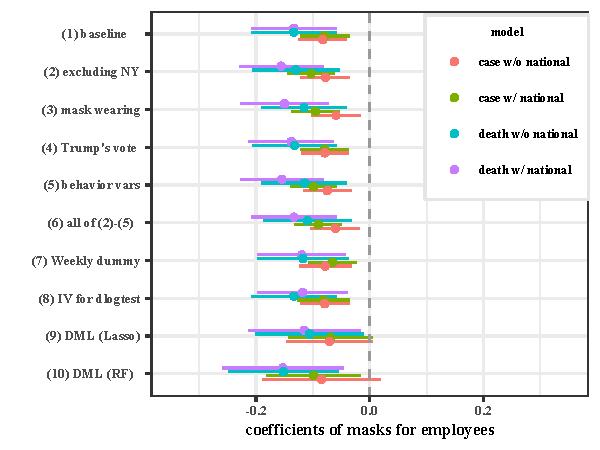
\includegraphics[width=0.5\textwidth]{tables_and_figures/pmaskbus-whisker-14}
      &
      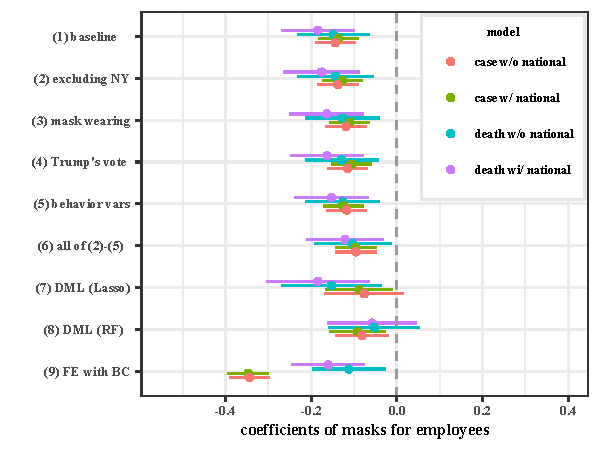
\includegraphics[width=0.5\textwidth]{tables_and_figures/pmaskbus-whisker-10} 
    \end{tabular}
  \end{minipage} \\\smallskip
    \begin{minipage}{\linewidth}
    \centering 
     {\textbf{(B)  closed K-12 Schools}}\\
    \medskip
    \begin{tabular}{cc}  
 $\quad$  (i) baseline timing$^\dagger$ &$\quad$ (ii) alternative timing$^\ddagger$\\ 
      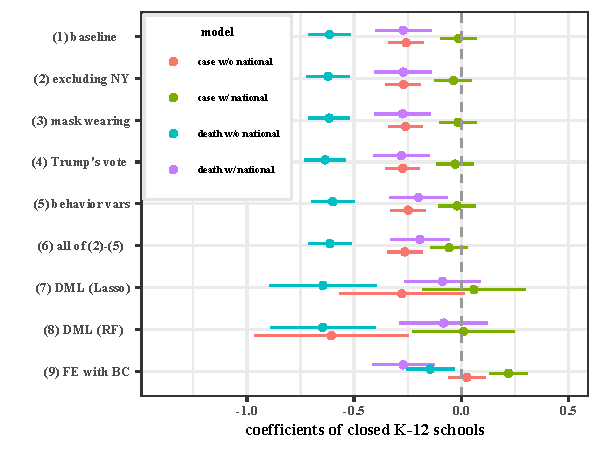
\includegraphics[width=0.5\textwidth]{tables_and_figures/pk12-whisker-14}
      &
      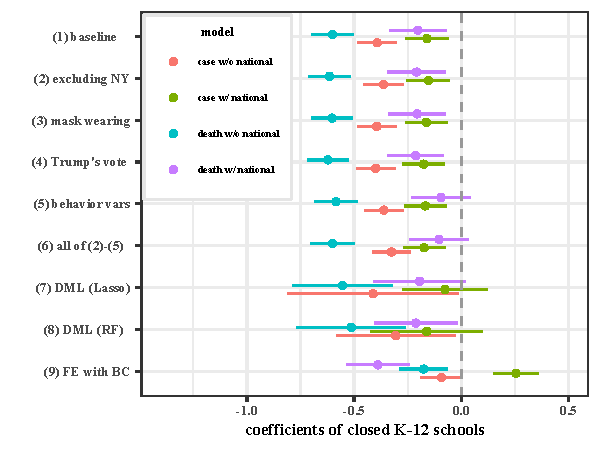
\includegraphics[width=0.5\textwidth]{tables_and_figures/pk12-whisker-10}
          \end{tabular}
  \end{minipage}  
    \begin{flushleft}
      \footnotesize
      $^\dagger$The times from exposure to case confirmation and death reporting  are assumed to be 14 and 21 days, respectively. $^\ddagger$The times from exposure to case confirmation and death reporting  are assumed to be 10 and 23 days, respectively. 
    \end{flushleft}
\end{figure}
   
   \addtocounter{figure}{-1}
\begin{figure}[ht]
  \caption{Estimated Coefficients for Policy Variables:  Sensitivity Analysis (cont.) \label{fig:whisker-2}}\bigskip
  \begin{minipage}{\linewidth}
    \centering
   {\textbf{(C)  stay-at-home orders}}\\
    \medskip
    \begin{tabular}{cc}  
 $\quad$  (i) baseline timing$^\dagger$ &$\quad$ (ii) alternative timing$^\ddagger$\\ 
      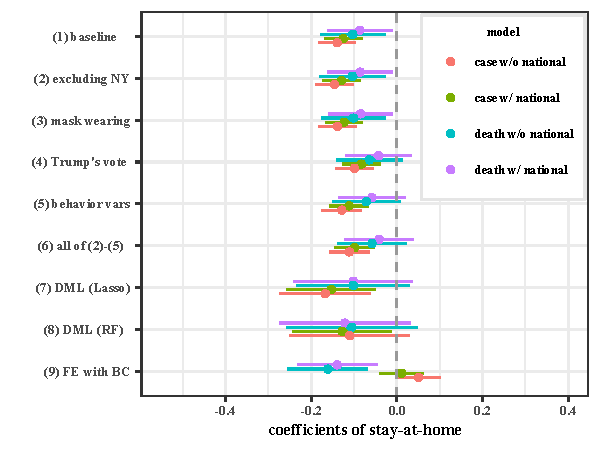
\includegraphics[width=0.5\textwidth]{tables_and_figures/pshelter-whisker-14}
      &
      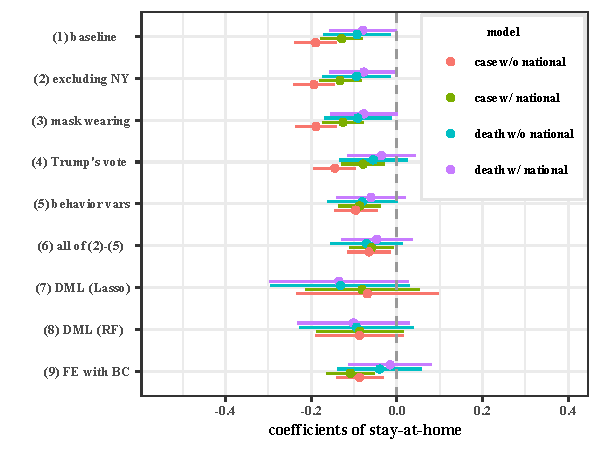
\includegraphics[width=0.5\textwidth]{tables_and_figures/pshelter-whisker-10} 
    \end{tabular}
  \end{minipage} \\ \smallskip
    \begin{minipage}{\linewidth}
    \centering 
     {\textbf{(D)  Average of stay-at-home, closed movie theaters, closed restaurants, and closed  businesses}}\\
    \medskip
    \begin{tabular}{cc}  
 $\quad$  (i) baseline timing$^\dagger$ &$\quad$ (ii) alternative timing$^\ddagger$\\ 
      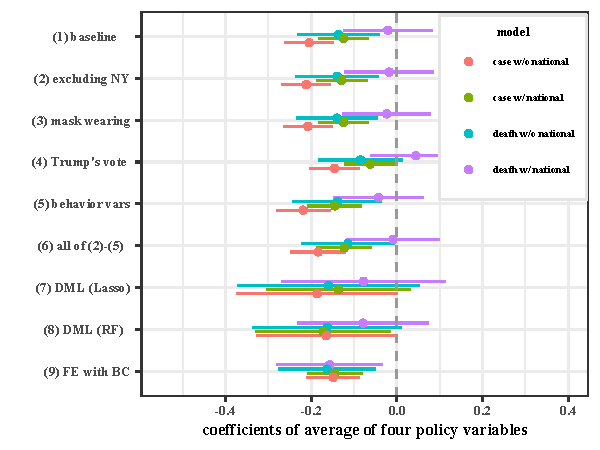
\includegraphics[width=0.5\textwidth]{tables_and_figures/pindex-whisker-14}
      &
      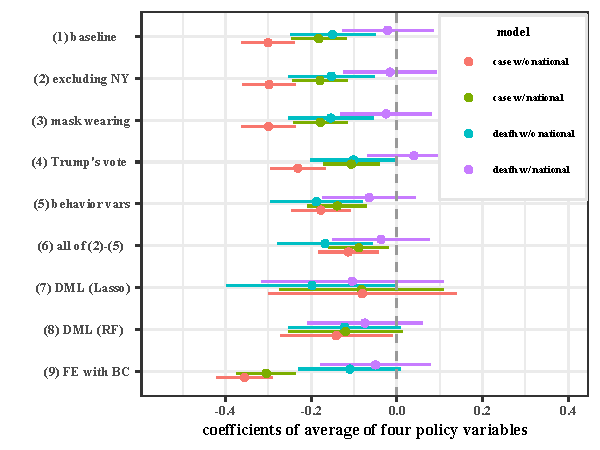
\includegraphics[width=0.5\textwidth]{tables_and_figures/pindex-whisker-10}
          \end{tabular}
  \end{minipage}   
    \begin{flushleft}
      \footnotesize
      $^\dagger$The times from exposure to case confirmation and death reporting  are assumed to be 14 and 21 days, respectively. $^\ddagger$The times from exposure to case confirmation and death reporting  are assumed to be 10 and 23 days, respectively. 
    \end{flushleft}
\end{figure}
   

 \begin{figure}
  \caption{Case and death growth conditional on school closures \label{fig:growthpolicies1}}
  \begin{minipage}{\linewidth}
    \centering
    \begin{tabular}{cc}
       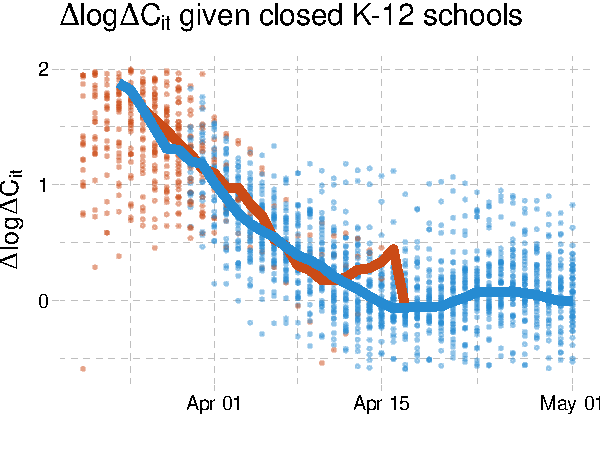
\includegraphics[width=0.483\textwidth]{tables_and_figures/pk12-cases-14}
      &
        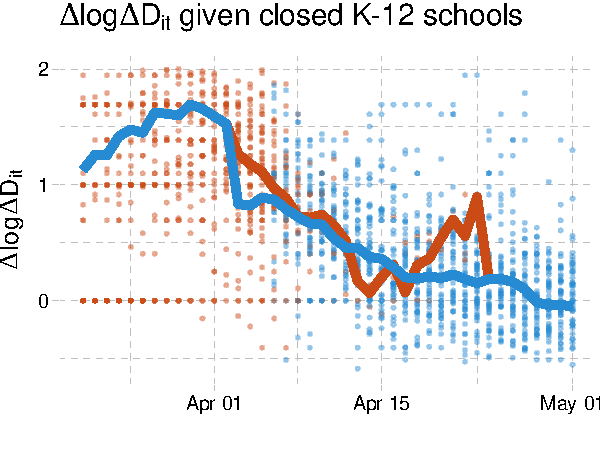
\includegraphics[width=0.483\textwidth]{tables_and_figures/pk12-deaths-21} 
    \end{tabular} 
      \footnotesize In these figures, red points are the case or death
      growth rate in states without each policy 14 (or 21 for deaths)
      days earlier. Blue points are states with each policy 14 (or 21
      for deaths) days earlier. The red line is the average across
      states without each policy. The blue line is the average across
      states with each policy.
  \end{minipage}
\end{figure}





    



\section{Empirical Evaluation of Counterfactual Policies}\label{counterfactuals}

We now turn our focus to dynamic feedback effects. Policy
and behavior changes that reduce case and death growth today can lead to a more
optimistic, riskier behavior in the future, attenuating longer run effects.
We perform the main counterfactual experiments using the average of two estimated coefficients as reported in column ``Average'' of Table \ref{tab:dieff-si} under a specification that excludes the number of past national cases and deaths from information variables. In the appendix, we also report additional counterfactual experiment results with the specification that includes the national information variables, and find that they are very similar. The results on mask policies, business closures, stay-at-home orders are robust with respect to this variation (see Figures \ref{fig:US-mask}-\ref{fig:US-shelter} in the appendix). On the other hand, the results on removing all policies, particularly closure of schools, reported in the next section, are sensitive to the inclusion of national information variables, highlighting the large uncertainty regarding the size of the effect.  In Figures \ref{fig:WA-mask}-\ref{fig:US-shelter} below, the top panel presents the result on cases while the bottom panel presents the result on deaths.

%Additional counterfactual experiments include the
%} %\footnote{\textbf{The results of counterfactual experiments are not sensitive to whether we use the estimate of  table \ref{tab:dieff-si} or that of table \ref{tab:dieff} except for a counterfactual experiment of removing all policies  in section \ref{removing-policies}.}}

\subsection{Business Mask Mandate}

\begin{figure}[ht]
  \caption{Effect of mandating masks on April 1st in Washington State \label{fig:WA-mask}}
  \begin{minipage}{\linewidth}
    \centering
    \begin{tabular}{ccc}
      \multicolumn{3}{c}{\textbf{Cases}} \\
      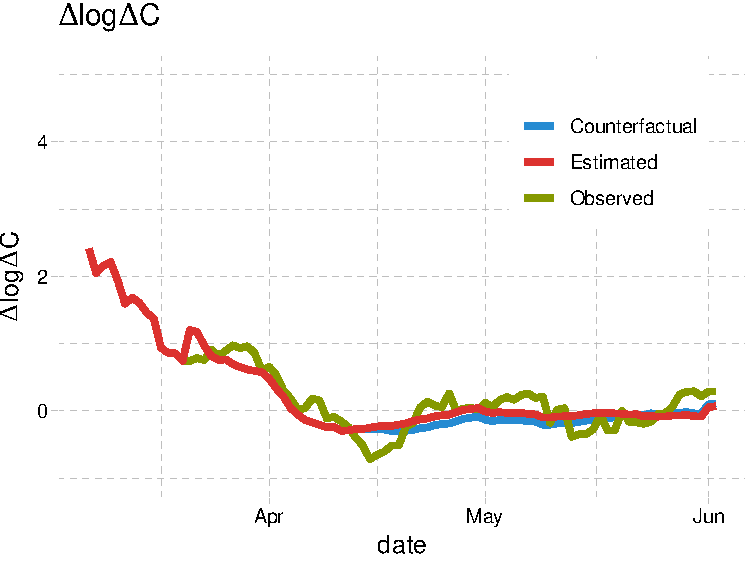
\includegraphics[width=0.31\textwidth]{tables_and_figures/Washington-mask-growth}
      &
        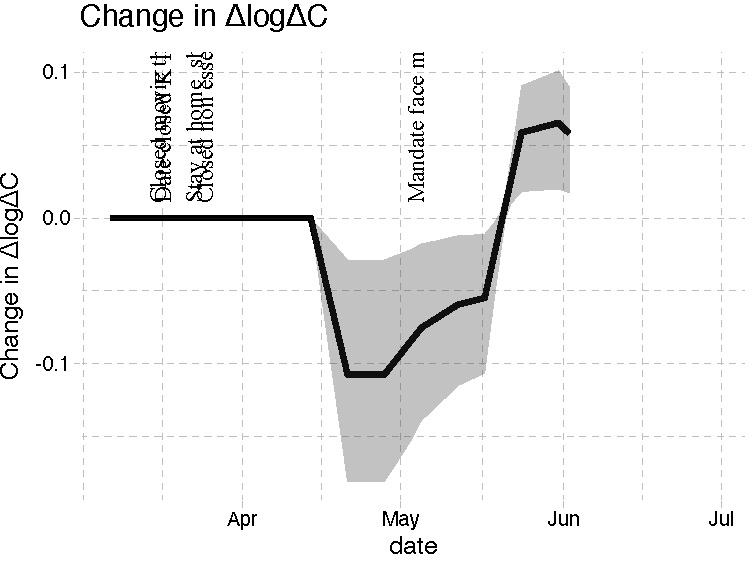
\includegraphics[width=0.31\textwidth]{tables_and_figures/Washington-mask-dgrowth_v1}
      &        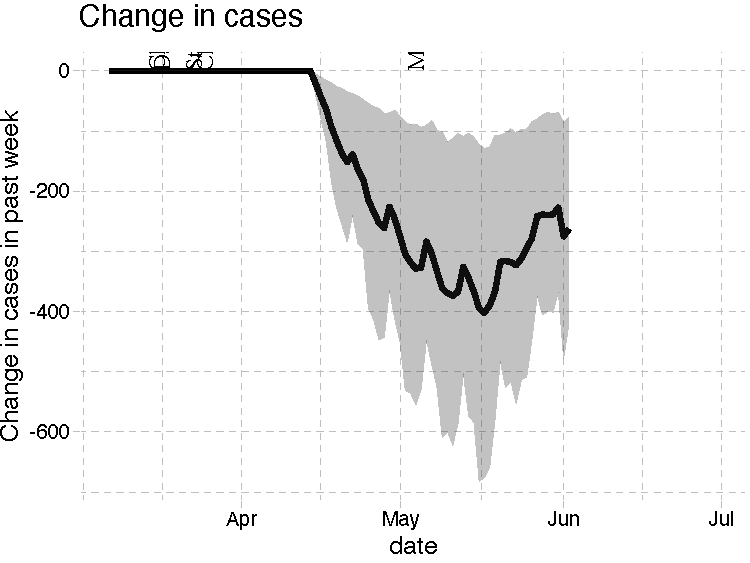
\includegraphics[width=0.31\textwidth]{tables_and_figures/Washington-mask-dcases_v1}
      \\
      \\
      \multicolumn{3}{c}{\textbf{Deaths}}
      \\      \includegraphics[width=0.31\textwidth]{tables_and_figures/Washington-mask-growth_deaths}
      &        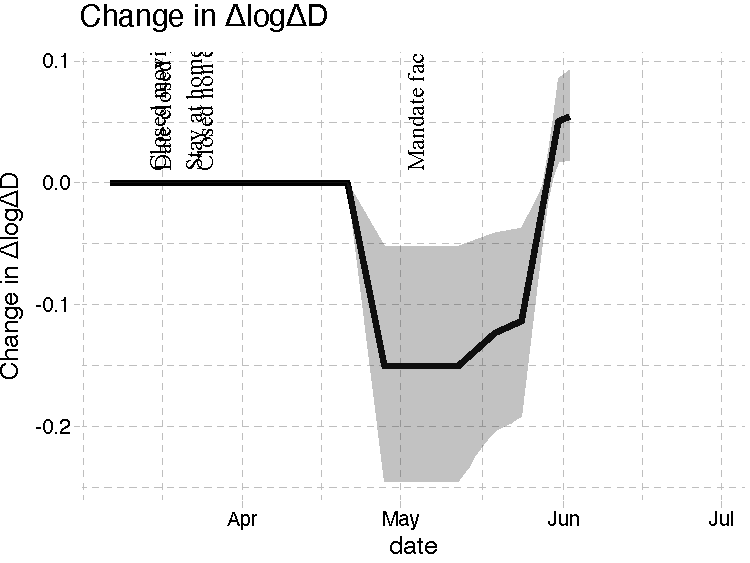
\includegraphics[width=0.31\textwidth]{tables_and_figures/Washington-mask-dgrowth_deaths_v1}
      &      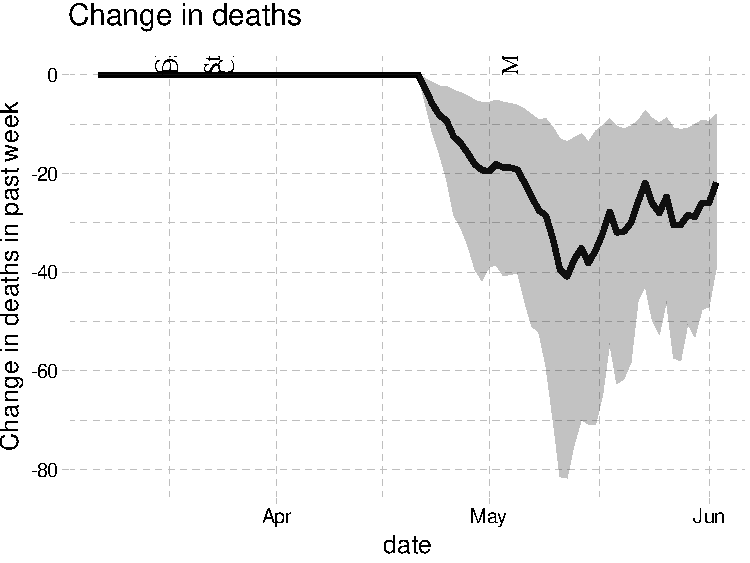
\includegraphics[width=0.31\textwidth]{tables_and_figures/Washington-mask-dcases_deaths_v1}
    \end{tabular}
    \begin{flushleft}
      \footnotesize To compute the estimated and counterfactual paths
      we use the average of two estimated coefficients as reported in
      column ``Average'' of Table \ref{tab:dieff-si}. We set initial
      $\Delta \log \Delta C$ and $\log \Delta C$ to their values first
      observed in the state we are simulating. We hold all other
      regressors at their observed values. Error terms are drawn with
      replacement from the residuals. We do this many times and report
      the average over draws of the residuals. The shaded region is a
      point-wise 90\% confidence interval.
    \end{flushleft}
  \end{minipage}
\end{figure}



We first consider the impact of a nationwide mask mandate for
employees beginning on April 1st. As discussed earlier, we find that
mask mandates reduce case and death growth even when holding behavior
constant. In other words, mask mandates may reduce infections with
relatively little economic disruption. This makes mask mandates a
particularly attractive policy instrument. In this section we examine
what would have happened to the number of cases if all states had imposed a mask
mandate on April 1st.\footnote{We feel this is a very plausible
  counterfactual policy. In a paper made publicly available on
  April 1st, \cite{abaluck2020} argued for mask usage based on
  comparisons between countries with and without pre-existing norms of
  widespread mask usage.}

For illustrative purpose, we begin by focusing on Washington State.
The
left column of  Figure \ref{fig:WA-mask} shows the observed, estimated
average, and counterfactual average of $\Delta \log \Delta C$ (top panel) and
$\Delta \log \Delta D$ (bottom panel). To compute the estimated and counterfactual
paths, we use the   estimate   in
column ``Average'' of Table \ref{tab:dieff-si}. We set initial
$\Delta \log \Delta C$ and $\log \Delta C$ to their values first
observed in the state we are simulating. We hold all other regressors
at their observed values. Error terms are drawn with replacement from
the residuals. We do this many times and report the average over draws
of the residuals. The shaded region is a point-wise 90\% confidence
interval. The left column shows that the fit of the estimated and
observed growth rate is quite good.

The middle column of Figure \ref{fig:WA-mask} shows the change in
growth rate from mandating masks on April 1st. The shaded region is a
90\% pointwise confidence interval. As shown, mandating masks on April
1st lowers the growth of cases or deaths 14 or 21 days later by 0.1 to
0.15. This effect then gradually declines due to information
feedback. Mandatory masks reduce past cases or deaths, which leads to
less cautious behavior, attenuating the impact of the policy. The
reversal of the decrease in growth in late April is due to our
comparison of a mask mandate on April 1st with Washington's actual
mask mandate in early May. By late April, the counterfactual mask
effect has decayed through information feedback, and we are comparing
it the undecayed impact of Washington's actual, later mask mandate.

The right column of Figure \ref{fig:WA-mask} shows how the changes in
case and death growth translate into changes in cases and deaths. The
estimates imply that mandating masks on April 1st would have led to
500 fewer cases and 250 fewer deaths in Washington by the start of
June.

\begin{figure}[ht]
  \caption{Effect of nationally mandating masks for employees on April
    1st in the US\label{fig:US-mask}}
  \begin{minipage}{\linewidth}
    \centering
    \medskip
    \begin{tabular}{cc}
      \multicolumn{2}{c}{\textbf{Cases}} \\
      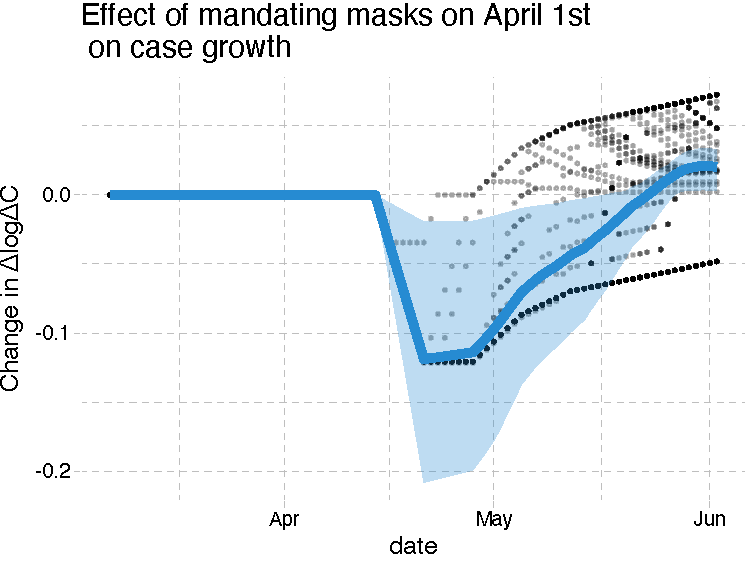
\includegraphics[width=0.49\textwidth]{tables_and_figures/us-mask-dgrowth_v1}
      &
        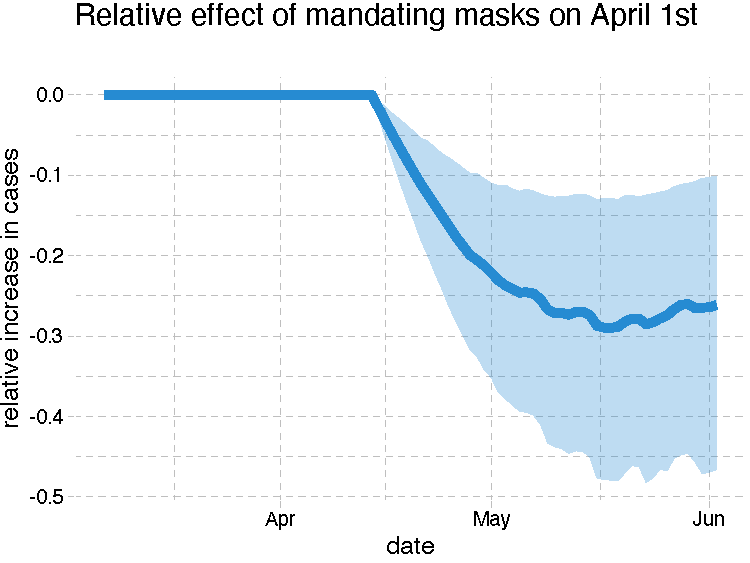
\includegraphics[width=0.49\textwidth]{tables_and_figures/us-mask-rel_v1}
      \\
      \\
      \multicolumn{2}{c}{\textbf{Deaths}} \\
      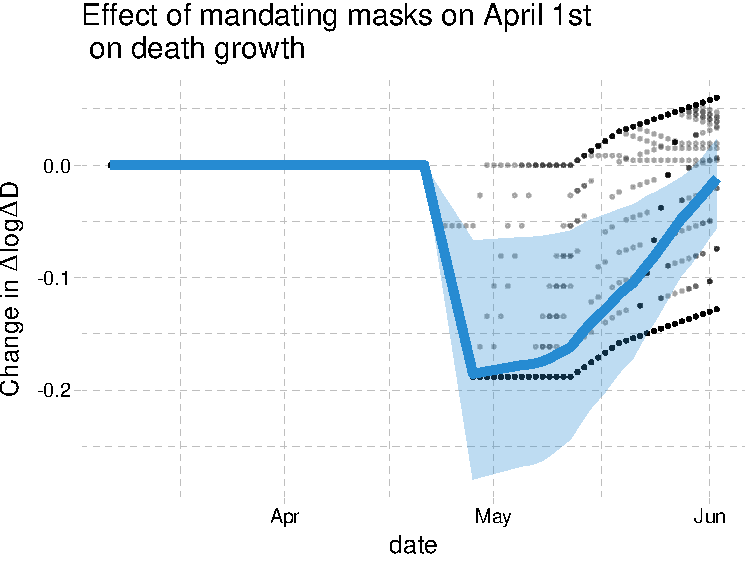
\includegraphics[width=0.49\textwidth]{tables_and_figures/us-mask-dgrowth_deaths_v1}
      &
        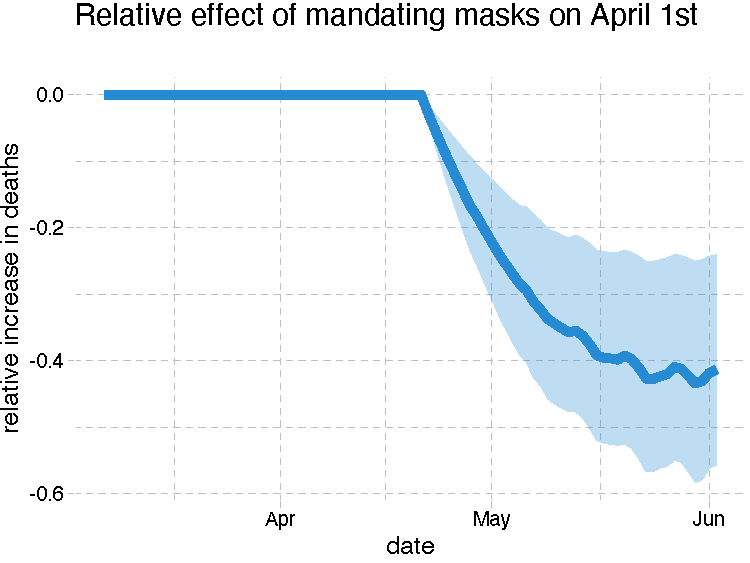
\includegraphics[width=0.49\textwidth]{tables_and_figures/us-mask-rel_deaths_v1}
    \end{tabular}
  \end{minipage}
    \begin{flushleft}
      \footnotesize In the left column, the dots are the average
      change in growth in each state. The blue line is the average
      across states of the change in growth. The shaded region is a
      point-wise 90\% confidence interval. The right column shows the
      change in cases or deaths relative to the baseline of actual
      policies.
    \end{flushleft}
\end{figure}


The results for other states are similar to those for Washington. In
the appendix, Figures  \ref{fig:MA-mask} and \ref{fig:IL-mask} display
similar results for Massachusetts and Illinois.
Figure \ref{fig:US-mask} shows the average change in cases and
deaths across states, where the top panel shows the effect on cases and the bottom panel shows the effect on deaths.
The point estimates indicate that mandating masks on April 1st
could have led to 25\% fewer cumulative cases and 37\% fewer
cumulative deaths by the end of May with their 90 percent intervals given by $[10,47]$\% and $[18,55]$\%, respectively. The result roughly translates into $18$ to $55$ thousand saved lives.

\subsection{Non-essential Business Closures}

A particularly controversial policy is the closure of non-essential
businesses. We now examine a counterfactual where non-essential
businesses are never closed. Figure \ref{fig:WA-nb} shows the effect
of leaving non-essential businesses open in Washington. The point
estimate implies that the closure of non-essential businesses reduced cases and
deaths by a small amount. However, this estimate is relatively
imprecise; 90\% confidence intervals for the change in cases and deaths from
leaving non-essential businesses open by the end of May are [-250,700] and
[-100,1200], respectively.

\begin{figure}[ht]
  \caption{Effect of leaving non-essential businesses open in Washington \label{fig:WA-nb}}
  \begin{minipage}{\linewidth}
    \centering
    \begin{tabular}{cc}
      \multicolumn{2}{c}{\textbf{Cases}} \\
      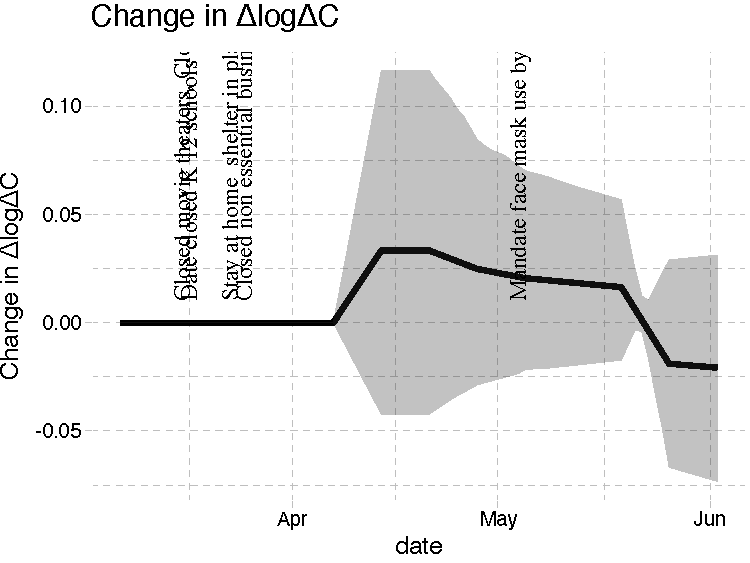
\includegraphics[width=0.45\textwidth]{tables_and_figures/Washington-nb-dgrowth_v1}
      &
        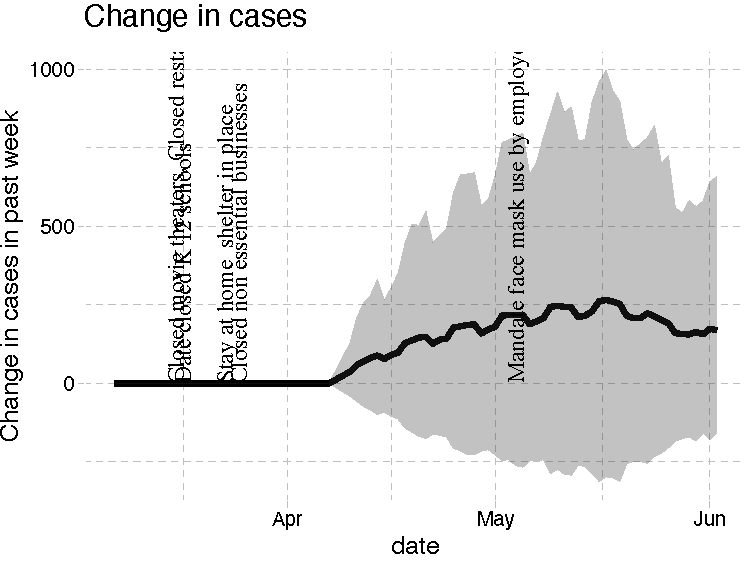
\includegraphics[width=0.45\textwidth]{tables_and_figures/Washington-nb-dcases_v1}\\
      \\
      \multicolumn{2}{c}{\textbf{Deaths}} \\
      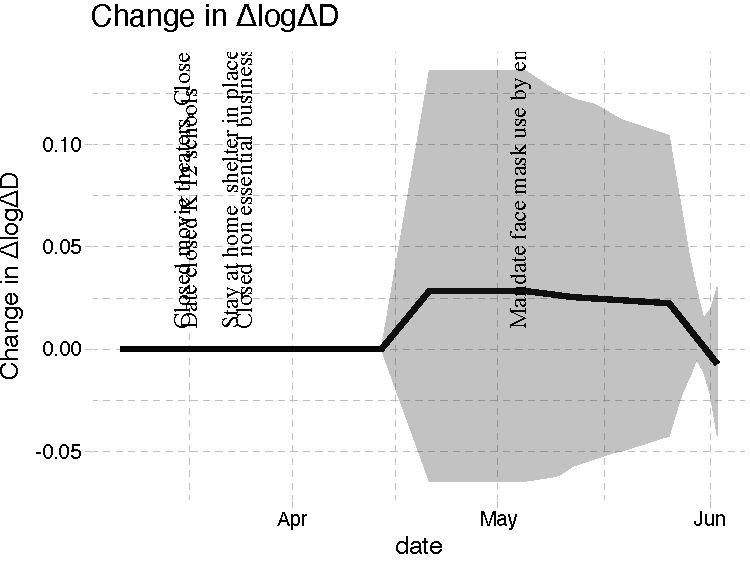
\includegraphics[width=0.45\textwidth]{tables_and_figures/Washington-nb-dgrowth_deaths_v1}
      & 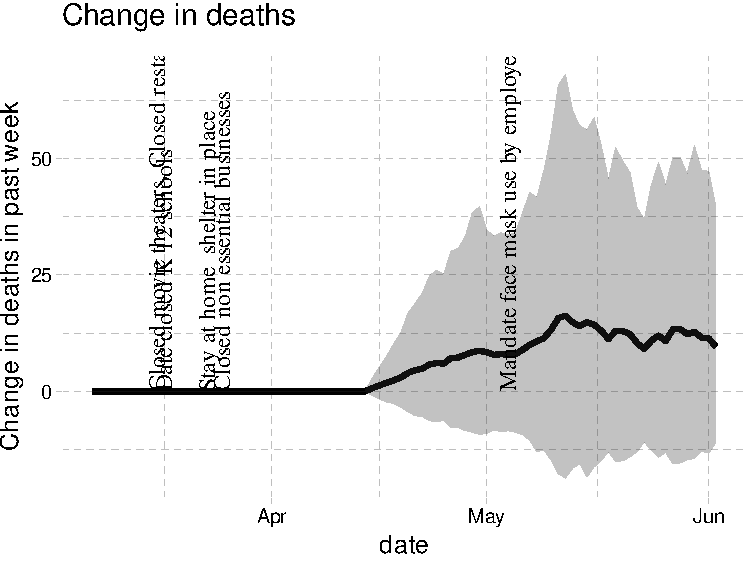
\includegraphics[width=0.45\textwidth]{tables_and_figures/Washington-nb-dcases_deaths_v1}
    \end{tabular}
  \end{minipage}
\end{figure}

Figure \ref{fig:US-nb} shows the national effect of leaving non
essential businesses open on cases and deaths. For cases, the
estimates imply that with non-essential businesses open, cases would
be about -15 to 60\% higher in late May. The results for deaths are
similar but less precise.

\begin{figure}[ht]
  \caption{Effect of leaving non-essential businesses open in the US\label{fig:US-nb}}
  \begin{minipage}{\linewidth}
    \centering
    \begin{tabular}{cc}
      \multicolumn{2}{c}{\textbf{Cases}} \\
      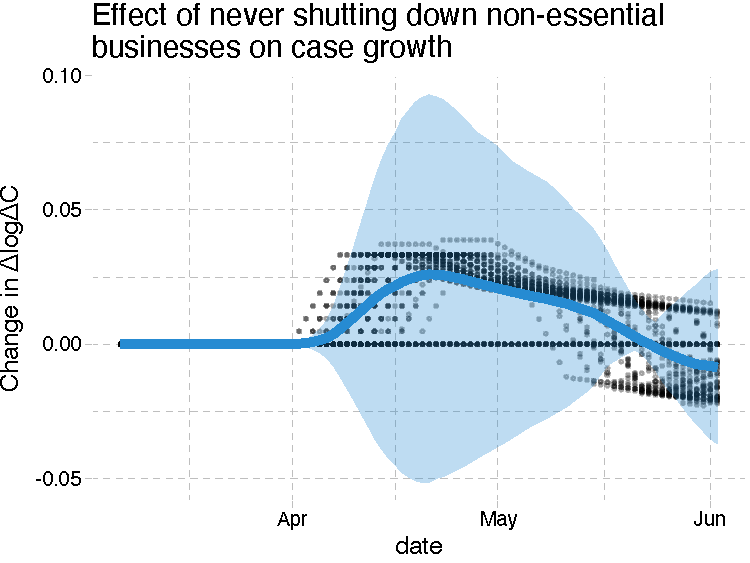
\includegraphics[width=0.45\textwidth]{tables_and_figures/us-nb-dgrowth_v1}
      &
        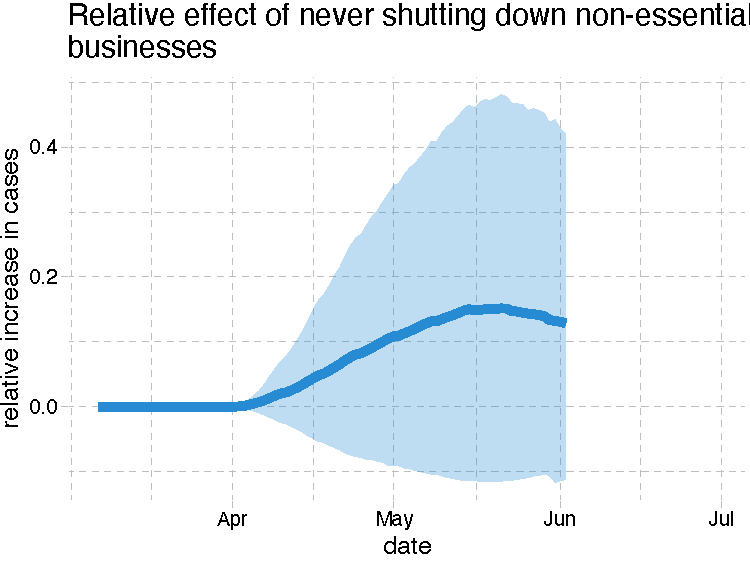
\includegraphics[width=0.45\textwidth]{tables_and_figures/us-nb-rel_v1}
      \\
      \\
      \multicolumn{2}{c}{\textbf{Deaths}} \\
      \includegraphics[width=0.45\textwidth]{tables_and_figures/us-nb-dgrowth_deaths_v1}
      &
        \includegraphics[width=0.45\textwidth]{tables_and_figures/us-nb-rel_deaths_v1}
    \end{tabular}
  \end{minipage}
\end{figure}

\subsection{Stay-at-home orders}

We next examine a counterfactual where stay-at-home orders had been never
issued.  Figure \ref{fig:US-shelter} shows the average effect of no
stay-at-home orders. On average, without stay-at-home orders, case
growth rate would have been nearly 0.1 higher in late April. This
translates to 80\% [25\%,170\%] more cases by the start of June. The
results for deaths are similar, but slightly less precise, with no
increase included in a 90 percent confidence interval.

\begin{figure}[ht]
  \caption{Effect of having no stay-at-home orders in the US\label{fig:US-shelter}}
  \begin{minipage}{\linewidth}
    \centering
    \begin{tabular}{cc}
      \multicolumn{2}{c}{\textbf{Cases}} \\
      \includegraphics[width=0.45\textwidth]{tables_and_figures/us-shelter-dgrowth_v1}
      &
        \includegraphics[width=0.45\textwidth]{tables_and_figures/us-shelter-rel_v1}
      \\
      \\
      \multicolumn{2}{c}{\textbf{Deaths}} \\
      \includegraphics[width=0.45\textwidth]{tables_and_figures/us-shelter-dgrowth_deaths_v1}
      &
        \includegraphics[width=0.45\textwidth]{tables_and_figures/us-shelter-rel_deaths_v1}
    \end{tabular}
  \end{minipage}
\end{figure}




\section{Counterfactual Effect of Removing All Policies and its Sensitivity}\label{removing-policies}




%We now consider the impact of changing from the observed policies to
%none.  Figure \ref{fig:WA-nb} shows the effect of removing all
%policies in Washington. The left column shows that without any policy
%intervention, case and death growth would have been higher by
%about 0.1 and 0.2. The confidence intervals are wide relative to the
%mean effect. In the right column, we see that the upper bounds of the
%confidence intervals include large increases in cases, and especially
%deaths.

%\begin{figure}[ht]
%  \caption{Effect of removing all policies in
%    Washington \label{fig:WA-nop}}
%  \begin{minipage}{\linewidth}
%    \centering
%    \begin{tabular}{cc}
%      \includegraphics[width=0.45\textwidth]{tables_and_figures/Washington-nop-dgrowth}
%      &
%        \includegraphics[width=0.45\textwidth]{tables_and_figures/Washington-nop-dcases}
%      \\
%      \includegraphics[width=0.45\textwidth]{tables_and_figures/Washington-nop-dgrowth_deaths}
%      &
%        \includegraphics[width=0.45\textwidth]{tables_and_figures/Washington-nop-dcases_deaths}
%    \end{tabular}
%  \end{minipage}
%\end{figure}

We now consider the impact of changing from the observed policies to none.
Figure \ref{fig:US-nop-SI} shows the average across states of the change
in case growth and relative increase in cases under a specification without past national case variables.
Removing policies leads to an increase of above 0.2 in
case growth throughout April and May. The confidence interval is
fairly wide, and its upper bound includes a very large increase in
cases by the end of May.  The right panel displays the national
increase in aggregate cases without any policy intervention. The
estimates imply at least a 7 fold increase in cases with a large upper bound by the end of May, or
at least 14 million additional cases. The estimated impact on deaths is larger than
cases, and even more imprecise.

The effect of removing all policies includes the effect of school
closures. The visual evidence on growth rates for states with and without school closures,
presented blow, suggest that there may be a potentially large effect, though the history is very short. The main results presented in Section 3 also support the hypothesis that the school closures were important at lowering the growth rates.  This evidence is consistent
with the emerging evidence of prevalence of Covid-19 among children
aged 10-17. \cite{children:nature} find that although children's
transmission and susceptibility rates are half that of ages 20-30,
children's contact rates are much higher.
This type of evidence, as well as, evidence that children carry viral
loads similar to older people (\cite{children:germany}), led Germany to make the early decision of closing schools.

\begin{figure}
  \caption{Case and death growth conditional on policies \label{fig:growthpolicies1}}
  \begin{minipage}{\linewidth}
    \centering
    \begin{tabular}{cc}
       \includegraphics[width=0.483\textwidth]{tables_and_figures/pk12-cases}
      &
        \includegraphics[width=0.483\textwidth]{tables_and_figures/pk12-deaths}
    \end{tabular}
    \footnotetext{ In these figures, red points are the case or death
      growth rate in states without each policy 14 (or 21 for deaths)
      days earlier. Blue points are states with each policy 14 (or 21
      for deaths) days earlier. The red line is the average across
      states without each policy. The blue line is the average across
      states with each policy.}
  \end{minipage}
\end{figure}


As discussed above, there is little variation across states
in the timing of school closures. Consequently, the effect of school
closures is difficult to identify statistically, because it is hard to separate it from aggregate time effect, and its estimate is sensitive to an inclusion of some aggregate variables such as national cases. To support this point, Figure \ref{fig:US-nop} shows the
effect of removing all policies on cases based on the estimates with national cases
included as information. When national case variables are included
in the specification, the estimated effect of school closures, and hence that of removing all
policies, is much smaller with a 90\% confidence interval of [0,10] fold increases.

Given this sensitivity, we conclude that there still exists a lot of uncertainty as to the effect of removing all policies, especially schooling. The impact of not implementing any policies on cases and deaths can be quite large, but  the effect of school closures, hence that of removing all policies, is not well identified statistically from the US state-level data alone, because of the lack of cross-sectional variations.  Any analyses of re-opening plans need to be aware of this uncertainty.  An important research question is how to resolve this uncertainty using additional data sources.

\begin{figure}[ht]
  \caption{Effect of removing policies on cases in the US under a specification with only state-level cases/deaths as information \label{fig:US-nop-SI}}
  \begin{minipage}{\linewidth}
    \centering
    \begin{tabular}{cc}
      \includegraphics[width=0.45\textwidth]{tables_and_figures/us-nop-dgrowth_v1}
      &
        \includegraphics[width=0.45\textwidth]{tables_and_figures/us-nop-rel_v1}
%      \\
%      \includegraphics[width=0.45\textwidth]{tables_and_figures/us-nop-dgrowth_deaths_v1}
%      &
%        \includegraphics[width=0.45\textwidth]{tables_and_figures/us-nop-rel_deaths_v1}
    \end{tabular}
  \end{minipage}
\end{figure}

\begin{figure}[ht]
  \caption{Effect of removing policies on cases in the US under a specification with both
  state-level cases/deaths and national-level cases/deaths as information \label{fig:US-nop}}
  \begin{minipage}{\linewidth}
    \centering
    \begin{tabular}{cc}
      \includegraphics[width=0.45\textwidth]{tables_and_figures/us-nop-dgrowth}
      &
        \includegraphics[width=0.45\textwidth]{tables_and_figures/us-nop-rel}
%      \\
%      \includegraphics[width=0.45\textwidth]{tables_and_figures/us-nop-dgrowth_deaths}
%      &
%        \includegraphics[width=0.45\textwidth]{tables_and_figures/us-nop-rel_deaths}
    \end{tabular}
  \end{minipage}
\end{figure}





%%%%%%%%%%%%%%%%%%%%%%%%%%%%%%%%%%%%%%%%%%%%%%%%%%%%%%%%%%%%%%%%%%%%%%%%%%%%%%%%

\afterpage{\clearpage}

\section{Conclusion}


This paper assesses the effects of policies on the spread of Covid-19 in the US using state-level data on cases, tests, policies, and social distancing behavior measures from Google Mobility Reports. Our findings are summarized as follows.

First, our empirical analysis indicates that mandating face masks has reduced the spread of Covid-19 without affecting people's social distancing behavior measured by Google Mobility Reports. Our counterfactual experiment based on the estimated model suggests that if all states had have adopted mandatory face mask policies on April 1st of 2020, then the number of deaths by the end of May would have been smaller by as much as  $17$ to $55$\%, which roughly translates to $17$ to $55$ thousand saved lives.

Second, we find that keeping non-essential businesses open would have led to -20 to 60\% more cases  while not implementing stay-at-home orders would have increased cases by 25 to 170 \% by the start of June. % Except for mask mandates, the effect of all other policies on case and death growth is realized through their impact on social distancing behavior.

Third, we find considerable uncertainty over  the impact of all policies combined on case or death growth because it is difficult to identify the effect of school closures from the US state-level data due to the lack of variation in the timing of school closures across states.

Fourth, our analysis shows that people voluntarily reduce their visits to workplace, retails, grocery stores, and limit their use of public transit when they receive  information on a higher number of new cases and deaths. This suggests that individuals make decisions to voluntarily limit their contact with others in response to greater transmission risks, leading to an important feedback mechanism that affects future cases and deaths. Model simulations that ignore this voluntary behavioral response to information on transmission risks would over-predict the future number of cases and deaths.

Beyond these findings, our paper presents a useful conceptual framework to investigate the relative roles of policies and information on determining the spread of Covid-19 through their impact on people's behavior. Our causal model allows us  to explicitly define counterfactual scenarios to properly evaluate the effect of alternative policies on the spread of Covid-19. %, and can be used to quantitatively examine various Covid-19 related issues  for future research.
 More broadly, our  causal framework can be useful for quantitatively analyzing not only health outcomes but also various economic outcomes \citep{bartik2020, chetty2020real}.





\FloatBarrier

\begin{footnotesize}

\bibliographystyle{jpe}
\bibliography{covid}

\end{footnotesize}


\newpage

\appendix

\section{Data Construction}


\subsection{Measuring $\Delta C$ and $\Delta\log \Delta C$}

We have three data sets with information on daily cumulative confirmed
cases in each state. As shown in Table \ref{tab:casecor}, these
cumulative case numbers are very highly correlated. However, Table
\ref{tab:casediff} shows that the numbers are different more often
than not.

% latex table generated in R 4.0.2 by xtable 1.8-4 package
% Fri Aug 14 16:39:05 2020
\begin{table}[ht]
\centering
\begin{tabular}{rrrr}
  \hline
 & NYT & JHU & CTP \\ 
  \hline
NYT & 1.00000 & 0.99985 & 0.99970 \\ 
  JHU & 0.99985 & 1.00000 & 0.99985 \\ 
  CTP & 0.99970 & 0.99985 & 1.00000 \\ 
   \hline
\end{tabular}
\caption{Correlation of cumulative cases \label{tab:casecor}} 
\end{table}


% latex table generated in R 4.0.2 by xtable 1.8-4 package
% Tue Aug 11 13:30:13 2020
\begin{table}[ht]
\centering
\begin{tabular}{rrrr}
  \hline
 & 1 & 2 & 3 \\ 
  \hline
NYT & 1.00 & 0.23 & 0.31 \\ 
  JHU & 0.23 & 1.00 & 0.30 \\ 
  CTP & 0.31 & 0.30 & 1.00 \\ 
   \hline
\end{tabular}
\caption{Portion of cumulative cases that are equal between data sets\label{tab:casediff}} 
\end{table}


Figure \ref{fig:dailycases} shows the evolution of new cases in each
of these three datasets. In all cases, daily changes in cumulative
cases displays some excessive volatility. This is likely due to delays
and bunching in testing and reporting of results. Table
\ref{tab:newcasecor} shows the variance of log new cases in each data
set, as well as their correlations. As shown, the correlations are
approximately $0.9$. The NYT new case
numbers have the lowest variance.\footnote{This comparison is somewhat
  sensitive to how you handle negative and zero cases when taking
  logs. Here, we replaced $\log(0)$ with $-1$. In our main
  results, we work with weekly new cases, which are very rarely zero.}
In our subsequent results, we will primarily use the case numbers from
The New York Times.

\begin{figure}[!ht]\caption{Daily cases \label{fig:dailycases}}
  \centering
  \begin{minipage}{\textwidth}
    \centering
    \includegraphics[width=0.45\textwidth]{tables_and_figures/newcases}
    \footnotetext{Each line shows daily new cases in a state.}
  \end{minipage}
\end{figure}

% latex table generated in R 4.0.0 by xtable 1.8-4 package
% Mon Aug 10 20:07:02 2020
\begin{table}[ht]
\centering
\begin{tabular}{rrrr}
  \hline
 & NYT & JHU & CTP \\ 
  \hline
NYT & 1.00 & 0.89 & 0.85 \\ 
  JHU & 0.89 & 1.00 & 0.79 \\ 
  CTP & 0.85 & 0.79 & 1.00 \\ 
  Variance & 5.23 & 6.57 & 6.28 \\ 
   \hline
\end{tabular}
\caption{Correlation and variance of log daily new cases\label{tab:newcasecor}} 
\end{table}


For most of our results, we focus on new cases in a week instead of in
a day. We do this for two reasons as discussed in the main text. First, a decline of new cases over
two weeks has become a key metric for decision makers. Secondly, aggregating to weekly new cases smooths out the noise associated with  the timing of
reporting and testing.

Table \ref{tab:weekcasecor} reports the correlation and variance of
weekly log new cases across the three data sets. Figure
\ref{fig:weekcases} shows the evolution of weekly new cases in each
state over time.

% latex table generated in R 4.0.0 by xtable 1.8-4 package
% Wed Jul 29 09:27:21 2020
\begin{table}[ht]
\centering
\begin{tabular}{rrrr}
  \hline
 & NYT & JHU & CTP \\ 
  \hline
NYT & 1.00 & 0.98 & 0.98 \\ 
  JHU & 0.98 & 1.00 & 0.97 \\ 
  CTP & 0.98 & 0.97 & 1.00 \\ 
  Variance & 3.79 & 3.99 & 3.55 \\ 
   \hline
\end{tabular}
\caption{Correlation and variance of log weekly new cases\label{tab:weekcasecor}} 
\end{table}


\begin{figure}[!ht]\caption{Weekly Cases \label{fig:weekcases}}
  \centering
  \begin{minipage}{\textwidth}
    \centering
    \includegraphics[width=0.45\textwidth]{tables_and_figures/weekcases}
    \footnotetext{Each line shows weekly new cases in a state.}
  \end{minipage}
\end{figure}

\subsection{Deaths}

Table \ref{tab:weekdeathcor} reports the correlation and variance of
weekly deaths in the three data sets. Figure \ref{fig:weekdeaths}
shows the evolution of weekly deaths in each state. As with cases, we
use death data from The New York Times in our main results.

% latex table generated in R 4.0.0 by xtable 1.8-4 package
% Fri Jul 31 09:17:29 2020
\begin{table}[ht]
\centering
\begin{tabular}{rrrr}
  \hline
 & NYT & JHU & CTP \\ 
  \hline
NYT & 1.00 & 0.99 & 0.99 \\ 
  JHU & 0.99 & 1.00 & 0.98 \\ 
  CTP & 0.99 & 0.98 & 1.00 \\ 
  Variance & 183940.46 & 188236.24 & 130900.77 \\ 
   \hline
\end{tabular}
\caption{Correlation and variance of weekly deaths\label{tab:weekdeathcor}} 
\end{table}


\begin{figure}[!ht]\caption{Weekly Deaths \label{fig:weekdeaths}}
  \centering
  \begin{minipage}{\textwidth}
    \centering
    \includegraphics[width=0.45\textwidth]{tables_and_figures/weekdeaths}
    \footnotetext{Each line shows weekly deaths in a state.}
  \end{minipage}
\end{figure}


\begin{figure}[!ht]\caption{Case and death growth \label{fig:growthq}}
  \centering
  \begin{minipage}{\textwidth}
    \centering
    \begin{tabular}{c}
      \includegraphics[width=0.75\textwidth]{tables_and_figures/casequantiles}
      \\
      \includegraphics[width=0.75\textwidth]{tables_and_figures/deathquantiles}
      \footnotetext{Thin gray lines are case or death growth in each
      state and date. Thicker colored lines are quantiles of case or
      death growth conditional on date.}
    \end{tabular}
  \end{minipage}
\end{figure}


\subsection{Tests}

Our test data comes from The Covid Tracking Project. Figure
\ref{fig:test} shows the evolution of tests over time.

\begin{figure}[!ht]\caption{Number of Tests \label{fig:test}}
  \centering
  \begin{minipage}{\textwidth}
    \centering
    \includegraphics[width=0.45\textwidth]{tables_and_figures/test}
    \footnotetext{These figures use the ``total test results''
      reported by The Covid Tracking Project. This is meant to reflect
      the number of people tested
      (\href{https://covidtracking.com/about-data/faq}{as opposed to
        the number of specimens tested}).}
  \end{minipage}
\end{figure}

\FloatBarrier

\subsection{Social Distancing Measures}

In measuring social distancing, we focus on Google Mobility
Reports. This data has international coverage and is publicly
available. Figure \ref{fig:gmr} shows the evolution of the four Google
Mobility Reports variables that we use in our analysis.

%% The following is true but we haven't included any of the
%% results. We can add if needed.
% We also compare Google Mobility Reports to other social
% distancing measures from SafeGraph, Unacast, and PlaceIQ. Each of
% these other data sources are limited to the United States. SafeGraph
% and Unacast data is not publicly available (both companies make the
% data available to researchers at no cost).
\begin{figure}[ht]\caption{Evolution of Google Mobility Reports \label{fig:gmr}}
  \begin{minipage}{\linewidth}
    \begin{tabular}{cc}
      \includegraphics[width=0.5\linewidth]{tables_and_figures/workplaces}
      &
      \includegraphics[width=0.5\linewidth]{tables_and_figures/retail}
      \\
      \includegraphics[width=0.5\linewidth]{tables_and_figures/grocery}
      &
      \includegraphics[width=0.5\linewidth]{tables_and_figures/transit}
    \end{tabular}
    \footnotetext{This figure shows the evolution of Google Mobility
      Reports over time. Thin gray lines are the value of the
      variables in each state and date. Thicker colored lines are
      quantiles of the variables conditional on date.}
  \end{minipage}
\end{figure}


\subsection{Policy Variables}

We use the database on US state policies created by
\cite{raifman2020}. %This database records that each state implemented 25 Covid-19 related policies.
As discussed in the main text, our analysis focuses on seven policies. For stay-at-home orders, closed nonessential
businesses, closed K-12 schools, closed restaurants except takeout,
and closed movie theaters, we double-checked any
state for which \cite{raifman2020} does not record a date. We filled
in a few missing dates. Our modified data is available
\href{"https://docs.google.com/spreadsheets/d/1E6HRkgbdSnZ9ZxrneydU6q4hhOCCt9oTl_5fa3OFVZE/edit?usp=sharing}{here}. Our
modifications fill in 1 value for school closures, 2 for stay-at-home orders, 3 for movie theater closure, and 4 for
non-essential business closures. Table \ref{tab:policies} displays all 25 dated policy variables in
\cite{raifman2020}'s database with our modifications described above.


\afterpage{%
  \clearpage% Flush earlier floats (otherwise order might not be correct)
  \thispagestyle{empty}% empty page style (?)
  \begin{landscape}% Landscape page
    \centering % Center table
    % latex table generated in R 4.0.2 by xtable 1.8-4 package
% Thu Aug 27 21:46:23 2020
\begin{table}[ht]
\centering
\begin{tabular}{rllll}
  \hline
 & N & Min & Median & Max \\ 
  \hline
State of emergency & 51 & 2020-02-29 & 2020-03-11 & 2020-03-16 \\ 
  Date closed K 12 schools & 51 & 2020-03-13 & 2020-03-17 & 2020-04-03 \\ 
  Closed day cares & 15 & 2020-03-16 & 2020-03-23 & 2020-04-06 \\ 
  Date banned visitors to nursing homes & 30 & 2020-03-09 & 2020-03-16 & 2020-04-06 \\ 
  Closed non essential businesses & 43 & 2020-03-19 & 2020-03-25 & 2020-04-06 \\ 
  Closed restaurants except take out & 48 & 2020-03-15 & 2020-03-17 & 2020-04-03 \\ 
  Closed gyms & 49 & 2020-03-16 & 2020-03-20 & 2020-04-03 \\ 
  Closed movie theaters & 49 & 2020-03-16 & 2020-03-21 & 2020-04-06 \\ 
  Stay at home  shelter in place & 42 & 2020-03-19 & 2020-03-28 & 2020-04-07 \\ 
  End relax stay at home shelter in place & 39 & 2020-04-24 & 2020-05-18 & 2020-06-19 \\ 
  Began to reopen businesses statewide & 50 & 2020-04-20 & 2020-05-07 & 2020-06-05 \\ 
  Reopen restaurants & 48 & 2020-04-24 & 2020-05-18 & 2020-06-22 \\ 
  Reopened gyms & 44 & 2020-04-24 & 2020-05-18 & 2020-07-13 \\ 
  Reopened movie theaters & 37 & 2020-04-27 & 2020-06-01 & 2020-07-13 \\ 
  Resumed elective medical procedures & 35 & 2020-04-20 & 2020-04-30 & 2020-05-29 \\ 
  Mandate face mask use by all individuals in public spaces & 35 & 2020-04-08 & 2020-06-26 & 2020-08-05 \\ 
  Mandate face mask use by employees in public facing businesses & 44 & 2020-04-03 & 2020-05-01 & 2020-08-03 \\ 
  Stop Initiation of Evictions overall or due to COVID related issues & 30 & 2020-03-16 & 2020-03-24 & 2020-05-30 \\ 
  Stop enforcement of evictions overall or due to COVID related issues & 29 & 2020-03-15 & 2020-03-24 & 2020-06-08 \\ 
  Renter grace period or use of security deposit to pay rent & 3 & 2020-04-10 & 2020-04-24 & 2020-05-20 \\ 
  Order freezing utility shut offs & 34 & 2020-03-12 & 2020-03-19 & 2020-04-13 \\ 
  Froze mortgage payments & 1 & 2020-03-21 & 2020-03-21 & 2020-03-21 \\ 
  Waived one week waiting period for unemployment insurance & 36 & 2020-03-08 & 2020-03-18 & 2020-04-06 \\ 
   \hline
\end{tabular}
\caption{State Policies \label{tab:policies}} 
\end{table}

  \end{landscape}
  \clearpage% Flush page
}

\begin{figure}
  \caption{Case and death growth conditional on policies \label{fig:growthpolicies1}}
  \begin{minipage}{\linewidth}
    \centering
    \begin{tabular}{cc}
      \includegraphics[width=0.483\textwidth]{tables_and_figures/pmaskbus-cases-14}
      &
        \includegraphics[width=0.483\textwidth]{tables_and_figures/pmaskbus-deaths-21}
      \\
      \includegraphics[width=0.483\textwidth]{tables_and_figures/pk12-cases-14}
      &
        \includegraphics[width=0.483\textwidth]{tables_and_figures/pk12-deaths-21}
      \\
      \includegraphics[width=0.483\textwidth]{tables_and_figures/pshelter-cases-14}
      &
        \includegraphics[width=0.483\textwidth]{tables_and_figures/pshelter-deaths-21}
      \\
    \end{tabular}
    \footnotetext{ In these figures, red points are the case or death
      growth rate in states without each policy 14 (or 21 for deaths)
      days earlier. Blue points are states with each policy 14 (or 21
      for deaths) days earlier. The red line is the average across
      states without each policy. The blue line is the average across
      states with each policy.}
  \end{minipage}
\end{figure}

\begin{figure}
  \caption{Case and death growth conditional on policies \label{fig:growthpolicies2}}
  \begin{minipage}{\linewidth}
    \centering
    \begin{tabular}{cc}
      \includegraphics[width=0.483\textwidth]{tables_and_figures/pmovie-cases-14}
      &
        \includegraphics[width=0.483\textwidth]{tables_and_figures/pmovie-deaths-21}
      \\
      \includegraphics[width=0.483\textwidth]{tables_and_figures/prestaurant-cases-14}
      &
        \includegraphics[width=0.483\textwidth]{tables_and_figures/prestaurant-deaths-21}
      \\
      \includegraphics[width=0.483\textwidth]{tables_and_figures/pnonessential-cases-14}
      &
        \includegraphics[width=0.483\textwidth]{tables_and_figures/pnonessential-deaths-21}
    \end{tabular}
    \footnotetext{ In these figures, red points are the case or death
      growth rate in states without each policy 14 (or 21 for deaths)
      days earlier.  Blue points are states with each policy14 (or 21
      for deaths) days earlier.  The red line is the average across
      states without each policy. The blue line is the average across
      states with each policy.}
  \end{minipage}
\end{figure}

\subsection{Timing\label{sec:timing}}

There is a delay between infection and when a person is tested and
appears in our case data. \cite{midas2020} maintain a list of
estimates of the duration of various stages of Covid-19
infections. The incubation period, the time from infection to symptom
onset, is widely believed to be 5 days. For example, using data from
Wuhan, \cite{li2020} estimate a mean incubation period of 5.2 days.
\cite{siorda2020} reviews the literature and concludes the mean
incubation period is 3-9 days.

Estimates of the time between symptom onset and case reporting or death
are less common. Using Italian data, \cite{cereda2020} estimate an
average of 7.3 days between symptom onset and
reporting. \cite{zhang2020} find an average of 7.4 days using Chinese data
from December to early February, but they find this period declined
from 8.9 days in January to 5.4 days in the first week of
February. Both of these papers on time from symptom onset to reporting
have large confidence intervals covering approximately 1 to 20 days.

Studying publicly available data on infected persons diagnosed outside of Wuhan,
\cite{linton2020}  estimate an average of 15 days  from  onset to death. Similarly, using publicly available reports of 140 confirmed Covid-19 cases in China, mostly outside Hubei Province, \cite{sanche2020} estimate the time from onset to death to be  16.1 days.

Based on the above, we expect a delay of roughly two weeks between
changes in behavior or policies, and changes in reported
cases while a corresponding delay of roughly three weeks for deaths.

% Our growth rate variable,
% $$
% {\ycolor Y_{it}} = \Delta \log \Delta C_{t} = \log(C_{t} - C_{t-7}) - \log(C_{t-7}-C_{t-14})
% $$
% reflects an average growth rate of cases from time $t-7$ to $t$.\footnote{This
% can be seen applying the intermediate value theorem to the dynamics
% of the SIR model from section \label{sec:sirmodel}. Specifically,
% \begin{align*}
%   C_{t} - C_{t-7} = & \int_{t-7}^t \dot{C}(s) ds \\
%   = & \int_{t-7}^t \tau(s) I(s) ds \\
%   = & \overline{\tau}(t-7,t) I(t-7) \int_{t-7}^t \exp(\int_{t-7}^s \frac{S(r)}{N}
%       \beta(r) - \gamma(r) dr \right) ds \\
%   = & \overline{\tau}(t-7,t) \overline{\exp(\frac{S}{N} \beta - \gamma)}(t-7,t) I(t-7) \\
%   = & \overline{\tau}(t-7,t) \overline{\exp(\frac{S}{N} \beta -
%       \gamma)}(t-7,t)
%       \overline{\exp(\frac{S}{N} \beta - \gamma)}(t-14,t-7) I(t-14)
% \end{align*}
% where $\gamma(r) = \frac{S(r-\ell)}{N}\beta(r-\ell)$ and expressions
% with a line over them are constants that exist by the intermediate
% value theorem. $\overline{\exp(\frac{S}{N} \beta - \gamma)}(t-7,t)$ is
% a constant growth rate from $t-7$ to $t$ that gives rise to the same
% number of infections at time $t$ as the original, potentially time
% varying, growth rate. Applying similar reasoning to
% $C_{t-7} - C_{t-14}$ and combining gives
% \begin{align*}
%   {\ycolor Y_{it}} = \log(C_{t} - C_{t-7}) - \log(C_{t-7}-C_{t-14})
%   = & \overline{\exp(\frac{S}{N} \beta -  \gamma)}(t-7,t) +
%       \log(\overline{\tau}(t-7,t)) -  \log(\overline{\tau}(t-14,t-7)).
% \end{align*}
% }

\FloatBarrier


\end{document}



\subsection{Counterfactuals for Massachusetts and
  Illinois}
 Figures \ref{fig:MA-mask} and \ref{fig:IL-mask} present the fit of estimated cases as well as the counterfactual effect of mandating masks on April 1st in Massachusetts and Illinois, respectively. Figures \ref{fig:MA-nb} and \ref{fig:IL-nb}   show the counterfactual effect of leaving non-essential business open in Massachusetts and Illinois, respectively.

\FloatBarrier

\begin{figure}[b]
  \caption{Effect of mandating masks on April 1st in Massachusetts \label{fig:MA-mask}}
  \begin{minipage}{\linewidth}
    \centering
    \begin{tabular}{ccc}
      \multicolumn{3}{c}{\textbf{Cases}} \\
      \includegraphics[width=0.31\textwidth]{tables_and_figures/Massachusetts-mask-growth}
      &
        \includegraphics[width=0.31\textwidth]{tables_and_figures/Massachusetts-mask-dgrowth_v1}
      &        \includegraphics[width=0.31\textwidth]{tables_and_figures/Massachusetts-mask-dcases_v1}
\\
      \multicolumn{3}{c}{\textbf{Deaths}} \\
     \includegraphics[width=0.31\textwidth]{tables_and_figures/Massachusetts-mask-growth_deaths}
      &        \includegraphics[width=0.31\textwidth]{tables_and_figures/Massachusetts-mask-dgrowth_deaths_v1}
      &      \includegraphics[width=0.31\textwidth]{tables_and_figures/Massachusetts-mask-dcases_deaths_v1}
    \end{tabular}
    \begin{flushleft}
      \footnotesize To compute the estimated and counterfactual paths
      we use the average of two estimated coefficients as reported in
      column ``Average'' of Table \ref{tab:dieff}. We set initial
      $\Delta \log \Delta C$ and $\log \Delta C$ to their values first
      observed in the state we are simulating. We hold all other
      regressors at their observed values. Error terms are drawn with
      replacement from the residuals. We do this many times and report
      the average over draws of the residuals. The shaded region is a
      point-wise 90\% confidence interval.
    \end{flushleft}
  \end{minipage}
\end{figure}

\begin{figure}[h]
  \caption{Effect of mandating masks on April 1st in Illinois \label{fig:IL-mask}}
  \begin{minipage}{\linewidth}
    \centering
    \begin{tabular}{ccc}
      \multicolumn{3}{c}{\textbf{Cases}} \\
      \includegraphics[width=0.31\textwidth]{tables_and_figures/Illinois-mask-growth}
      &
        \includegraphics[width=0.31\textwidth]{tables_and_figures/Illinois-mask-dgrowth_v1}
      &        \includegraphics[width=0.31\textwidth]{tables_and_figures/Illinois-mask-dcases_v1}      \\
      \multicolumn{3}{c}{\textbf{Deaths}} \\
    \includegraphics[width=0.31\textwidth]{tables_and_figures/Illinois-mask-growth_deaths}
      &        \includegraphics[width=0.31\textwidth]{tables_and_figures/Illinois-mask-dgrowth_deaths_v1}
      &      \includegraphics[width=0.31\textwidth]{tables_and_figures/Illinois-mask-dcases_deaths_v1}
    \end{tabular}
    \begin{flushleft}
      \footnotesize To compute the estimated and counterfactual paths
      we use the average of two estimated coefficients as reported in
      column ``Average'' of Table \ref{tab:dieff}. We set initial
      $\Delta \log \Delta C$ and $\log \Delta C$ to their values first
      observed in the state we are simulating. We hold all other
      regressors at their observed values. Error terms are drawn with
      replacement from the residuals. We do this many times and report
      the average over draws of the residuals. The shaded region is a
      point-wise 90\% confidence interval.
    \end{flushleft}
  \end{minipage}
\end{figure}


\begin{figure}[h]
  \caption{Effect of leaving businesses open in Massachusetts \label{fig:MA-nb}}
  \begin{minipage}{\linewidth}
    \centering
    \begin{tabular}{cc}
      \multicolumn{2}{c}{\textbf{Cases}} \\
      \includegraphics[width=0.45\textwidth]{tables_and_figures/Massachusetts-nb-dgrowth_v1}
       &
         \includegraphics[width=0.45\textwidth]{tables_and_figures/Massachusetts-nb-dcases_v1}
      \\
      \multicolumn{2}{c}{\textbf{Deaths}} \\
        \includegraphics[width=0.45\textwidth]{tables_and_figures/Massachusetts-nb-dgrowth_deaths_v1}
       &      \includegraphics[width=0.45\textwidth]{tables_and_figures/Massachusetts-nb-dcases_deaths_v1}
    \end{tabular}
  \end{minipage}
\end{figure}


\begin{figure}[h]
  \caption{Effect of leaving businesses open in Illinois \label{fig:IL-nb}}
  \begin{minipage}{\linewidth}
    \centering
    \begin{tabular}{cc}
      \multicolumn{2}{c}{\textbf{Cases}} \\
      \includegraphics[width=0.45\textwidth]{tables_and_figures/Illinois-nb-dgrowth_v1}
      &
        \includegraphics[width=0.45\textwidth]{tables_and_figures/Illinois-nb-dcases_v1} \\
      \multicolumn{2}{c}{\textbf{Deaths}} \\
           \includegraphics[width=0.45\textwidth]{tables_and_figures/Illinois-nb-dgrowth_deaths_v1}
      &       \includegraphics[width=0.45\textwidth]{tables_and_figures/Illinois-nb-dcases_deaths_v1}    \end{tabular}
  \end{minipage}
\end{figure}
 
\FloatBarrier

  

\subsection{Counterfactuals with National Cases as Information
  Variables}

Figures \ref{fig:US-mask-SI}-\ref{fig:US-shelter-SI}  present the results of counterfactual analyses that include the national cases/deaths as the information variables. To create this figure, we repeat the same counterfactual
simulation that we did for Washington with each state. For each state,
we hold national cases constant, but endogenize state specific
information. Thus, these figures should be interpreted as an average
of state specific counterfactuals, and not a national counterfactual.

 The counterfactual results of mask policies, shelter-in-place,
 and closing non-essential businesses remain robust with respect to the inclusion of national case/death variables. This contrasts to the resulting counterfactual of  removing all policies  discussed in section \ref{removing-policies}.


\begin{figure}[!b]
  \caption{Effect of mandating masks for employees on April
    1st
     under a specification with both
  state-level cases/deaths and national-level cases/deaths as information
    \label{fig:US-mask-SI}}
  \begin{minipage}{\linewidth}
    \centering
    \medskip
    \begin{tabular}{cc}
      \multicolumn{2}{c}{\textbf{Cases}} \\
      \includegraphics[width=0.49\textwidth]{tables_and_figures/us-mask-dgrowth}
      &
        \includegraphics[width=0.49\textwidth]{tables_and_figures/us-mask-rel}
      \\
      \\
      \multicolumn{2}{c}{\textbf{Deaths}} \\
      \includegraphics[width=0.49\textwidth]{tables_and_figures/us-mask-dgrowth_deaths}
      &
        \includegraphics[width=0.49\textwidth]{tables_and_figures/us-mask-rel_deaths}
    \end{tabular}
  \end{minipage}
\end{figure}

\begin{figure}[ht]
  \caption{Effect of leaving non-essential businesses open      under a specification with both
  state-level cases/deaths and national-level cases/deaths as information \label{fig:US-nb-SI}}
  \begin{minipage}{\linewidth}
    \centering
    \begin{tabular}{cc}
      \multicolumn{2}{c}{\textbf{Cases}} \\
      \includegraphics[width=0.45\textwidth]{tables_and_figures/us-nb-dgrowth}
      &
        \includegraphics[width=0.45\textwidth]{tables_and_figures/us-nb-rel}
      \\
      \\
      \multicolumn{2}{c}{\textbf{Deaths}} \\
      \includegraphics[width=0.45\textwidth]{tables_and_figures/us-nb-dgrowth_deaths}
      &
        \includegraphics[width=0.45\textwidth]{tables_and_figures/us-nb-rel_deaths}
    \end{tabular}
  \end{minipage}
\end{figure}

\begin{figure}[ht]
  \caption{Effect of having no stay-at-home orders     under a specification with both
  state-level cases/deaths and national-level cases/deaths as information \label{fig:US-shelter-SI}}
  \begin{minipage}{\linewidth}
    \centering
    \begin{tabular}{cc}
      \multicolumn{2}{c}{\textbf{Cases}} \\
      \includegraphics[width=0.45\textwidth]{tables_and_figures/us-shelter-dgrowth}
      &
        \includegraphics[width=0.45\textwidth]{tables_and_figures/us-shelter-rel}
      \\
      \\
      \multicolumn{2}{c}{\textbf{Deaths}} \\
      \includegraphics[width=0.45\textwidth]{tables_and_figures/us-shelter-dgrowth_deaths}
      &
        \includegraphics[width=0.45\textwidth]{tables_and_figures/us-shelter-rel_deaths}
    \end{tabular}
  \end{minipage}
\end{figure}

\FloatBarrier

$\;$





\end{document}
